% !TeX root = ..\studio-operation-guide.tex
\chapter{Phones}

\begin{figure}[h]
\centering
%
\includegraphics[width=120mm]{/img/yealink/yealink.png}
\includegraphics{example-image}
\end{figure}

\section{Basic Guide}
Basic operation of the phone is the same as any standard landline phone.
\subsection{Making a call}
\begin{enumerate}
\item Pick up handset
\item Dial the required phone number on the keypad
\end{enumerate}

\subsection{Receiving a call}
\begin{enumerate}
\item Pick up handset
\item When answering a call, please include the phrase "98-point-9 Northwest FM" as part of your greeting
\end{enumerate}

\subsection{Putting call to air}
\begin{enumerate}
\item Establish the call to the handset - do not use speakerphone!
\item Switch phone channel to PGM on the Console
\begin{enumerate}
\item This takes call from handset and put's to air.
\end{enumerate}
\item To return the call to the handset, simple return phone channel switch to middle position.
\end{enumerate}

\subsection{Put a call on hold (PARK)}
While on a call, simply press any unused park button (shown as green). The call can now be
picked up on any handset at on the selected park button.

\section{Advanced Guide}

These are advanced operations, and should be tried several time BEFORE you attempt to used
them On Air!

\subsection{Conference calls together}
1. When both calls are parked
a. Pick up the first parked call, press the HOLD button (on screen)
b. Pick up the second parked call, press the CONF button (on screen)
c. Calls are now in conference!
2. When you have 1 call in progress and want to add another
a. Press the CONF button (on screen)
b. Dial the second caller's number
c. Press CONF button (on screen)
d. Calls are now in conference

\subsection{Terminate Conference call, hang up on callers}
1. Simply hang up the handset

\subsection{Terminate Conference call, hold callers}
1. Press the SPLIT button (on screen)
2. The screen will show a page for each caller. Use the UP and DOWN arrows to
browse the callers ON HOLD. Notice the 1/2 indication at the top-tight of the
screen.
3. Press RESUME (on screen) to select a caller. They will now be connected to your
handset. Terminate or park the call as required.
4. Repeat from Step 2 for every call ON HOLD.

*NOTE:* While a call is ON HOLD, it is not available to any other handset. To make the call available at
any handset, /Resume/ the call and /PARK/ it.

\subsection{Transfer}
To transfer a call directly to a handset, without using the PARK feature
1. While on a call, press the TRANSFER button (on screen)
2. Dial the extension number the call where the call is be transferred.
a. Press TRANSFER button (on screen) to immediately send the call
	- or -
b. Wait for the transfer destination to answer
	i. Speak to the transfer destination. (usually used to brief the
		destination about the call that is being transferred to them)
	ii. Hang up the handset. The call is now transferred to the destination.

\subsection{Yealink User Guide}
Note - this section is taken directly from official manual.
As such, it contains information not needed by presenters.
TODO: Remove irrelevant information, review and reformat.

Copyright © 2014 YEALINK NETWORK TECHNOLOGY CO., LTD.

Copyright © 2014 Yealink Network Technology CO., LTD. All rights
reserved. No parts of this publication may be reproduced or transmitted
in any form or by any means, electronic or mechanical, photocopying,
recording, or otherwise, for any purpose, without the express written
permission of Yealink Network Technology CO., LTD. Under the law,
reproducing includes translating into another language or format.

When this publication is made available on media, Yealink Network
Technology CO., LTD. gives its consent to downloading and printing
copies of the content provided in this file only for private use but not
for redistribution. No parts of this publication may be subject to
alteration, modification or commercial use. Yealink Network Technology
CO., LTD. will not be liable for any damages arising from use of an
illegally modified or altered publication.


\includegraphics[width=1.08038in,height=0.28in]{media/image005.png}

THE SPECIFICATIONS AND INFORMATION REGARDING THE PRODUCTS IN THIS GUIDE
ARE SUBJECT TO CHANGE WITHOUT NOTICE. ALL STATEMENTS, INFORMATION, AND
RECOMMENDATIONS IN THIS GUIDE ARE BELIEVED TO BE ACCURATE AND PRESENTED
WITHOUT WARRANTY OF ANY KIND, EXPRESS OR IMPLIED. USERS MUST TAKE FULL
RESPONSIBILITY FOR THEIR APPLICATION OF PRODUCTS.
YEALINK NETWORK TECHNOLOGY CO., LTD. MAKES NO WARRANTY OF ANY KIND WITH
REGARD TO THIS GUIDE, INCLUDING, BUT NOT LIMITED TO, THE IMPLIED
WARRANTIES OF
MERCHANTABILITY AND FITNESS FOR A PARTICULAR PURPOSE. Yealink Network
Technology CO., LTD. shall not be liable for errors contained herein nor
for incidental or consequential damages in connection with the
furnishing, performance, or use of this guide.


\includegraphics[width=2.7675in,height=0.28in]{media/image006.png}

Hereby, Yealink Network Technology CO., LTD. declares that this phone is
in conformity with the essential requirements and other relevant
provisions of the CE, FCC.


\includegraphics[width=1.40514in,height=0.21in]{media/image011.png}

This device is marked with the CE mark in compliance with EC Directives
2006/95/EC and 2004/108/EC.


\includegraphics[width=1.40194in,height=0.21in]{media/image012.png}

This device is compliant with Part 15 of the FCC Rules. Operation is
subject to the following two conditions:

\begin{enumerate}
\def\labelenumi{\arabic{enumi}.}
\item
This device may not cause harmful interference.
\item
This device must accept any interference received, including
interference that may cause undesired operation.
\end{enumerate}


\includegraphics[width=2.73833in,height=0.21in]{media/image013.png}

Note: This equipment has been tested and found to comply with the limits
for a Class B digital device, pursuant to part 15 of the FCC Rules.
These limits are designed to provide reasonable protection against
harmful interference in a residential installation. This equipment
generates, uses and can radiate radio frequency energy and, if not
installed and used in accordance with the instructions, may cause
harmful interference to radio communications. However, there is no
guarantee that interference will not occur in a particular installation.
If this equipment does cause harmful interference to radio or television
reception, which can be determined by turning the equipment off and on,
the user is encouraged to try to correct the interference by one or more
of the following measures:

\begin{enumerate}
\def\labelenumi{\arabic{enumi}.}
\item
Reorient or relocate the receiving antenna.
\item
Increase the separation between the equipment and receiver.
\item
Connect the equipment into an outlet on a circuit different from that
to which the receiver is connected.
\item
Consult the dealer or an experienced radio/TV technician for help.
\end{enumerate}


\includegraphics[width=1.62208in,height=0.28in]{media/image014.png}


\includegraphics[width=0.66092in,height=0.86042in]{media/image015.png} To
avoid the potential effects on the environment and human health as a
result of the

presence of hazardous substances in electrical and electronic equipment,
end users of electrical and electronic equipment should understand the
meaning of the crossed-out wheeled bin symbol. Do not dispose of WEEE as
unsorted municipal waste and have to collect such WEEE separately.


\includegraphics[width=2.14306in,height=0.28in]{media/image016.png}

We are striving to improve our documentation quality and we appreciate
your feedback. Email your opinions and comments to
DocsFeedback@yealink.com.

\begin{quote}

\includegraphics[width=2.90625in,height=0.31333in]{media/image017.png}
\end{quote}

Yealink SIP-T28P firmware contains third-party software under the GNU
General Public License (GPL). Yealink uses software under the specific
terms of the GPL. Please refer to the GPL for the exact terms and
conditions of the license.

The original GPL license, source code of components licensed under GPL
and used in Yealink products can be downloaded online:

%\href{http://www.yealink.com/GPLOpenSource.aspx?BaseInfoCateId=293&NewsCateId=293&CateId=293}{http://www.yealink.com/GPLOpenSource.aspx?BaseInfoCateId=293\&NewsCateId=293\&CateId=293.}

About This Guide


\includegraphics[width=2.10097in,height=0.31333in]{media/image018.png}

\begin{quote}
Thank you for choosing the SIP-T28P IP phone, exquisitely designed to
provide business telephony features, such as Call Hold, Call Transfer,
Busy Lamp Field, Multicast Paging and Conference over an IP network.

This guide provides everything you need to quickly use your new phone.
First, verify with your system administrator that the IP network is
ready for phone configuration. Also be sure to read the Packaging
Contents and Regulatory Notices sections in this guide before you set up
and use the SIP-T28P IP phone.
\end{quote}

%\begin{longtable}[]{@{}
%  >{\raggedright\arraybackslash}p{(\linewidth - 0\tabcolsep) * \real{1.0000}}@{}}
%\toprule\noalign{}
\begin{minipage}[b]{\linewidth}\raggedright
Shared Line, Network Directory and Network Call Log features are hidden
for IP phones in neutral firmware version, which are designed for the
BroadWorks environment. Please contact your system administrator for
more information.
\end{minipage} \\
%\midrule\noalign{}
%\endhead
%\bottomrule\noalign{}
%\endlastfoot
%\end{longtable}

Note

\begin{quote}
Topics provided in this guide include:
\end{quote}

\begin{itemize}
\item
Chapter 1 Overview
\item
Chapter 2 Getting Started
\item
Chapter 3 Customizing Your Phone
\item
Chapter 4 Basic Call Features
\item
Chapter 5 Advanced Phone Features
\end{itemize}


\includegraphics[width=2.29125in,height=0.28in]{media/image023.png}

\begin{quote}
This section describes the changes to this guide for each release and
guide version.

The following section is new:
\end{quote}

\begin{itemize}
\item
Optional Accessor on page 10
\end{itemize}

\begin{quote}
Major updates have occurred to the following sections:
\end{quote}

\begin{itemize}
\item
DSS Keys on page 53
\item
Appendix A - Time Zones on page 147
\end{itemize}

\begin{quote}
The following sections are new:
\end{quote}

\begin{itemize}
\item
BLF List on page 111
\end{itemize}

\begin{quote}
Major updates have occurred to the following sections:
\end{quote}

\begin{itemize}
\item
LED Instructions on page 4
\item
Ring Tones on page 29
\item
Anonymous Call Rejection on page 107
\item
Multicast Paging on page 119
\item
Troubleshooting on page 133
\item
Appendix A - Time Zones on page 147
\end{itemize}

\begin{quote}
Major updates have occurred to the following sections:
\end{quote}

\begin{itemize}
\item
Documentations on page 8
\item
Packaging Contents on page 9
\item
Phone Installation on page 11
\item
Phone Status on page 14
\end{itemize}

\begin{quote}
Major updates have occurred to the following sections:
\end{quote}

\begin{itemize}
\item
LED Instructions on page 4
\item
Contrast on page 19
\item
Backlight on page 20
\item
Anonymous Call on page 106
\end{itemize}

\begin{quote}
Major updates have occurred to the following sections:
\end{quote}

\begin{itemize}
\item
Appendix A - Time Zones on page 147
\end{itemize}

\begin{quote}
Major updates have occurred to the following sections:
\end{quote}

About This Guide

\begin{itemize}
\item
LED Instructions on page 4
\item
Ring Tones on page 29
\item
Remote Phone Book on page 46
\item
Anonymous Call on page 106
\item
Troubleshooting on page 133
\end{itemize}

\begin{quote}
Major updates have occurred to the following sections:
\end{quote}

\begin{itemize}
\item
Phone Status on page 14
\item
Call Transfer on page 95
\item
Appendix A - Time Zones on page 147
\end{itemize}

\begin{quote}
Major updates have occurred to the following sections:
\end{quote}

\begin{itemize}
\item
Phone Status on page 14
\item
Remote Phone Book on page 46
\end{itemize}

\begin{quote}
The following sections are new:
\end{quote}

\begin{itemize}
\item
Recent Call In Dialing on page 78
\end{itemize}

\begin{quote}
Major updates have occurred to the following sections:
\end{quote}

\begin{itemize}
\item
Basic Network Settings on page 15
\item
Phone Lock on page 25
\item
Contact Management on page 31
\item
DSS Keys on page 53
\end{itemize}


\includegraphics[width=3.77333in,height=0.24333in]{media/image064.png}

\begin{quote}
Major updates have occurred to the following sections:
\end{quote}

\begin{itemize}
\item
Phone Lock on page 25
\item
Volume on page 28
\item
Ring Tones on page 29
\item
Call Completion on page 81
\item
DSS Keys on page 53
\item
Do Not Disturb (DND) on page 84
\item
Call Forward on page 88
\item
Call Pickup on page 101
\item
Busy Lamp Field (BLF) on page 109
\end{itemize}

Table of Contents

About This Guide
...................................................................... v

\begin{quote}
In This Guide
....................................................................................................................
v

Summary of Changes
......................................................................................................
v

Changes for Release 73, Guide Version 73.40
............................................................ v

Changes for Release 73, Guide Version 73.16
........................................................... vi

Changes for Release 72, Guide Version 72.25
........................................................... vi

Changes for Release 72, Guide Version 72.1
............................................................. vi

Changes for Release 71, Guide Version 71.165
......................................................... vi

Changes for Release 71, Guide Version 71.140
......................................................... vi

Changes for Release 71, Guide Version 71.125
........................................................ vii

Changes for Release 71, Guide Version 71.120
........................................................ vii

Changes for Release 71, Guide Version 71.110
........................................................ vii

Changes for Release 70, Guide Version 70
............................................................... vii
\end{quote}

Table of Contents
..................................................................... ix

Overview
..................................................................................
1

\begin{quote}
Hardware Component Instructions
.................................................................................
1

Icon Instructions
...............................................................................................................
3

LED Instructions
................................................................................................................
4

User Interfaces
.................................................................................................................
5

Phone User Interface
....................................................................................................
6

Web User Interface
.......................................................................................................
6

Documentations
...............................................................................................................
8
\end{quote}

Getting Started
.........................................................................
9

\begin{quote}
Packaging Contents
.........................................................................................................
9

Optional Accessories
..................................................................................................
10

Phone
Installation...........................................................................................................
11

Phone Initialization
.........................................................................................................
13

Phone
Status...................................................................................................................
14

Basic Network Settings
..................................................................................................
15

Registration
....................................................................................................................
17

Idle Screen
.....................................................................................................................
17
\end{quote}

Customizing Your Phone
......................................................... 19

\begin{quote}
General Settings
............................................................................................................
19

Contrast
.......................................................................................................................
19

Backlight
......................................................................................................................
20

Language
....................................................................................................................
20

Time \& Date
.................................................................................................................
21

Administrator Password
.............................................................................................
23

Key as Send
................................................................................................................
24

Phone Lock
..................................................................................................................
25

Audio Settings
................................................................................................................
28

Volume
.........................................................................................................................
28

Ring Tones
...................................................................................................................
29

Contact Management
...................................................................................................
31

Directory
......................................................................................................................
31

Local Directory
............................................................................................................
33

Blacklist........................................................................................................................
44

Remote Phone Book
....................................................................................................
46

Call History Management
.............................................................................................
48

System Customizations
..................................................................................................
50

Logo Customization
....................................................................................................
50

Headset Use
...............................................................................................................
51

DSS Keys
.....................................................................................................................
53

Account Management
...............................................................................................
62

Dial Plan
......................................................................................................................
65

Emergency Number
....................................................................................................
70

Live Dialpad
................................................................................................................
71

Hotline
.........................................................................................................................
72
\end{quote}

Basic Call Features
................................................................. 73

\begin{quote}
Placing Calls
...................................................................................................................
73

Answering Calls
.............................................................................................................
75

Ending Calls
...................................................................................................................
77

Redialing Numbers
........................................................................................................
77

Recent Call In Dialing
....................................................................................................
78

Auto Answer
...................................................................................................................
79

Auto Redial
.....................................................................................................................
79

Call Completion
.............................................................................................................
81

Recall
..............................................................................................................................
82

Call Mute
........................................................................................................................
83

Call Hold/Resume
..........................................................................................................
83

Do Not Disturb (DND)
....................................................................................................
84

Call
Forward...................................................................................................................
88

Call Transfer
...................................................................................................................
95

Call Waiting
....................................................................................................................
96

Conference.....................................................................................................................
97
\end{quote}

Table of Contents

\begin{quote}
Local Conference
........................................................................................................
97

Network Conference
..................................................................................................
98

Call Park
.......................................................................................................................
100

Call Pickup
....................................................................................................................
101

Anonymous Call
...........................................................................................................
106

Anonymous Call Rejection
...........................................................................................
107
\end{quote}

Advanced Phone Features
....................................................109

\begin{quote}
Busy Lamp Field
(BLF)..................................................................................................
109

BLF List
..........................................................................................................................
111

Call Recording
..............................................................................................................
113

Hot Desking
..................................................................................................................
115

Intercom
.......................................................................................................................
117

Outgoing Intercom Calls
..........................................................................................
117

Incoming Intercom Calls
...........................................................................................
117

Multicast Paging
..........................................................................................................
119

Sending RTP Stream
.................................................................................................
119

Receiving RTP Stream
...............................................................................................
123

Music on Hold
..............................................................................................................
124

Messages
.....................................................................................................................
126

Short Message Service (SMS)
.................................................................................
126

Voice
Mail..................................................................................................................
129

Message Waiting Indicator (MWI)
..........................................................................
130
\end{quote}

Troubleshooting
.....................................................................133

Regulatory Notices
................................................................143

\begin{quote}
Service Agreements
....................................................................................................
143

Limitations of Liability
..................................................................................................
143

Safety Instructions
........................................................................................................
143
\end{quote}

Appendix A - Time Zones
......................................................147

Index
......................................................................................151

\begin{quote}
This chapter provides the overview of the SIP-T28P IP phone. Topics
include:
\end{quote}

\begin{itemize}
\item
Hardware Component Instructions
\item
Icon Instructions
\item
LED Instructions
\item
User Interfaces
\item
Documentations
\end{itemize}

\begin{quote}
If you require additional information or assistance with your new phone,
contact your system administrator.

The main hardware components of the SIP-T28P IP phone are the LCD screen
and the keypad.
\end{quote}


\includegraphics[width=4.38278in,height=3.12292in]{media/image075.png}

Hardware component instructions of the SIP-T28P IP phone are:

%\begin{longtable}[]{@{}
%  >{\raggedright\arraybackslash}p{(\linewidth - 4\tabcolsep) * \real{0.0600}}
%  >{\raggedright\arraybackslash}p{(\linewidth - 4\tabcolsep) * \real{0.2590}}
%  >{\raggedright\arraybackslash}p{(\linewidth - 4\tabcolsep) * \real{0.6810}}@{}}
%\toprule\noalign{}
%\begin{minipage}[b]{\linewidth}\raggedright
%\end{minipage} & \begin{minipage}[b]{\linewidth}\centering
Item
%\end{minipage} & \begin{minipage}[b]{\linewidth}\centering
Description
%\end{minipage} \\
%\midrule\noalign{}
%\endhead
%\bottomrule\noalign{}
%\endlastfoot
%① & \begin{minipage}[t]{\linewidth}\raggedright
\begin{quote}
LCD Screen
\end{quote}
%\end{minipage} & \begin{minipage}[t]{\linewidth}\raggedright
\begin{quote}
Shows information about calls, messages, soft keys, time, date and other
relevant data:
\end{quote}

\begin{itemize}
\item
Call information --- caller ID, call duration
\item
Icons (for example,

\includegraphics[width=0.24664in,height=0.13542in]{media/image076.png}
)
\item
Missed call text or second incoming caller information
\item
Prompt text (for example, "Saving config file!")
\item
Time and date
\end{itemize}
%\end{minipage} \\
%② & \begin{minipage}[t]{\linewidth}\raggedright
\begin{quote}
Power Indicator LED
\end{quote}
%\end{minipage} & \begin{minipage}[t]{\linewidth}\raggedright
\begin{quote}
Indicates phone power status and phone status.
\end{quote}
%\end{minipage} \\
%③ & \begin{minipage}[t]{\linewidth}\raggedright
\begin{quote}
Line Keys
\end{quote}
%\end{minipage} & \begin{minipage}[t]{\linewidth}\raggedright
\begin{quote}
Use these keys to activate up to six accounts and assign various
features.
\end{quote}
%\end{minipage} \\
%④ & \begin{minipage}[t]{\linewidth}\raggedright
\begin{quote}
Memory Keys
\end{quote}
%\end{minipage} & \begin{minipage}[t]{\linewidth}\raggedright
\begin{quote}
Use these keys to assign various features.
\end{quote}
%\end{minipage} \\
%⑤ & \begin{minipage}[t]{\linewidth}\raggedright
\begin{quote}
MESSAGE Key
\end{quote}
%\end{minipage} & \begin{minipage}[t]{\linewidth}\raggedright
\begin{quote}
Indicates and accesses voice mails.
\end{quote}
%\end{minipage} \\
%⑥ & \begin{minipage}[t]{\linewidth}\raggedright
\begin{quote}
HEADSET Key
\end{quote}
%\end{minipage} & \begin{minipage}[t]{\linewidth}\raggedright
\begin{quote}
Toggles and indicates the headset mode.
\end{quote}
%\end{minipage} \\
%⑦ & \begin{minipage}[t]{\linewidth}\raggedright
\begin{quote}
HOLD Key
\end{quote}
%\end{minipage} & \begin{minipage}[t]{\linewidth}\raggedright
\begin{quote}
Places a call on hold or resumes a held call.
\end{quote}
%\end{minipage} \\
%⑧ & \begin{minipage}[t]{\linewidth}\raggedright
\begin{quote}
TRAN Key
\end{quote}
%\end{minipage} & \begin{minipage}[t]{\linewidth}\raggedright
\begin{quote}
Transfers a call to another party.
\end{quote}
%\end{minipage} \\
%⑨ & \begin{minipage}[t]{\linewidth}\raggedright
\begin{quote}
MUTE Key
\end{quote}
%\end{minipage} & \begin{minipage}[t]{\linewidth}\raggedright
\begin{quote}
Mutes or un-mutes an active call.
\end{quote}
%\end{minipage} \\
%⑩ & \begin{minipage}[t]{\linewidth}\raggedright
\begin{quote}
Speakerphone Key
\end{quote}
%\end{minipage} & \begin{minipage}[t]{\linewidth}\raggedright
\begin{quote}
Toggles the hands-free speakerphone mode.
\end{quote}
%\end{minipage} \\
%⑪ & \begin{minipage}[t]{\linewidth}\raggedright
\begin{quote}
RD Key
\end{quote}
%\end{minipage} & \begin{minipage}[t]{\linewidth}\raggedright
\begin{quote}
Redials a previously dialed number.
\end{quote}
%\end{minipage} \\
%⑫ & \begin{minipage}[t]{\linewidth}\raggedright
\begin{quote}
CONF Key
\end{quote}
%\end{minipage} & \begin{minipage}[t]{\linewidth}\raggedright
\begin{quote}
Conducts a conference call with multiple other parties.
\end{quote}
%\end{minipage} \\
%⑬ & \begin{minipage}[t]{\linewidth}\raggedright
\begin{quote}
Volume Key
\end{quote}
%\end{minipage} & \begin{minipage}[t]{\linewidth}\raggedright
\begin{quote}
Adjusts the volume of the handset, headset, speaker, and ringer.
\end{quote}
%\end{minipage} \\
%⑭ & \begin{minipage}[t]{\linewidth}\raggedright
\begin{quote}
Keypad
\end{quote}
%\end{minipage} & \begin{minipage}[t]{\linewidth}\raggedright
\begin{quote}
Provides the digits, letters and special characters in context-sensitive
applications.
\end{quote}
%\end{minipage} \\
%\multirow{3}{=}{⑮} & & \begin{minipage}[t]{\linewidth}\raggedright
\begin{quote}
Scroll through the displayed information.
\end{quote}
%\end{minipage} \\
%& \begin{minipage}[t]{\linewidth}\raggedright
\begin{quote}

\includegraphics[width=0.21736in,height=0.21736in]{media/image085.png}
\end{quote}
%\end{minipage} & \begin{minipage}[t]{\linewidth}\raggedright
\begin{quote}
Confirms actions or answers incoming calls.
\end{quote}
%\end{minipage} \\
%& \begin{minipage}[t]{\linewidth}\raggedright
\begin{quote}

\includegraphics[width=0.21736in,height=0.21736in]{media/image086.png}
\end{quote}
%\end{minipage} & \begin{minipage}[t]{\linewidth}\raggedright
\begin{quote}
Cancels actions or rejects incoming calls.
\end{quote}
%\end{minipage} \\
%⑯ & \begin{minipage}[t]{\linewidth}\raggedright
\begin{quote}
Soft Keys
\end{quote}
%\end{minipage} & \begin{minipage}[t]{\linewidth}\raggedright
\begin{quote}
Label automatically to identify their context-sensitive features.
\end{quote}
%\end{minipage} \\
%⑰ & \begin{minipage}[t]{\linewidth}\raggedright
\begin{quote}
Speaker
\end{quote}
%\end{minipage} & \begin{minipage}[t]{\linewidth}\raggedright
\begin{quote}
Provides ringer and hands-free (speakerphone) audio output.
\end{quote}
%\end{minipage} \\
%⑱ & \begin{minipage}[t]{\linewidth}\raggedright
\begin{quote}
Hookswitch
\end{quote}
%\end{minipage} & \begin{minipage}[t]{\linewidth}\raggedright
\begin{quote}
Picking up the handset from the handset cradle, the hookswitch bounces
and the phone connects to the line, laying the handset down on the
handset cradle, the phone disconnects from the line.
\end{quote}
%\end{minipage} \\
%\end{longtable}


\includegraphics[width=1.80778in,height=0.28in]{media/image087.png}

\begin{quote}
Icons appearing on the LCD screen are described in the following table:
\end{quote}

%\begin{longtable}[]{@{}
%  >{\centering\arraybackslash}p{(\linewidth - 2\tabcolsep) * \real{0.4151}}
%  >{\raggedright\arraybackslash}p{(\linewidth - 2\tabcolsep) * \real{0.5849}}@{}}
%\toprule\noalign{}
\begin{minipage}[b]{\linewidth}\centering
\begin{quote}
Icons
\end{quote}
%\end{minipage} & \begin{minipage}[b]{\linewidth}\centering
\begin{quote}
Description
\end{quote}
\end{minipage} \\
%\midrule\noalign{}
%\endhead
%\bottomrule\noalign{}
%\endlastfoot
% \begin{minipage}[t]{\linewidth}\centering
\begin{quote}

\includegraphics[width=0.39028in,height=0.27682in]{media/image088.png}
\end{quote}
%\end{minipage} & Network is unavailable \\
% \begin{minipage}[t]{\linewidth}\centering
\begin{quote}

\includegraphics[width=0.39468in,height=0.275in]{media/image089.png}
\end{quote}
%\end{minipage} & Registered successfully \\
% \begin{minipage}[t]{\linewidth}\centering
\begin{quote}

\includegraphics[width=0.39468in,height=0.275in]{media/image090.png}
\end{quote}
%\end{minipage} & Register failed \\
% \begin{minipage}[t]{\linewidth}\centering
\begin{quote}

\includegraphics[width=0.39514in,height=0.27706in]{media/image091.png}
\end{quote}
%\end{minipage} & Registering \\
% \begin{minipage}[t]{\linewidth}\centering
\begin{quote}

\includegraphics[width=0.27708in,height=0.275in]{media/image092.png}
\end{quote}
%\end{minipage} & Hands-free speakerphone mode \\
% \begin{minipage}[t]{\linewidth}\centering
\begin{quote}

\includegraphics[width=0.275in,height=0.27553in]{media/image093.png}
\end{quote}
%\end{minipage} & Handset mode \\
% \begin{minipage}[t]{\linewidth}\centering
\begin{quote}

\includegraphics[width=0.275in,height=0.25951in]{media/image094.png}
\end{quote}
%\end{minipage} & Headset mode \\
% \begin{minipage}[t]{\linewidth}\centering
\begin{quote}

\includegraphics[width=0.39989in,height=0.23611in]{media/image095.png}
\end{quote}
%\end{minipage} & Multi-lingual lowercase letters input mode \\
% \begin{minipage}[t]{\linewidth}\centering
\begin{quote}

\includegraphics[width=0.39989in,height=0.23611in]{media/image096.png}
\end{quote}
%\end{minipage} & Multi-lingual uppercase letters input mode \\
% \begin{minipage}[t]{\linewidth}\centering
\begin{quote}

\includegraphics[width=0.44818in,height=0.275in]{media/image097.png}
\end{quote}
%\end{minipage} & Alphanumeric input mode \\
% \begin{minipage}[t]{\linewidth}\centering
\begin{quote}

\includegraphics[width=0.39989in,height=0.23611in]{media/image098.png}
\end{quote}
%\end{minipage} & Numeric input mode \\
% \begin{minipage}[t]{\linewidth}\centering
\begin{quote}

\includegraphics[width=0.39306in,height=0.23542in]{media/image099.png}
\end{quote}
%\end{minipage} & Multi-lingual uppercase and lowercase letters input
mode \\
% \begin{minipage}[t]{\linewidth}\centering
\begin{quote}

\includegraphics[width=0.39269in,height=0.23819in]{media/image100.png}
\end{quote}
%\end{minipage} & Voice Mail \\
% \begin{minipage}[t]{\linewidth}\centering
\begin{quote}

\includegraphics[width=0.39301in,height=0.2375in]{media/image101.png}
\end{quote}
%\end{minipage} & Text Message \\
% \begin{minipage}[t]{\linewidth}\centering
\begin{quote}

\includegraphics[width=0.39269in,height=0.23819in]{media/image102.png}
\end{quote}
%\end{minipage} & Auto Answer \\
\begin{minipage}[t]{\linewidth}\centering
\begin{quote}

\includegraphics[width=0.39012in,height=0.23819in]{media/image103.png}
\end{quote}
%\end{minipage} & Do Not Disturb \\
\begin{minipage}[t]{\linewidth}\centering
\begin{quote}

\includegraphics[width=0.33125in,height=0.23596in]{media/image104.png}
\end{quote}
%\end{minipage} & Call Forward/Forwarded Calls \\
\begin{minipage}[t]{\linewidth}\centering
\begin{quote}

\includegraphics[width=0.30417in,height=0.30417in]{media/image105.png}
\end{quote}
%\end{minipage} & Call Hold \\
\begin{minipage}[t]{\linewidth}\centering
\begin{quote}
Icons
\end{quote}
%\end{minipage} & \begin{minipage}[t]{\linewidth}\centering
\begin{quote}
Description
\end{quote}
\end{minipage} \\
\begin{minipage}[t]{\linewidth}\centering
\begin{quote}
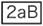
\includegraphics[width=0.35829in,height=0.39306in]{media/image106.png}
\end{quote}
%\end{minipage} & Call Mute \\
\begin{minipage}[t]{\linewidth}\centering
\begin{quote}
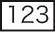
\includegraphics[width=0.275in,height=0.27553in]{media/image107.png}
\end{quote}
%\end{minipage} & Ringer volume is 0 \\
\begin{minipage}[t]{\linewidth}\centering
\begin{quote}
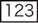
\includegraphics[width=0.21803in,height=0.27708in]{media/image108.png}
\end{quote}
%\end{minipage} & Phone Lock \\
\begin{minipage}[t]{\linewidth}\centering
\begin{quote}

\includegraphics[width=0.24974in,height=0.23611in]{media/image109.png}
\end{quote}
%\end{minipage} & Received Calls \\
\begin{minipage}[t]{\linewidth}\centering
\begin{quote}

\includegraphics[width=0.24974in,height=0.23611in]{media/image110.png}
\end{quote}
%\end{minipage} & Placed Calls \\
\begin{minipage}[t]{\linewidth}\centering
\begin{quote}

\includegraphics[width=0.36249in,height=0.23611in]{media/image111.png}
\end{quote}
%\end{minipage} & Missed Calls \\
\begin{minipage}[t]{\linewidth}\centering
\begin{quote}

\includegraphics[width=0.29306in,height=0.29306in]{media/image112.png}
\end{quote}
%\end{minipage} & Recording box is full \\
\begin{minipage}[t]{\linewidth}\centering
\begin{quote}

\includegraphics[width=0.24619in,height=0.28611in]{media/image113.png}
\end{quote}
%\end{minipage} & A call cannot be recorded \\
\begin{minipage}[t]{\linewidth}\centering
\begin{quote}

\includegraphics[width=0.19653in,height=0.19371in]{media/image114.png}
\end{quote}
%\end{minipage} & Recording starts successfully \\
\begin{minipage}[t]{\linewidth}\centering
\begin{quote}

\includegraphics[width=0.19653in,height=0.19371in]{media/image115.png}
\end{quote}
%\end{minipage} & Recording cannot be started \\
\begin{minipage}[t]{\linewidth}\centering
\begin{quote}

\includegraphics[width=0.25964in,height=0.30625in]{media/image116.png}
\end{quote}
%\end{minipage} & Recording cannot be stopped \\
%\end{longtable}


\includegraphics[width=1.76806in,height=0.28in]{media/image117.png}

Power Indicator LED (Hardware version must be 1.0.0.2 or higher)

%\begin{longtable}[]{@{}
%  >{\raggedright\arraybackslash}p{(\linewidth - 2\tabcolsep) * \real{0.3655}}
%  >{\raggedright\arraybackslash}p{(\linewidth - 2\tabcolsep) * \real{0.6345}}@{}}
%\toprule\noalign{}
\begin{minipage}[b]{\linewidth}\centering
\begin{quote}
LED Status
\end{quote}
%\end{minipage} & \begin{minipage}[b]{\linewidth}\centering
\begin{quote}
Description
\end{quote}
\end{minipage} \\
%\midrule\noalign{}
%\endhead
%\bottomrule\noalign{}
%\endlastfoot
%Solid green & \begin{minipage}[t]{\linewidth}\raggedright
\begin{quote}
The phone is initializing.

The phone is busy.

The phone is idle.

The call is placed on hold or is held.

The phone receives a text message or voice mail.
\end{quote}
\end{minipage} \\
%Fast flashing green (300ms) &
\begin{minipage}[t]{\linewidth}\raggedright
\begin{quote}
The phone is ringing.

The call is muted.
\end{quote}
\end{minipage} \\
%Off & \begin{minipage}[t]{\linewidth}\raggedright
\begin{quote}
The phone is powered off.
\end{quote}
\end{minipage} \\
%\end{longtable}

\begin{quote}
Line key LED
\end{quote}

%\begin{longtable}[]{@{}
%  >{\raggedright\arraybackslash}p{(\linewidth - 2\tabcolsep) * \real{0.3655}}
%  >{\raggedright\arraybackslash}p{(\linewidth - 2\tabcolsep) * \real{0.6345}}@{}}
%\toprule\noalign{}
\begin{minipage}[b]{\linewidth}\centering
\begin{quote}
LED Status
\end{quote}
%\end{minipage} & \begin{minipage}[b]{\linewidth}\centering
\begin{quote}
Description
\end{quote}
\end{minipage} \\
%\midrule\noalign{}
%\endhead
%\bottomrule\noalign{}
%\endlastfoot
%Solid green & \begin{minipage}[t]{\linewidth}\raggedright
\begin{quote}
The line is in conversation.

The line is seized.
\end{quote}
\end{minipage} \\
%Fast flashing green & \begin{minipage}[t]{\linewidth}\raggedright
\begin{quote}
The line receives an incoming call.
\end{quote}
\end{minipage} \\
%Slow flashing green & \begin{minipage}[t]{\linewidth}\raggedright
\begin{quote}
The call is placed on hold.
\end{quote}
\end{minipage} \\
%Off & \begin{minipage}[t]{\linewidth}\raggedright
\begin{quote}
The line is inactive.
\end{quote}
\end{minipage} \\
%\end{longtable}

\begin{quote}
Line key LED (configured as a BLF key or a BLF List key)
\end{quote}

%\begin{longtable}[]{@{}
%  >{\raggedright\arraybackslash}p{(\linewidth - 2\tabcolsep) * \real{0.3655}}
%  >{\raggedright\arraybackslash}p{(\linewidth - 2\tabcolsep) * \real{0.6345}}@{}}
%\toprule\noalign{}
\begin{minipage}[b]{\linewidth}\centering
LED Status
%\end{minipage} & \begin{minipage}[b]{\linewidth}\centering
Description
\end{minipage} \\
%\midrule\noalign{}
%\endhead
%\bottomrule\noalign{}
%\endlastfoot
%Solid green & \begin{minipage}[t]{\linewidth}\raggedright
\begin{quote}
The monitored user is idle.
\end{quote}
\end{minipage} \\
%Fast flashing green (200ms) &
\begin{minipage}[t]{\linewidth}\raggedright
\begin{quote}
The monitored user receives an incoming call.
\end{quote}
\end{minipage} \\
%Slow flashing green (500ms) &
\begin{minipage}[t]{\linewidth}\raggedright
\begin{quote}
The monitored user is dialing.

The monitored user is talking.

The monitored user's conversation is placed on hold (This status
requires server support).
\end{quote}
\end{minipage} \\
%Slow flashing green (1s) & \begin{minipage}[t]{\linewidth}\raggedright
\begin{quote}
The call is parked against the monitored user's phone number.
\end{quote}
\end{minipage} \\
%Off & \begin{minipage}[t]{\linewidth}\raggedright
\begin{quote}
The monitored user does not exist.
\end{quote}
\end{minipage} \\
%\end{longtable}

\begin{quote}
Memory key LED (configured as a BLF key or a BLF List key)
\end{quote}

%\begin{longtable}[]{@{}
%  >{\raggedright\arraybackslash}p{(\linewidth - 2\tabcolsep) * \real{0.3655}}
%  >{\raggedright\arraybackslash}p{(\linewidth - 2\tabcolsep) * \real{0.6345}}@{}}
%\toprule\noalign{}
\begin{minipage}[b]{\linewidth}\centering
\begin{quote}
LED Status
\end{quote}
%\end{minipage} & \begin{minipage}[b]{\linewidth}\centering
\begin{quote}
Description
\end{quote}
\end{minipage} \\
%\midrule\noalign{}
%\endhead
%\bottomrule\noalign{}
%\endlastfoot
%Solid green & \begin{minipage}[t]{\linewidth}\raggedright
\begin{quote}
The monitored user is idle.
\end{quote}
\end{minipage} \\
%Fast flashing red (200ms) & \begin{minipage}[t]{\linewidth}\raggedright
\begin{quote}
The monitored user receives an incoming call.
\end{quote}
\end{minipage} \\
%Solid red & \begin{minipage}[t]{\linewidth}\raggedright
\begin{quote}
The monitored user is dialing.

The monitored user is talking.
\end{quote}
\end{minipage} \\
%Slow flashing red (1s) & \begin{minipage}[t]{\linewidth}\raggedright
\begin{quote}
The call is parked against the monitored user's phone number.

The monitored user's conversation is placed on hold (This status
requires server support).
\end{quote}
\end{minipage} \\
%Off & \begin{minipage}[t]{\linewidth}\raggedright
\begin{quote}
The monitored user does not exist.
\end{quote}
\end{minipage} \\
%\end{longtable}

%\begin{longtable}[]{@{}
%  >{\raggedright\arraybackslash}p{(\linewidth - 0\tabcolsep) * \real{1.0000}}@{}}
%\toprule\noalign{}
\begin{minipage}[b]{\linewidth}\raggedright
The above introduces the default LED status. The statuses of the power
indicator LED and BLF key are configurable via web user interface. For
more information, refer to
Yealink\_SIP-T2xP\_IP\_Phones\_Administrator\_Guide.
\end{minipage} \\
%\midrule\noalign{}
%\endhead
%\bottomrule\noalign{}
%\endlastfoot
%\end{longtable}

Note

\begin{quote}
Two ways to customize configurations of your SIP-T28P IP phone:
\end{quote}

\begin{itemize}
\item
The user interface on the IP phone.
\item
The user interface in a web browser on your PC.
\end{itemize}

\begin{quote}
The hardware components keypad and LCD screen constitute the phone user
interface, which allows the user to execute all call operation tasks and
basic configuration changes directly on the phone. In addition, you can
use the web user interface to access all configuration settings. In many
cases, either the phone user interface and/or the web user interface
interchangeably. However, in some cases, it is only possible to use one
or the other interface to operate the phone and change settings.
\end{quote}


\includegraphics[width=1.96417in,height=0.24333in]{media/image122.png}

\begin{quote}
You can customize your phone by pressing the Menu soft key to access the
phone user interface. The Advanced Settings option is only accessible to
the administrator, and the default administrator password is ``admin''
(case-sensitive). For more information on customizing your phone with
the available options from the phone user interface, refer to
Customizing Your Phone on page 19.
\end{quote}


\includegraphics[width=1.79514in,height=0.24333in]{media/image123.png}

\begin{quote}
In addition to the phone user interface, you can also customize your
phone via web user interface. In order to access the web user interface,
you need to know the IP address of your new phone. To obtain the IP
address, press the OK key on the phone when the phone is idle. Enter the
IP address (e.g., http://192.168.0.10 or 192.168.0.10) in the address
bar of a web browser on your PC. The default administrator user name and
password are both ``admin'' (case-sensitive).

The options you can use to customize the IP phone via phone user
interface and/or via web user interface are listed in the following
table:
\end{quote}

%\begin{longtable}[]{@{}
%  >{\raggedright\arraybackslash}p{(\linewidth - 4\tabcolsep) * \real{0.4390}}
%  >{\centering\arraybackslash}p{(\linewidth - 4\tabcolsep) * \real{0.2868}}
%  >{\centering\arraybackslash}p{(\linewidth - 4\tabcolsep) * \real{0.2742}}@{}}
%\toprule\noalign{}
\begin{minipage}[b]{\linewidth}\centering
\begin{quote}
Options
\end{quote}
%\end{minipage} & \begin{minipage}[b]{\linewidth}\centering
\begin{quote}
Phone User Interface
\end{quote}
%\end{minipage} & \begin{minipage}[b]{\linewidth}\centering
\begin{quote}
Web User Interface
\end{quote}
\end{minipage} \\
%\midrule\noalign{}
%\endhead
%\bottomrule\noalign{}
%\endlastfoot
% \begin{minipage}[t]{\linewidth}\raggedright
\begin{quote}
Status
\end{quote}
%\end{minipage} &
%\multirow{7}{=}{\begin{minipage}[t]{\linewidth}\centering
\begin{quote}
%√
\end{quote}
%\end{minipage}} & \multirow{7}{=}{√} \\
\begin{minipage}[t]{\linewidth}\raggedright
\begin{quote}
-\/-IP Address
\end{quote}
\end{minipage} \\
\begin{minipage}[t]{\linewidth}\raggedright
\begin{quote}
-\/-MAC
\end{quote}
\end{minipage} \\
\begin{minipage}[t]{\linewidth}\raggedright
\begin{quote}
-\/-Firmware
\end{quote}
\end{minipage} \\
\begin{minipage}[t]{\linewidth}\raggedright
\begin{quote}
-\/-Network
\end{quote}
\end{minipage} \\
\begin{minipage}[t]{\linewidth}\raggedright
\begin{quote}
-\/-Phone
\end{quote}
\end{minipage} \\
\begin{minipage}[t]{\linewidth}\raggedright
\begin{quote}
-\/-Accounts
\end{quote}
\end{minipage} \\
% \begin{minipage}[t]{\linewidth}\raggedright
\begin{quote}
Basic Phone Settings
\end{quote}
%\end{minipage} & & \multirow{7}{=}{√} \\
% \begin{minipage}[t]{\linewidth}\raggedright
\begin{quote}
-\/-Contrast
\end{quote}
%\end{minipage} &
%\multirow{4}{=}{
\includegraphics[width=1.45in,height=0.78333in]{media/image124.png}} \\
\begin{minipage}[t]{\linewidth}\raggedright
\begin{quote}
-\/-Backlight
\end{quote}
\end{minipage} \\
\begin{minipage}[t]{\linewidth}\raggedright
\begin{quote}
-\/-Language
\end{quote}
\end{minipage} \\
\begin{minipage}[t]{\linewidth}\raggedright
\begin{quote}
-\/-Time \& Date
\end{quote}
\end{minipage} \\
\begin{minipage}[t]{\linewidth}\raggedright
\begin{quote}
-\/-Administrator Password
\end{quote}
%\end{minipage} & \begin{minipage}[t]{\linewidth}\centering
\begin{quote}
%√
\end{quote}
\end{minipage} \\
\begin{minipage}[t]{\linewidth}\raggedright
\begin{quote}
-\/-Key as Send
\end{quote}
%\end{minipage} & \begin{minipage}[t]{\linewidth}\centering
\begin{quote}
%√
\end{quote}
\end{minipage} \\
%\end{longtable}

%\begin{longtable}[]{@{}
%  >{\raggedright\arraybackslash}p{(\linewidth - 4\tabcolsep) * \real{0.4390}}
%  >{\raggedright\arraybackslash}p{(\linewidth - 4\tabcolsep) * \real{0.2868}}
%  >{\raggedright\arraybackslash}p{(\linewidth - 4\tabcolsep) * \real{0.2742}}@{}}
%\toprule\noalign{}
\begin{minipage}[b]{\linewidth}\centering
\begin{quote}
Options
\end{quote}
%\end{minipage} & \begin{minipage}[b]{\linewidth}\raggedright
\begin{quote}
Phone User Interface
\end{quote}
%\end{minipage} & \begin{minipage}[b]{\linewidth}\raggedright
\begin{quote}
Web User Interface
\end{quote}
\end{minipage} \\
%\midrule\noalign{}
%\endhead
%\bottomrule\noalign{}
%\endlastfoot
% \begin{minipage}[t]{\linewidth}\raggedright
\begin{quote}
-\/- Phone Lock
\end{quote}
%\end{minipage} &
%\multirow{2}{=}{
\includegraphics[width=1.45in,height=0.33333in]{media/image125.png}}
%& \multirow{15}{=}{} \\
\begin{minipage}[t]{\linewidth}\raggedright
\begin{quote}
-\/-Ring Tones
\end{quote}
\end{minipage} \\
% \begin{minipage}[t]{\linewidth}\raggedright
\begin{quote}
-\/-Contact Management
\end{quote}
%\end{minipage} & × \\
% \begin{minipage}[t]{\linewidth}\raggedright
\begin{quote}
-\/-Directory
\end{quote}
%\end{minipage} & × \\
% \begin{minipage}[t]{\linewidth}\raggedright
\begin{quote}
-\/-Local Directory
\end{quote}
%\end{minipage} &
%\multirow{2}{=}{
\includegraphics[width=1.45in,height=0.33667in]{media/image126.png}} \\
\begin{minipage}[t]{\linewidth}\raggedright
\begin{quote}
-\/-Blacklist
\end{quote}
\end{minipage} \\
% \begin{minipage}[t]{\linewidth}\raggedright
\begin{quote}
-\/-Remote Phone Book
\end{quote}
%\end{minipage} & × \\
\begin{minipage}[t]{\linewidth}\raggedright
\begin{quote}
-\/-Call History Management
\end{quote}
%\end{minipage} & \begin{minipage}[t]{\linewidth}\centering
\begin{quote}
%√
\end{quote}
\end{minipage} \\
% \begin{minipage}[t]{\linewidth}\raggedright
\begin{quote}
-\/-Logo Customization
\end{quote}
%\end{minipage} & × \\
\begin{minipage}[t]{\linewidth}\raggedright
\begin{quote}
-\/-DSS Keys
\end{quote}
%\end{minipage} & \begin{minipage}[t]{\linewidth}\centering
\begin{quote}
%√
\end{quote}
\end{minipage} \\
\begin{minipage}[t]{\linewidth}\raggedright
\begin{quote}
-\/-Account Registration
\end{quote}
%\end{minipage} & \begin{minipage}[t]{\linewidth}\centering
\begin{quote}
%√
\end{quote}
\end{minipage} \\
% \begin{minipage}[t]{\linewidth}\raggedright
\begin{quote}
-\/-Dial Plan
\end{quote}
%\end{minipage} & × \\
% \begin{minipage}[t]{\linewidth}\raggedright
\begin{quote}
-\/-Emergency Number
\end{quote}
%\end{minipage} & × \\
% \begin{minipage}[t]{\linewidth}\raggedright
\begin{quote}
-\/-Live Dialpad
\end{quote}
%\end{minipage} & × \\
\begin{minipage}[t]{\linewidth}\raggedright
\begin{quote}
-\/-Hotline
\end{quote}
%\end{minipage} & \begin{minipage}[t]{\linewidth}\centering
\begin{quote}
%√
\end{quote}
\end{minipage} \\
% \begin{minipage}[t]{\linewidth}\raggedright
\begin{quote}
Basic Call Features
\end{quote}
%\end{minipage} & & \multirow{15}{=}{√} \\
% \begin{minipage}[t]{\linewidth}\raggedright
\begin{quote}
-\/-Recent Call In Dialing
\end{quote}
%\end{minipage} & × \\
% \begin{minipage}[t]{\linewidth}\raggedright
\begin{quote}
-\/-Auto Answer
\end{quote}
%\end{minipage} &
%\multirow{8}{=}{
\includegraphics[width=1.45in,height=1.68in]{media/image127.png}} \\
\begin{minipage}[t]{\linewidth}\raggedright
\begin{quote}
-\/-Auto Redial
\end{quote}
\end{minipage} \\
\begin{minipage}[t]{\linewidth}\raggedright
\begin{quote}
-\/-Call Completion
\end{quote}
\end{minipage} \\
\begin{minipage}[t]{\linewidth}\raggedright
\begin{quote}
-\/-Recall
\end{quote}
\end{minipage} \\
\begin{minipage}[t]{\linewidth}\raggedright
\begin{quote}
-\/-Do Not Disturb (DND)
\end{quote}
\end{minipage} \\
\begin{minipage}[t]{\linewidth}\raggedright
\begin{quote}
-\/-Call Forward
\end{quote}
\end{minipage} \\
\begin{minipage}[t]{\linewidth}\raggedright
\begin{quote}
-\/-Call Transfer
\end{quote}
\end{minipage} \\
\begin{minipage}[t]{\linewidth}\raggedright
\begin{quote}
-\/-Call Waiting
\end{quote}
\end{minipage} \\
% \begin{minipage}[t]{\linewidth}\raggedright
\begin{quote}
-\/-Conference
\end{quote}
%\end{minipage} & × \\
\begin{minipage}[t]{\linewidth}\raggedright
\begin{quote}
-\/-Call Park
\end{quote}
%\end{minipage} & \begin{minipage}[t]{\linewidth}\centering
\begin{quote}
%√
\end{quote}
\end{minipage} \\
\begin{minipage}[t]{\linewidth}\raggedright
\begin{quote}
-\/-Call Pickup
\end{quote}
%\end{minipage} & \begin{minipage}[t]{\linewidth}\centering
\begin{quote}
%√
\end{quote}
\end{minipage} \\
% \begin{minipage}[t]{\linewidth}\raggedright
\begin{quote}
-\/-Anonymous Call
\end{quote}
%\end{minipage} &
%\multirow{2}{=}{
\includegraphics[width=1.45in,height=0.34667in]{media/image128.png}} \\
\begin{minipage}[t]{\linewidth}\raggedright
\begin{quote}
-\/-Anonymous Call Rejection
\end{quote}
\end{minipage} \\
% \begin{minipage}[t]{\linewidth}\raggedright
\begin{quote}
Advanced Phone Features
\end{quote}
%\end{minipage} & & \multirow{9}{=}{√} \\
\begin{minipage}[t]{\linewidth}\raggedright
\begin{quote}
-\/-Busy Lamp Field (BLF)
\end{quote}
%\end{minipage} & \begin{minipage}[t]{\linewidth}\centering
\begin{quote}
%√
\end{quote}
\end{minipage} \\
% \begin{minipage}[t]{\linewidth}\raggedright
\begin{quote}
-\/-BLF List
\end{quote}
%\end{minipage} & × \\
\begin{minipage}[t]{\linewidth}\raggedright
\begin{quote}
-\/-Call Recording
\end{quote}
%\end{minipage} & \begin{minipage}[t]{\linewidth}\centering
\begin{quote}
%√
\end{quote}
\end{minipage} \\
\begin{minipage}[t]{\linewidth}\raggedright
\begin{quote}
-\/-Hot Desking
\end{quote}
%\end{minipage} & \begin{minipage}[t]{\linewidth}\centering
\begin{quote}
%√
\end{quote}
\end{minipage} \\
\begin{minipage}[t]{\linewidth}\raggedright
\begin{quote}
-\/-Intercom
\end{quote}
%\end{minipage} & \begin{minipage}[t]{\linewidth}\centering
\begin{quote}
%√
\end{quote}
\end{minipage} \\
% \begin{minipage}[t]{\linewidth}\raggedright
\begin{quote}
-\/-Multicast Paging
\end{quote}
%\end{minipage} & × \\
% \begin{minipage}[t]{\linewidth}\raggedright
\begin{quote}
-\/-Music on Hold
\end{quote}
%\end{minipage} & × \\
\begin{minipage}[t]{\linewidth}\raggedright
\begin{quote}
-\/-Messages
\end{quote}
%\end{minipage} & \begin{minipage}[t]{\linewidth}\centering
\begin{quote}
%√
\end{quote}
\end{minipage} \\
% \begin{minipage}[t]{\linewidth}\raggedright
\begin{quote}
SIP Account
\end{quote}
%\end{minipage} & & \multirow{2}{=}{√} \\
%\begin{minipage}[t]{\linewidth}\raggedright
\begin{quote}
-\/-User Options
\end{quote}
%\end{minipage} & × \\
\begin{minipage}[t]{\linewidth}\centering
\begin{quote}
Options
\end{quote}
%\end{minipage} & \begin{minipage}[t]{\linewidth}\raggedright
\begin{quote}
Phone User Interface
\end{quote}
%\end{minipage} & \begin{minipage}[t]{\linewidth}\raggedright
\begin{quote}
Web User Interface
\end{quote}
\end{minipage} \\
%\begin{minipage}[t]{\linewidth}\raggedright
\begin{quote}
-\/-Account Status
\end{quote}
%\end{minipage} &
%\multirow{7}{=}{
\includegraphics[width=1.45in,height=1.45333in]{media/image129.png}}
%& \multirow{14}{=}{} \\
\begin{minipage}[t]{\linewidth}\raggedright
\begin{quote}
-\/-Label
\end{quote}
\end{minipage} \\
\begin{minipage}[t]{\linewidth}\raggedright
\begin{quote}
-\/-Display Name
\end{quote}
\end{minipage} \\
\begin{minipage}[t]{\linewidth}\raggedright
\begin{quote}
-\/-Register Name
\end{quote}
\end{minipage} \\
\begin{minipage}[t]{\linewidth}\raggedright
\begin{quote}
-\/-User Name
\end{quote}
\end{minipage} \\
\begin{minipage}[t]{\linewidth}\raggedright
\begin{quote}
-\/-Password
\end{quote}
\end{minipage} \\
\begin{minipage}[t]{\linewidth}\raggedright
\begin{quote}
-\/-SIP Server1/2
\end{quote}
\end{minipage} \\
%\begin{minipage}[t]{\linewidth}\raggedright
\begin{quote}
-\/-Server Option
\end{quote}
%\end{minipage} & × \\
%\begin{minipage}[t]{\linewidth}\raggedright
\begin{quote}
-\/-Registrar Port
\end{quote}
%\end{minipage} & × \\
\begin{minipage}[t]{\linewidth}\raggedright
\begin{quote}
-\/-Outbound Status
\end{quote}
%\end{minipage} & \begin{minipage}[t]{\linewidth}\centering
\begin{quote}
%√
\end{quote}
\end{minipage} \\
\begin{minipage}[t]{\linewidth}\raggedright
\begin{quote}
-\/-Outbound Proxy
\end{quote}
%\end{minipage} & \begin{minipage}[t]{\linewidth}\centering
\begin{quote}
%√
\end{quote}
\end{minipage} \\
%\begin{minipage}[t]{\linewidth}\raggedright
\begin{quote}
-\/-NAT Traversal
\end{quote}
%\end{minipage} & \\
%\begin{minipage}[t]{\linewidth}\raggedright
\begin{quote}
-\/-STUN Status
\end{quote}
%\end{minipage} &
%\multirow{2}{=}{
\includegraphics[width=1.45in,height=0.33333in]{media/image130.png}} \\
\begin{minipage}[t]{\linewidth}\raggedright
\begin{quote}
-\/-STUN Server
\end{quote}
\end{minipage} \\
%\end{longtable}

%\begin{longtable}[]{@{}
%  >{\raggedright\arraybackslash}p{(\linewidth - 0\tabcolsep) * \real{1.0000}}@{}}
%\toprule\noalign{}
\begin{minipage}[b]{\linewidth}\raggedright
The table above lists most of the feature options. Please refer to the
relevant sections for more information.
\end{minipage} \\
%\midrule\noalign{}
%\endhead
%\bottomrule\noalign{}
%\endlastfoot
%\end{longtable}

Note

The following table shows documentations available for the SIP-T28P IP
phone.

%\begin{longtable}[]{@{}
%  >{\raggedright\arraybackslash}p{(\linewidth - 6\tabcolsep) * \real{0.2553}}
%  >{\raggedright\arraybackslash}p{(\linewidth - 6\tabcolsep) * \real{0.2741}}
%  >{\raggedright\arraybackslash}p{(\linewidth - 6\tabcolsep) * \real{0.2151}}
%  >{\centering\arraybackslash}p{(\linewidth - 6\tabcolsep) * \real{0.2555}}@{}}
%\toprule\noalign{}
\begin{minipage}[b]{\linewidth}\centering
Name
%\end{minipage} & \begin{minipage}[b]{\linewidth}\centering
Contents
%\end{minipage} & \begin{minipage}[b]{\linewidth}\centering
Where found
%\end{minipage} & \begin{minipage}[b]{\linewidth}\centering
Language
\end{minipage} \\
%\midrule\noalign{}
%\endhead
%\bottomrule\noalign{}
%\endlastfoot
%\begin{minipage}[t]{\linewidth}\raggedright
\begin{quote}
Quick Start Guide
\end{quote}
%\end{minipage} & Basic call features and phone customizations & In the
%package & English \\
\begin{minipage}[t]{\linewidth}\raggedright
\begin{quote}
User Guide
\end{quote}
%\end{minipage} & Phone/ Web user interface settings Basic call features
%and advanced phone features & On the website & English \\
%\end{longtable}

%\begin{longtable}[]{@{}
%  >{\raggedright\arraybackslash}p{(\linewidth - 0\tabcolsep) * \real{1.0000}}@{}}
%\toprule\noalign{}
\begin{minipage}[b]{\linewidth}\raggedright
You can also download the latest documentations online:

%\href{http://www.yealink.com/SupportDownloadfiles_detail.aspx?CateId=184&flag=142}{http://www.yealink.com/SupportDownloadfiles\_detail.aspx?CateId=184\&flag=142.}
%\end{minipage} \\
%\midrule\noalign{}
%\endhead
%\bottomrule\noalign{}
%\endlastfoot
%\end{longtable}

Note

\begin{quote}
This chapter provides basic installation instructions and information
for obtaining the best performance with the SIP-T28P IP phone. Topics
include:
\end{quote}

\begin{itemize}
\item
Packaging Contents
\item
Phone Installation
\item
Phone Initialization
\item
Phone Status
\item
Basic Network Settings
\item
Registration
\item
Idle Screen
\end{itemize}

\begin{quote}
If you require additional information or assistance with your new phone,
contact your system administrator.

The following components are included in your SIP-T28P IP phone package:
%● SIP-T28P IP phone
\end{quote}


\includegraphics[width=3.9625in,height=2.66361in]{media/image141.png}

\begin{itemize}
\item
Phone Stand
\end{itemize}

\begin{quote}

\includegraphics[width=1.33854in,height=0.64167in]{media/image142.png}
\end{quote}

\begin{itemize}
\item
Handset \& Handset Cord
\end{itemize}

\begin{quote}

\includegraphics[width=0.40903in,height=1.59472in]{media/image143.png}

\includegraphics[width=1.48125in,height=0.83958in]{media/image144.png}
\end{quote}

\begin{itemize}
\item
Ethernet Cable
\end{itemize}

\begin{quote}

\includegraphics[width=1.40694in,height=1.01712in]{media/image145.png}
\end{quote}

\begin{itemize}
\item
Quick Start Guide
\end{itemize}

\begin{quote}

\includegraphics[width=1.21218in,height=0.73264in]{media/image146.png}

Check the list before installation. If you find anything missing,
contact your system administrator.

The following items are optional accessories for your SIP-T28P IP phone.
You need to purchase them separately if required.
\end{quote}

\begin{itemize}
\item
Power Adapter
\end{itemize}

\begin{quote}

\includegraphics[width=1.32083in,height=1.37708in]{media/image151.png}
\end{quote}

\begin{itemize}
\item
Headset
\end{itemize}

\begin{quote}

\includegraphics[width=1.55833in,height=1.32431in]{media/image152.png}

If your phone is already installed, proceed to Phone Initialization on
page 13.

This section introduces how to install the phone:
\end{quote}

\begin{enumerate}
\def\labelenumi{\arabic{enumi})}
\item
Attach the stand
\item
Connect the handset and optional headset
\item
Connect the network and power
\end{enumerate}

\begin{enumerate}
\def\labelenumi{\arabic{enumi})}
\item
Attach the stand
\end{enumerate}


\includegraphics[width=4.33056in,height=1.21736in]{media/image157.png}

\begin{enumerate}
\def\labelenumi{\arabic{enumi})}
\setcounter{enumi}{1}
\item
Connect the handset and optional headset
\end{enumerate}


\includegraphics[width=4.59861in,height=2.26597in]{media/image158.png}

%\begin{longtable}[]{@{}
%>{\raggedright\arraybackslash}p{(\linewidth - 0\tabcolsep) * \real{1.0000}}@{}}
%\toprule\noalign{}
\begin{minipage}[b]{\linewidth}\raggedright
A headset is not included in the packaging contents. Contact your system
administrator for more information.
\end{minipage} \\
%\midrule\noalign{}
%\endhead
%\bottomrule\noalign{}
%\endlastfoot
%\end{longtable}

Note

\begin{enumerate}
\def\labelenumi{\arabic{enumi})}
\setcounter{enumi}{2}
\item
Connect the network and power
\end{enumerate}

\begin{quote}
You have two options for power and network connections. Your system
administrator will advise you which one to use.

%● AC power (Optional) ● Power over Ethernet (PoE)
\end{quote}

%\section{\texorpdfstring{AC Power (Optional)
%}{AC Power (Optional) }}\label{ac-power-optional}

\begin{quote}
To connect the AC power:
\end{quote}

\begin{enumerate}
\def\labelenumi{\arabic{enumi}.}
\item
Connect the DC plug on the power adapter to the DC5V port on the phone
and connect the other end of the power adapter into an electrical
power outlet.
\item
Connect the included or a standard Ethernet cable between the Internet
port on the phone and the one on the wall or switch/hub device port.
\end{enumerate}


\includegraphics[width=5.08458in,height=2.0125in]{media/image159.png}

%\subsection{\texorpdfstring{Power over Ethernet
%}{Power over Ethernet }}\label{power-over-ethernet}

\begin{quote}
With the included or a regular Ethernet cable, the SIP-T28P IP phone can
be powered from a PoE-compliant switch or hub.

To connect the PoE:

1. Connect the Ethernet cable between the Internet port on the phone and
an available port on the in-line power switch/hub.
\end{quote}


\includegraphics[width=5.14583in,height=2.09306in]{media/image160.png}

%\begin{longtable}[]{@{}
%>{\raggedright\arraybackslash}p{(\linewidth - 0\tabcolsep) * \real{1.0000}}@{}}
%\toprule\noalign{}
\begin{minipage}[b]{\linewidth}\raggedright
If in-line power is provided, you don't need to connect the phone to the
power adapter. Make sure the switch/hub is PoE-compliant.

The phone can also share the network with another network device such as
a PC (personal computer). This is an optional connection.

Important! Do not remove power to the phone while it is updating
firmware and configurations.
\end{minipage} \\
%\midrule\noalign{}
%\endhead
%\bottomrule\noalign{}
%\endlastfoot
%\end{longtable}

Note


\includegraphics[width=2.10764in,height=0.28in]{media/image161.png}

\begin{quote}
After your phone is powered on, the system boots up and performs the
following steps: Automatic Phone Initialization

The phone finishes the initialization by loading the saved
configuration. The LCD screen displays ``Initializing, Please Wait''
during this process.

DHCP (Dynamic Host Configuration Protocol)

The phone attempts to contact a DHCP server in your network to obtain
valid network settings (e.g., IP address, subnet mask, default gateway
address and DNS address) by default.
\end{quote}

%\begin{longtable}[]{@{}
%>{\raggedright\arraybackslash}p{(\linewidth - 0\tabcolsep) * \real{1.0000}}@{}}
%\toprule\noalign{}
\begin{minipage}[b]{\linewidth}\raggedright
If your network does not use DHCP, proceed to Basic Network Settings on
page 15.
\end{minipage} \\
%\midrule\noalign{}
%\endhead
%\bottomrule\noalign{}
%\endlastfoot
%end{longtable}

Note


\includegraphics[width=1.46681in,height=0.28in]{media/image162.png}

\begin{quote}
You can view phone status via phone user interface or web user
interface.

Available information of phone status includes:
\end{quote}

\begin{itemize}
\item
Network status (e.g., IPv4 status, IP mode and MAC address).
\item
Phone status (e.g., device model, hardware version, firmware version,
product ID, MAC address and device certificate status).
\item
Account status (e.g., the register status of SIP accounts).
\end{itemize}

%\begin{longtable}[]{@{}
%>{\raggedright\arraybackslash}p{(\linewidth - 0\tabcolsep) * \real{1.0000}}@{}}
%\toprule\noalign{}
\begin{minipage}[b]{\linewidth}\raggedright
You can view device certificate status via phone user interface only.
\end{minipage} \\
%\midrule\noalign{}
%\endhead
%\bottomrule\noalign{}
%\endlastfoot
%\end{longtable}

Note

\begin{quote}
To view the phone status via phone user interface:
\end{quote}

1.

Press

, or press

Menu

-

\textgreater{}

Status

.

2.

Press

or

to scroll through the list and

view

the specific information.

\begin{quote}
To view the phone status via web user interface:
\end{quote}

\begin{enumerate}
\def\labelenumi{\arabic{enumi}.}
\item
Open a web browser on your computer.
\item
Enter the IP address in the browser's address bar, and then press
Enter.
\item
Enter the user name (admin) and password (admin) in the login page.
\item
Click Confirm to login.
\end{enumerate}

\begin{quote}
The phone status is displayed on the first page of the web user
interface.
\end{quote}


\includegraphics[width=2.45792in,height=0.28in]{media/image171.png}

\begin{quote}
If your phone cannot contact a DHCP server for any reason, you need to
configure network settings manually. The IP phone can support either or
both IPv4 and IPv6 addresses.

To configure the IP address mode via phone user interface:

1. Press Menu-\textgreater Settings-\textgreater Advanced Settings
(default password: admin) -\textgreater Network-\textgreater WAN Port.
\end{quote}

2.

Press

or

to

select

IPv4

,

IP

v

6

or

IPv4

\&

IPv6

from

the

IP Mode

field

.

3. Press the Save soft key to accept the change or the Back soft key to
cancel.

\begin{quote}
To configure a static IPv4 address via phone user interface:
\end{quote}

\begin{enumerate}
\def\labelenumi{\arabic{enumi}.}
\item
Press Menu-\textgreater Settings-\textgreater Advanced Settings
(default password: admin) -\textgreater Network-\textgreater WAN
Port-\textgreater IPv4-\textgreater Static IP Client.
\item
Enter the desired values in the IPv4, Subnet Mask, Default Gateway,
IPv4 Pri.DNS and IPv4 Sec.DNS fields respectively.
\item
Press the Save soft key to accept the change or the Back soft key to
cancel.
\end{enumerate}

\begin{quote}
To configure a static IPv6 address via phone user interface:
\end{quote}

\begin{enumerate}
\def\labelenumi{\arabic{enumi}.}
\item
Press Menu-\textgreater Settings-\textgreater Advanced Settings
(default password: admin) -\textgreater Network-\textgreater WAN
Port-\textgreater IPv6-\textgreater Static IP Client.
\item
Enter the desired values in the IPv6 IP, Prefix, Default Gateway, IPv6
Pri.DNS and IPv6 Sec.DNS fields respectively.
\item
Press the Save soft key to accept the change or the Back soft key to
cancel.
\end{enumerate}

\begin{quote}
If you are using an xDSL modem for IPv4 network connection, you can
connect your phone to the Internet via PPPoE mode. Set the WAN port as a
PPPoE port. The PPPoE port will perform a PPP negotiation to obtain the
IP address. Contact your system administrator for the PPPoE user name
and password.

To configure PPPoE via phone user interface:
\end{quote}

\begin{enumerate}
\def\labelenumi{\arabic{enumi}.}
\item
Press Menu-\textgreater Settings-\textgreater Advanced Settings
(default password: admin) -\textgreater Network-\textgreater WAN
Port-\textgreater IPv4-\textgreater PPPoE IP Client.
\item
Enter the user name and password in the corresponding fields.
\item
Press the Save soft key to accept the change or the Back soft key to
cancel.
\end{enumerate}

%\begin{longtable}[]{@{}
%>{\raggedright\arraybackslash}p{(\linewidth - 0\tabcolsep) * \real{1.0000}}@{}}
%\toprule\noalign{}
\begin{minipage}[b]{\linewidth}\raggedright
Wrong network settings may result in inaccessibility of your phone and
may also have an impact on your network performance. For more
information on these parameters, contact your system administrator.
\end{minipage} \\
%\midrule\noalign{}
%\endhead
%\bottomrule\noalign{}
%\endlastfoot
%\end{longtable}

Note

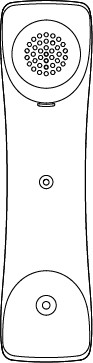
\includegraphics[width=1.36897in,height=0.28in]{media/image180.png}

\begin{quote}
Generally, your phone will be deployed with multiple other phones. In
this case, your system administrator will configure the phone parameters
beforehand, so that after you start up your phone, the phone will be
registered and ready for use. The SIP-T28P IP phone supports up to 6
accounts. If your phone is not registered, you may have to register it.
For more information on how to register your phone, refer to Account
Management on page 62.
\end{quote}


\includegraphics[width=1.22946in,height=0.28in]{media/image181.png}

\begin{quote}
If the phone has successfully started up, the idle screen will be
displayed as below:

The idle screen displays time and date, label of each account, logo and
four soft keys.

You can customize your SIP-T28P IP phone by personally configuring
certain settings, for example, contrast, time \& date and ring tones.
You can add contacts to the phone's local directory manually or from
call history. You can also personalize different ring tones for
different callers.

This chapter provides basic operating instructions for customizing your
phone. Topics include:
\end{quote}

\begin{itemize}
\item
General Settings
\item
Audio Settings
\item
Contact Management
\item
Call History Management
\item
System Customizations
\end{itemize}

\begin{quote}
If you require additional information or assistance with your new phone,
contact your system administrator.
\end{quote}


\includegraphics[width=1.80347in,height=0.28in]{media/image186.png}


\includegraphics[width=0.86288in,height=0.24333in]{media/image187.png}

\begin{quote}
You can configure the contrast of the LCD screen to a comfortable level.

To configure the contrast via phone user interface:
\end{quote}

\begin{enumerate}
\def\labelenumi{\arabic{enumi}.}
\item
Press Menu-\textgreater Settings-\textgreater Basic
Settings-\textgreater Display-\textgreater Contrast.
\item
Press or , or the Switch soft key to increase or decrease the
intensity of contrast.
\end{enumerate}

\begin{quote}
The default contrast level is 6.
\end{quote}

\begin{enumerate}
\def\labelenumi{\arabic{enumi}.}
\setcounter{enumi}{2}
\item
Press the Save soft key to accept the change or the Back soft key to
cancel.
\end{enumerate}

\begin{quote}
Contrast is configurable via web user interface at the path
Settings-\textgreater Preference.
\end{quote}


\includegraphics[width=0.94111in,height=0.24333in]{media/image190.png}

\begin{quote}
You can configure the backlight to adjust the brightness of the LCD
screen. Backlight active level is used to adjust to the backlight
intensity of the LCD screen. Backlight time specifies the delay time to
turn off the backlight when the IP phone is inactive.

You can configure the backlight status on the LCD screen from the
following options:
\end{quote}

\begin{itemize}
\item
Always Off: Backlight is turned off permanently.
\item
Always On: Backlight is on permanently.
\item
15s, 30s, 60s, 120s, 300s, 600s or 1800s: Backlight is turned off when
the phone is inactive after the designated time (in seconds).
\end{itemize}

\begin{quote}
To configure the backlight via phone user interface:
\end{quote}

1. Press Menu-\textgreater Settings-\textgreater Basic
Settings-\textgreater Display-\textgreater Backlight.

2.

Press

or

, or the

Switch

soft key

to

select the desired level from the

Backlight Level

field.

3.

Press

or

, or the

Switch

soft key

to

select the desired type from the

Backlight Time

field.

4. Press the Save soft key to accept the change or the Back soft key to
cancel.

\begin{quote}
Backlight is configurable via web user interface at the path
Settings-\textgreater Preference.
\end{quote}


\includegraphics[width=1.00538in,height=0.24333in]{media/image193.png}

\begin{quote}
The default language of the phone user interface is English. If the
language of your web browser is not supported by the phone, the web user
interface will use English by default. You can change the language for
the phone user interface and the web user interface respectively.

To change the language for the phone user interface:
\end{quote}

1. Press Menu-\textgreater Settings-\textgreater Basic
Settings-\textgreater Language.

2.

Press

or

to select the desired language.

3. Press the Save soft key to accept the change.

\begin{quote}
Text displayed on the LCD screen will change to the selected language.

To change the language for the web user interface:
\end{quote}

\begin{enumerate}
\def\labelenumi{\arabic{enumi}.}
\item
Click on Settings-\textgreater Preference.
\item
Select the desired language from the pull-down list of Language.
\item
Click Confirm to accept the change.
\end{enumerate}

\begin{quote}
Text displayed on the web user interface will change to the selected
language.

The time and date are displayed on the LCD screen when the phone is
idle. If the phone cannot obtain the time and date from the Simple
Network Time Protocol (SNTP) server, you need to configure the time and
date manually. For more information on the SNTP server, contact your
system administrator.

To configure the SNTP settings via phone user interface:
\end{quote}

1. Press Menu-\textgreater Settings-\textgreater Basic
Settings-\textgreater Time \& Date-\textgreater SNTP Settings.

\begin{enumerate}
\def\labelenumi{\arabic{enumi}.}
\setcounter{enumi}{2}
\item
Press or , or the Switch soft key to select the time zone that applies
to your area from the Time Zone field.
\end{enumerate}

\begin{quote}
The default time zone is "+8 China(Beijing)".
\end{quote}

\begin{enumerate}
\def\labelenumi{\arabic{enumi}.}
\setcounter{enumi}{3}
\item
Enter the domain names or IP addresses in the NTP Server 1 and NTP
Server 2 fields respectively.
\end{enumerate}

\begin{quote}
5.
\end{quote}

Press

or

, or the

Switch

soft key

to select

the desired value

from the

Daylight Saving

field.

6. Press the Save soft key to accept the change or the Back soft key to
cancel.

Note Please refer to Appendix A - Time Zones for the list of available
time zones on the IP phone.

\begin{quote}
To configure the time and date manually via phone user interface:
\end{quote}

\begin{enumerate}
\def\labelenumi{\arabic{enumi}.}
\item
Press Menu-\textgreater Settings-\textgreater Basic
Settings-\textgreater Time \& Date-\textgreater Manual Settings.
\item
Enter the specific date in the Date field.
\item
Enter the specific time in the Time field.
\item
Press the Save soft key to accept the change.
\end{enumerate}

\begin{quote}
The date and time displayed on the LCD screen will change accordingly.

To configure the time and date format via phone user interface:
\end{quote}

\begin{enumerate}
\def\labelenumi{\arabic{enumi}.}
\item
Press Menu-\textgreater Settings-\textgreater Basic
Settings-\textgreater Time \& Date-\textgreater Time \& Date Format.
\item
Press or , or the Switch soft key to select the desired time format
from the Time Format field.
\item
Press or , or the Switch soft key to select the desired date format
from the
\end{enumerate}

\begin{quote}
Date Format field.
\end{quote}

\begin{enumerate}
\def\labelenumi{\arabic{enumi}.}
\setcounter{enumi}{3}
\item
Press the Save soft key to accept the change or the Back soft key to
cancel.
\end{enumerate}

\begin{quote}
There are 7 available date formats. For example, for the date format
``WWW DD MMM'', ``WWW'' represents the abbreviation of the weekday,
``DD'' represents the two-digit day, and ``MMM'' represents the first
three letters of the month.

The date formats available:
\end{quote}

%\begin{longtable}[]{@{}
%>{\centering\arraybackslash}p{(\linewidth - 2\tabcolsep) * \real{0.4917}}
%>{\centering\arraybackslash}p{(\linewidth - 2\tabcolsep) * \real{0.5083}}@{}}
%\toprule\noalign{}
\begin{minipage}[b]{\linewidth}\centering
Date Format
%\end{minipage} & \begin{minipage}[b]{\linewidth}\centering
\begin{quote}
Example (2014-7-26)
\end{quote}
\end{minipage} \\
%\midrule\noalign{}
%\endhead
%\bottomrule\noalign{}
%\endlastfoot
%WWW MMM DD & \begin{minipage}[t]{\linewidth}\centering
\begin{quote}
Sat Jul 26
\end{quote}
\end{minipage} \\
%DD-MMM-YY & 26-Jul-14 \\
%YYYY-MM-DD & \begin{minipage}[t]{\linewidth}\centering
\begin{quote}
2014-07-26
\end{quote}
\end{minipage} \\
%\begin{minipage}[t]{\linewidth}\centering
\begin{quote}
DD/MM/YYYY
\end{quote}
%\end{minipage} & 26/07/2014 \\
\begin{minipage}[t]{\linewidth}\centering
\begin{quote}
MM/DD/YY
\end{quote}
%\end{minipage} & 07/26/14 \\
\begin{minipage}[t]{\linewidth}\centering
\begin{quote}
DD MMM YYYY
\end{quote}
%\end{minipage} & \begin{minipage}[t]{\linewidth}\centering
\begin{quote}
26 Jul 2014
\end{quote}
\end{minipage} \\
%WWW DD MMM & \begin{minipage}[t]{\linewidth}\centering
\begin{quote}
Sat 26 Jul
\end{quote}
\end{minipage} \\
%\end{longtable}

\begin{quote}
Time and date is configurable via web user interface at the path
Settings-\textgreater Time \& Date.

The Advanced Settings option is only accessible to the administrator.
The default administrator password is ``admin''. For security reasons,
you should change the default administrator password as soon as
possible.

To change the administrator password via phone user interface:
\end{quote}

\begin{enumerate}
\def\labelenumi{\arabic{enumi}.}
\item
Press Menu-\textgreater Settings-\textgreater Advanced Settings
(default password: admin) -\textgreater Set Password.
\item
Enter the old password in the Current PWD field.
\item
Enter the new password in the New PWD field.
\item
Re-enter the new password in the Confirm PWD field.
\item
Press the Save soft key to accept the change or the Back soft key to
cancel.
\end{enumerate}

\begin{quote}
Administrator password is configurable via web user interface at the
path Security-\textgreater Password.
\end{quote}

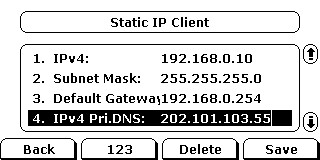
\includegraphics[width=1.15672in,height=0.24333in]{media/image220.png}

\begin{quote}
You can set the "\#" or "*" to perform as a send key while dialing.

To configure key as send via phone user interface:
\end{quote}

1. Press Menu-\textgreater Features-\textgreater Key as Send.

2.

Press

or

, or the

Switch

soft key

to

select

\#

or

*

from

the

Key as

Send

field

,

or

select

Disable

d

to disable this feature

.

3. Press the Save soft key to accept the change or the Back soft key to
cancel.

\begin{quote}
Key as send is configurable via web user interface at the path
Features-\textgreater General Information.

You can lock your phone temporarily when you are not using it. This
feature helps to protect your phone from unauthorized use.

Phone lock consists of the following:

Menu Key: The Menu soft key and MESSAGE key are locked. You cannot

access the menu of the phone until unlocked.

Function Keys: The function keys are locked. You cannot use the MESSAGE,
RD, CONF, HOLD, MUTE, TRAN, OK, X, navigation keys, soft keys, line keys
and memory keys until unlocked.
\end{quote}

All Keys: All keys are locked except the Volume key. You are only
allowed

\begin{quote}
to dial emergency numbers, reject incoming calls by pressing the X key,
answer incoming calls by lifting the handset, pressing the Speakerphone
key, the HEADSET key or the OK key, place an active call on hold by
pressing the Hold soft key or the HOLD key, resume the held call by
pressing the Resume soft key or the HOLD key, and end the call by
pressing the X key, hanging up the handset, pressing the Speakerphone
key.
\end{quote}

%\begin{longtable}[]{@{}
%>{\raggedright\arraybackslash}p{(\linewidth - 0\tabcolsep) * \real{1.0000}}@{}}
%\toprule\noalign{}
\begin{minipage}[b]{\linewidth}\raggedright
The emergency number setting, if desired, must be made before lock
activation. For more information, refer to Emergency Number on page 70.
\end{minipage} \\
%\midrule\noalign{}
%\endhead
%\bottomrule\noalign{}
%\endlastfoot
%\end{longtable}

Note

\begin{quote}
To activate the phone lock via phone user interface:

1. Press Menu-\textgreater Settings-\textgreater Advanced Settings
(default password: admin) -\textgreater Phone Lock.

2.

Lock field.
\end{quote}

Press

or

, or the

Switch

soft key

to

select

the

desired type from

the

Phone

\begin{enumerate}
\def\labelenumi{\arabic{enumi}.}
\setcounter{enumi}{2}
\item
Press the Save soft key to accept the change.
\item

\includegraphics[width=0.29514in,height=0.1999in]{media/image229.png}Long
press to lock the phone immediately when the phone is idle.
\end{enumerate}

T

he LCD screen prompts

``

Phone

locked

.

''

and

displays

the

icon

.

\begin{quote}

\includegraphics[width=0.29499in,height=0.19792in]{media/image229.png}You
can specify the interval (in seconds) to automatically lock the phone
instead of long pressing .

To configure the interval of automatic phone lock via web user
interface:
\end{quote}

\begin{enumerate}
\def\labelenumi{\arabic{enumi}.}
\item
Click on Features-\textgreater Phone Lock.
\item
Enter the desired interval in the Phone Lock Time Out
(0\textasciitilde3600s) field.
\item
Click Confirm to accept the change.
\end{enumerate}

%\begin{longtable}[]{@{}
%>{\raggedright\arraybackslash}p{(\linewidth - 0\tabcolsep) * \real{1.0000}}@{}}
%\toprule\noalign{}
\begin{minipage}[b]{\linewidth}\centering

\includegraphics[width=0.28542in,height=0.2in]{media/image236.png}The
default interval is 0 second, that is, you need to long press to lock
the phone.

The interval of automatic phone lock is configurable via web user
interface only.
\end{minipage} \\
%\midrule\noalign{}
%\endhead
%\bottomrule\noalign{}
%\endlastfoot
%\end{longtable}

Note

\begin{quote}
To unlock the phone, you must know the phone unlock PIN of the phone.
The default phone unlock PIN is ``123''.

To change the phone unlock PIN via phone user interface:
\end{quote}

\begin{enumerate}
\def\labelenumi{\arabic{enumi}.}
\item
Press Menu-\textgreater Settings-\textgreater Basic
Settings-\textgreater Change PIN.
\item
Enter the old PIN in the Current PIN field.
\item
Enter the new PIN in the New PIN field.
\item
Re-enter the new password in the Confirm PIN field.
\item
Press the Save soft key to accept the change or the Back soft key to
cancel.
\end{enumerate}

Note The unlock PIN length must be within 15 digits.

\begin{quote}
To unlock the phone via phone user interface:
\end{quote}

\begin{enumerate}
\def\labelenumi{\arabic{enumi}.}
\item
Press any locked key, the LCD screen prompts ``Please Enter PIN''.
\item
Enter the PIN in the Phone Unlock PIN field.
\item
Press the OK soft key to unlock the phone.
\end{enumerate}

\begin{quote}
The
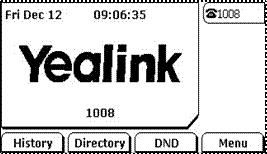
\includegraphics[width=0.12639in,height=0.14712in]{media/image231.png}
icon disappears from the LCD screen.

You can long press

\includegraphics[width=0.29218in,height=0.19375in]{media/image229.png}
or wait for a period of time (if configured) to lock the phone again.
\end{quote}

Note You can also unlock the phone by administrator password. When you
enter the administrator password to unlock the phone, the phone will
turn to the Reset Phone PIN screen.

\begin{quote}
To deactivate the phone lock via phone user interface:

1. Press Menu-\textgreater Settings-\textgreater Advanced Settings
(default password: admin) -\textgreater Phone Lock.

2.

field.
\end{quote}

Press

or

, or the

Switch

soft key

to select

Disable

d

from

the

Phone

Lock

3. Press the Save soft key to accept the change.

\begin{quote}
Phone lock is configurable via web user interface at the path
Features-\textgreater Phone Lock.
\end{quote}

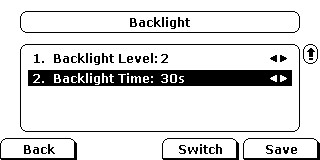
\includegraphics[width=1.615in,height=0.28in]{media/image243.png}

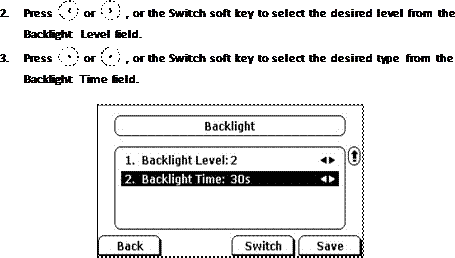
\includegraphics[width=0.80928in,height=0.24333in]{media/image244.png}

\begin{quote}
You can press the Volume key to adjust the ringer volume when the phone
is idle. You can also press the Volume key to adjust the receiver volume
of currently engaged audio devices (handset, speakerphone or headset)
when the phone is in use.

To adjust the volume when the phone is idle:
\end{quote}

1.

Press

to adjust the ringer volume

.

%\begin{longtable}[]{@{}
%>{\raggedright\arraybackslash}p{(\linewidth - 0\tabcolsep) * \real{1.0000}}@{}}
%\toprule\noalign{}
\begin{minipage}[b]{\linewidth}\raggedright
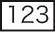
\includegraphics[width=0.12778in,height=0.12778in]{media/image107.png}If
the ringer volume is adjusted to minimum, the icon will appear on the
LCD screen.
\end{minipage} \\
%\midrule\noalign{}
%\endhead
%\bottomrule\noalign{}
%\endlastfoot
%\end{longtable}

Note

\begin{quote}
To adjust the volume when the phone is during a call:

1. Press

\includegraphics[width=0.78125in,height=0.14583in]{media/image246.png}
to adjust the volume of currently engaged audio device (handset,
speakerphone or headset).
\end{quote}


\includegraphics[width=1.08569in,height=0.24333in]{media/image251.png}

\begin{quote}
Ring tones are used to indicate incoming calls. You can select different
ring tones to distinguish different accounts registered on your phone,
or to distinguish your phone from your neighbor's.

To select a ring tone for the phone via phone user interface:
\end{quote}

1. Press Menu-\textgreater Settings-\textgreater Basic Settings
-\textgreater Sound-\textgreater Ring Tones-\textgreater Common.

2.

Press

or

to select the desired ring tone.

3. Press the Save soft key to accept the change or the Back soft key to
cancel.

\begin{quote}
A ring tone for the phone is configurable via web user interface at the
path Settings-\textgreater Preference-\textgreater Ring Type.

To select a ring tone for the account via phone user interface:
\end{quote}

1. Press Menu-\textgreater Settings-\textgreater Basic Settings
-\textgreater Sound-\textgreater Ring Tones.

2.

Press

or

to select the desired

account

and then press the

Enter

soft k

ey

.

3.

Press or to select the desired ring tone.

If Common is selected, this account will use the ring tone selected for
the phone.

4. Press the Save soft key to accept the change or the Back soft key to
cancel.

\begin{quote}
A ring tone for the account is configurable via web user interface at
the path Account-\textgreater Basic-\textgreater Ring Type.
\end{quote}

%\begin{longtable}[]{@{}
%>{\raggedright\arraybackslash}p{(\linewidth - 0\tabcolsep) * \real{1.0000}}@{}}
%\toprule\noalign{}
\begin{minipage}[b]{\linewidth}\raggedright
The ring tone for an incoming call on the phone may be different. For
example, when the phone receives an incoming call from a contact stored
in the local directory, it will play the ring tone assigned to the
contact in the contact directory (refer to Adding Contacts). If no ring
tone is assigned to the contact, the phone will play the ring tone
assigned to the associated group (refer to Adding Groups). Otherwise,
the phone will play the ring tone assigned to the account. If no ring
tone is assigned to the contact, the associated group or account, the
phone will play the ring tone assigned to the phone.
\end{minipage} \\
%\midrule\noalign{}
%\endhead
%\bottomrule\noalign{}
%\endlastfoot
%\end{longtable}

Note

\begin{quote}
To upload a custom ring tone for your phone via web user interface:
\end{quote}

\begin{enumerate}
\def\labelenumi{\arabic{enumi}.}
\item
Click on Settings-\textgreater Preference.
\item
Click Browse to locate a ring tone file (the file format must be
*.wav) from your local system.
\item
Click Upload to upload the file.
\end{enumerate}

%\begin{longtable}[]{@{}
%>{\raggedright\arraybackslash}p{(\linewidth - 0\tabcolsep) * \real{1.0000}}@{}}
%\toprule\noalign{}
\begin{minipage}[b]{\linewidth}\raggedright
All custom ring tone files must be no greater than 100KB.

Custom ring tones for your phone can be uploaded via web user interface
only.
\end{minipage} \\
%\midrule\noalign{}
%\endhead
%\bottomrule\noalign{}
%\endlastfoot
%\end{longtable}

Note


\includegraphics[width=2.34083in,height=0.28in]{media/image260.png}

\begin{quote}
This section provides the operating instructions for managing contacts.
Topics include:
\end{quote}

\begin{itemize}
\item
Directory
\item
Local Directory
\item
Blacklist
\item
Remote Phone Book
\end{itemize}


\includegraphics[width=0.92629in,height=0.24333in]{media/image261.png}

\begin{quote}
Directory provides easy access to frequently used lists. The lists may
contain Local Directory, History, Remote Phone Book and LDAP.

To configure the directory via web user interface:
\end{quote}

\begin{enumerate}
\def\labelenumi{\arabic{enumi}.}
\item
Click on Directory-\textgreater Setting.
\item
In the Directory block, select the desired list from the Disabled
column and then click
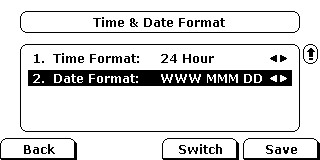
\includegraphics[width=0.21414in,height=0.15972in]{media/image262.png}
.
\end{enumerate}

\begin{quote}
The selected list appears in the Enabled column.
\end{quote}

\begin{enumerate}
\def\labelenumi{\arabic{enumi}.}
\setcounter{enumi}{2}
\item
Repeat step 2 to add more lists to the Enabled column.
\item
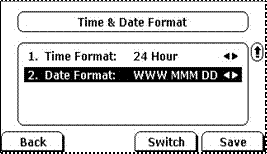
\includegraphics[width=0.21458in,height=0.15064in]{media/image263.png}To
remove a list from the Enabled column, select the desired list and
then click .
\item
To adjust the display order of list, select the desired list and then
click or .
\end{enumerate}

\begin{quote}
The LCD screen will display the list(s) in the adjusted order.
\end{quote}

\begin{enumerate}
\def\labelenumi{\arabic{enumi}.}
\setcounter{enumi}{5}
\item
Click Confirm to accept the change.
\end{enumerate}

%\begin{longtable}[]{@{}
%>{\raggedright\arraybackslash}p{(\linewidth - 0\tabcolsep) * \real{1.0000}}@{}}
%\toprule\noalign{}
\begin{minipage}[b]{\linewidth}\raggedright
Directory is configurable via web user interface only.
\end{minipage} \\
%\midrule\noalign{}
%\endhead
%\bottomrule\noalign{}
%\endlastfoot
%\end{longtable}

Note

\begin{quote}
To view the directory via phone user interface:
\end{quote}

1. Press the Directory soft key when the phone is idle.

\begin{quote}
The LCD screen displays the list(s) in the directory.

If there is only one list in the directory, press the Directory soft key
to enter this list directly.
\end{quote}


\includegraphics[width=1.43361in,height=0.24333in]{media/image272.png}

\begin{quote}
The built-in phone directory can store the names and phone numbers of
your contacts. You can store up to 1000 contacts and 5 groups in your
phone\textquotesingle s local directory. You can add new groups and
contacts, edit, delete or search for a contact, or simply dial a contact
number from the local directory.
\end{quote}

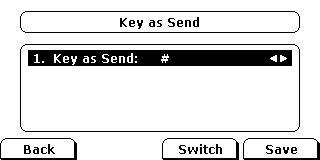
\includegraphics[width=1.24242in,height=0.21in]{media/image273.png}

\begin{quote}
To add a group to the local directory:
\end{quote}

\begin{enumerate}
\def\labelenumi{\arabic{enumi}.}
\item
Press the Directory soft key.
\end{enumerate}

\begin{quote}
The IP phone enters the local directory directly as there is only Local
Directory enabled in the directory by default.

If Local Directory is removed from the directory, press
Menu-\textgreater Directory-\textgreater Local Directory to enter the
local directory.
\end{quote}

\begin{enumerate}
\def\labelenumi{\arabic{enumi}.}
\setcounter{enumi}{1}
\item
Press the Add Group soft key.
\item
Enter the desired group name in the Name field.
\item
Press or , or the Switch soft key to select the desired group ring
tone from the Ring field.
\end{enumerate}

\begin{quote}
If Auto is selected, this group will use the ring tone specified for the
contact. If no ring tone is specified for the contact, it will then play
the ring tone specified for the account. For more information on ring
tone for the account, refer to Ring Tones on page 29.
\end{quote}

\begin{enumerate}
\def\labelenumi{\arabic{enumi}.}
\setcounter{enumi}{4}
\item
Press the Add soft key to accept the change or the Back soft key to
cancel.
\end{enumerate}

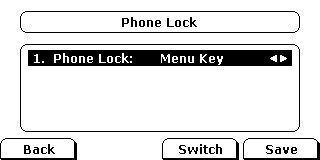
\includegraphics[width=1.22536in,height=0.21in]{media/image278.png}

\begin{quote}
To edit a group in the local directory:
\end{quote}

\begin{enumerate}
\def\labelenumi{\arabic{enumi}.}
\item
Press the Directory soft key.
\end{enumerate}

\begin{quote}
The IP phone enters the local directory directly as there is only Local
Directory enabled in the directory by default.

If Local Directory is removed from the directory, press
Menu-\textgreater Directory-\textgreater Local Directory to enter the
local directory.
\end{quote}

\begin{enumerate}
\def\labelenumi{\arabic{enumi}.}
\setcounter{enumi}{1}
\item
Select the desired group (e.g., Test).
\item
Press the Option soft key, and then select Detail from the prompt
list.
\end{enumerate}

Press

or

to

select

the

group

information and then edit.

\begin{quote}
4.
\end{quote}

5. Press the Save soft key to accept change or the Back soft key to
cancel.


\includegraphics[width=1.33725in,height=0.21in]{media/image283.png}

\begin{quote}
To delete a group from the local directory:
\end{quote}

\begin{enumerate}
\def\labelenumi{\arabic{enumi}.}
\item
Press the Directory soft key.
\end{enumerate}

\begin{quote}
The IP phone enters the local directory directly as there is only Local
Directory enabled in the directory by default.

If Local Directory is removed from the directory, press
Menu-\textgreater Directory-\textgreater Local Directory to enter the
local directory.
\end{quote}

\begin{enumerate}
\def\labelenumi{\arabic{enumi}.}
\setcounter{enumi}{1}
\item
Select the desired group (e.g., Test).
\item
Press the Option soft key, and then select Delete from the prompt
list.
\end{enumerate}

\begin{quote}
The LCD screen prompts ``Delete selected group?''.
\end{quote}

\begin{enumerate}
\def\labelenumi{\arabic{enumi}.}
\setcounter{enumi}{3}
\item
Press the OK soft key to confirm the deletion or the Cancel soft key
to cancel.
\end{enumerate}

\begin{quote}
You can also delete all groups by pressing the Option soft key and then
select Delete All.

For more information, refer to the above steps.
\end{quote}

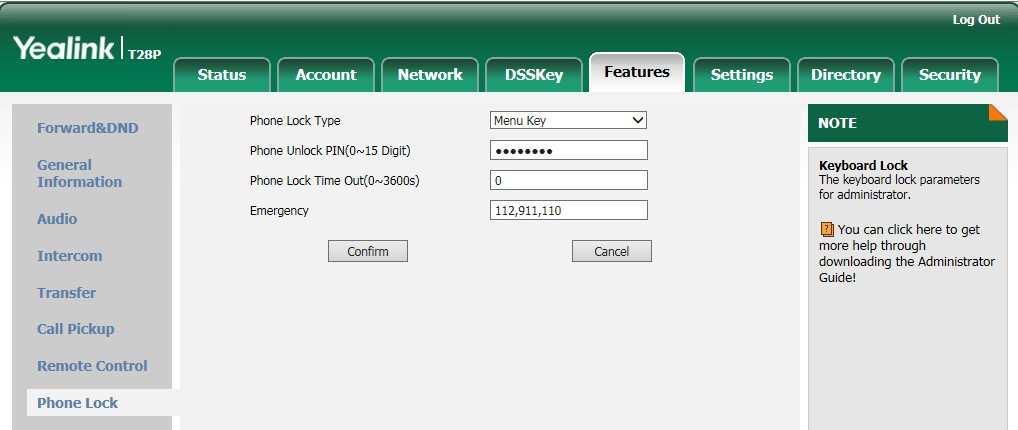
\includegraphics[width=1.35503in,height=0.21in]{media/image286.png}

\begin{quote}
You can add contacts to your local directory in one of the following
ways:
\end{quote}

\begin{itemize}
\item
Manually
\item
From call history
\item
From a remote phone book
\end{itemize}

%\subsection{\texorpdfstring{Adding Contacts Manually
%}{Adding Contacts Manually }}\label{adding-contacts-manually}

\begin{quote}
To add a contact to the local directory manually:
\end{quote}

\begin{enumerate}
\def\labelenumi{\arabic{enumi}.}
\item
Press the Directory soft key.
\end{enumerate}

\begin{quote}
The IP phone enters the local directory directly as there is only Local
Directory enabled in the directory by default.

If Local Directory is removed from the directory, press
Menu-\textgreater Directory-\textgreater Local Directory to enter the
local directory.
\end{quote}

\begin{enumerate}
\def\labelenumi{\arabic{enumi}.}
\setcounter{enumi}{1}
\item
Press the Enter soft key.
\end{enumerate}

\begin{quote}
If the groups have been added to the local directory, select the desired
group and then press the Enter soft key.
\end{quote}

\begin{enumerate}
\def\labelenumi{\arabic{enumi}.}
\setcounter{enumi}{2}
\item
Press the Add soft key.
\item
Enter the name and the office name, mobile name or other number in the
corresponding fields.
\end{enumerate}

Press

or

, or the

Switch

soft key

to

select the desired

account

from

the

\begin{quote}
5.

Account field.

If Auto is selected, the phone will use the first available account when
placing calls to the contact from the local directory.

6. Press or , or the Switch soft key to select the desired ring tone
from the Ring field.

If Auto is selected, this contact will use the ring tone assigned to the
group. 7. Press the Add soft key to accept the change or the Back soft
key to cancel.
\end{quote}

Note If the contact already exists in the directory, the LCD screen will
prompt ``Contact name existed!''.

%\subsection{\texorpdfstring{Adding Contacts from Call History
%}{Adding Contacts from Call History }}\label{adding-contacts-from-call-history}

\begin{quote}
To add a contact to the local directory from call history:
\end{quote}

\begin{enumerate}
\def\labelenumi{\arabic{enumi}.}
\item
Press the History soft key.
\item
Press or to select the desired entry.
\item
Press the Option soft key, and then select Add to Contacts from the
prompt list.
\item
Enter the contact name.
\item
Press the Save soft key to accept the change.
\end{enumerate}

\begin{quote}
The entry is successfully saved to the local directory.
\end{quote}

%\subsection{\texorpdfstring{Adding Contacts from a Remote Phone Book
%}{Adding Contacts from a Remote Phone Book }}\label{adding-contacts-from-a-remote-phone-book}

\begin{quote}
To add a contact to the local directory from a remote phone book:
\end{quote}

\begin{enumerate}
\def\labelenumi{\arabic{enumi}.}
\item
Press Directory-\textgreater Remote Phone Book.
\end{enumerate}

\begin{quote}
If Remote Phone Book is removed from the directory, press

Menu-\textgreater Directory-\textgreater Remote Phonebook to enter the
remote phone book.
\end{quote}

\begin{enumerate}
\def\labelenumi{\arabic{enumi}.}
\setcounter{enumi}{1}
\item
Press or to select the desired contact.
\item
Press the Option soft key, and then select Add to Contacts from the
prompt list.
\item
Press the Save soft key to save the contact to the local directory.
\end{enumerate}

\begin{quote}
If the contact already exists in the local directory, the LCD screen
will prompt "Overwrite the original contact?". Press the OK soft key to
overwrite the original contact in the local directory or the Cancel soft
key to cancel.

For more information on remote phone book operating, refer to Remote
Phone Book on page 46.
\end{quote}

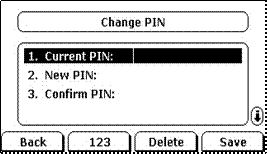
\includegraphics[width=1.33911in,height=0.21in]{media/image291.png}

\begin{quote}
To edit a contact in the local directory:
\end{quote}

\begin{enumerate}
\def\labelenumi{\arabic{enumi}.}
\item
Press the Directory soft key.
\end{enumerate}

\begin{quote}
The IP phone enters the local directory directly as there is only Local
Directory enabled in the directory by default.

If Local Directory is removed from the directory, press
Menu-\textgreater Directory-\textgreater Local Directory to enter the
local directory.
\end{quote}

\begin{enumerate}
\def\labelenumi{\arabic{enumi}.}
\setcounter{enumi}{1}
\item
Press the Enter soft key.
\end{enumerate}

\begin{quote}
If the groups have been added to the local directory, select the desired
group and then press the Enter soft key.
\end{quote}

\begin{enumerate}
\def\labelenumi{\arabic{enumi}.}
\setcounter{enumi}{2}
\item
Press or to select the desired contact.
\item
Press the Option soft key, and then select Detail from the prompt
list.
\end{enumerate}

Press

or

to

select

the contact information and then edit.

\begin{quote}
5.
\end{quote}

6. Press the Save soft key to accept change or the Back soft key to
cancel.


\includegraphics[width=1.45125in,height=0.21in]{media/image294.png}

\begin{quote}
To delete a contact from the local directory:
\end{quote}

\begin{enumerate}
\def\labelenumi{\arabic{enumi}.}
\item
Press the Directory soft key.
\end{enumerate}

\begin{quote}
The IP phone enters the local directory directly as there is only Local
Directory enabled in the directory by default.

If Local Directory is removed from the directory, press
Menu-\textgreater Directory-\textgreater Local Directory to enter the
local directory.
\end{quote}

\begin{enumerate}
\def\labelenumi{\arabic{enumi}.}
\setcounter{enumi}{1}
\item
Press the Enter soft key.
\end{enumerate}

\begin{quote}
If the groups have been added to the local directory, select the desired
group and then press the Enter soft key.
\end{quote}

\begin{enumerate}
\def\labelenumi{\arabic{enumi}.}
\setcounter{enumi}{2}
\item
Press or to select the desired contact.
\item
Press the Option soft key, and then select Delete from the prompt
list.
\end{enumerate}

\begin{quote}
The LCD screen prompts ``Delete selected item?''.
\end{quote}

\begin{enumerate}
\def\labelenumi{\arabic{enumi}.}
\setcounter{enumi}{4}
\item
Press the OK soft key to confirm the deletion or the Cancel soft key
to cancel.
\end{enumerate}


\includegraphics[width=1.94208in,height=0.21in]{media/image297.png}

\begin{quote}
To place a call to a contact from the local directory:
\end{quote}

\begin{enumerate}
\def\labelenumi{\arabic{enumi}.}
\item
Press the Directory soft key.
\end{enumerate}

\begin{quote}
The IP phone enters the local directory directly as there is only Local
Directory enabled in the directory by default.

If Local Directory is removed from the directory, press
Menu-\textgreater Directory-\textgreater Local Directory to enter the
local directory.
\end{quote}

\begin{enumerate}
\def\labelenumi{\arabic{enumi}.}
\setcounter{enumi}{1}
\item
Press the Enter soft key.
\end{enumerate}

\begin{quote}
If the groups have been added to the local directory, select the desired
group and then press the Enter soft key.
\end{quote}

\begin{enumerate}
\def\labelenumi{\arabic{enumi}.}
\setcounter{enumi}{2}
\item
Press or to select the desired contact.
\item
Do one of the following:

\begin{itemize}
\item
If only one number for the contact is stored in the local directory,
press the Send soft key to dial out the number.
\item
If multiple numbers for the contact are stored in the local
directory, press the Send soft key to display a list of numbers.
\end{itemize}
\end{enumerate}

\begin{quote}
Press or to select the desired number.

Press the Send soft key to dial out the number.
\end{quote}


\includegraphics[width=1.81278in,height=0.21in]{media/image298.png}

\begin{quote}
To search for a contact in the local directory:
\end{quote}

\begin{enumerate}
\def\labelenumi{\arabic{enumi}.}
\item
Press the Directory soft key.
\end{enumerate}

\begin{quote}
The IP phone enters the local directory directly as there is only Local
Directory enabled in the directory by default.

If Local Directory is removed from the directory, press
Menu-\textgreater Directory-\textgreater Local Directory to enter the
local directory.
\end{quote}

\begin{enumerate}
\def\labelenumi{\arabic{enumi}.}
\setcounter{enumi}{1}
\item
Press or to select the All Contacts field.
\item
Press the Search soft key.
\item
Enter a few continuous characters of the contact name or continuous
numbers of the contact number (office number, mobile number or other
number) using the keypad.
\end{enumerate}

\begin{quote}
The contacts whose name or phone number matches the characters entered
will appear on the LCD screen. You can dial from the result list.
\end{quote}

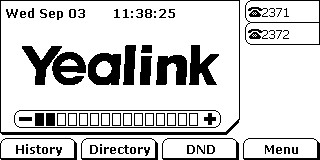
\includegraphics[width=2.23514in,height=0.21in]{media/image301.png}

\begin{quote}
You can search for a contact in your desired lists when the phone is in
the dialing screen.

The lists may contain Local Directory, History, Remote Phone Book and
LDAP.

To configure search source list in dialing via web user interface:
\end{quote}

\begin{enumerate}
\def\labelenumi{\arabic{enumi}.}
\item
Click on Directory-\textgreater Setting.
\item
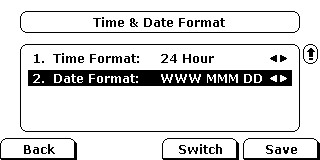
\includegraphics[width=0.21358in,height=0.15625in]{media/image262.png}In
the Search Source List In Dialing block, select the desired list from
the Disabled column and then click .
\end{enumerate}

\begin{quote}
The selected list appears in the Enabled column.
\end{quote}

\begin{enumerate}
\def\labelenumi{\arabic{enumi}.}
\setcounter{enumi}{2}
\item
Repeat step 2 to add more lists to the Enabled column.
\item
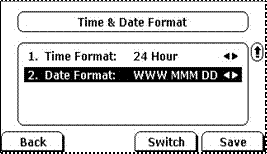
\includegraphics[width=0.21414in,height=0.15972in]{media/image263.png}To
remove a list from the Enabled column, select the desired list and
then click .
\item

\includegraphics[width=0.21414in,height=0.15972in]{media/image264.png}
\includegraphics[width=0.21414in,height=0.15972in]{media/image265.png}To
adjust the display order of search results, select the desired list
and then click or .
\end{enumerate}

\begin{quote}
The LCD screen will display search results in the adjusted order.
\end{quote}

\begin{enumerate}
\def\labelenumi{\arabic{enumi}.}
\setcounter{enumi}{5}
\item
Click Confirm to accept the change.
\end{enumerate}

%\begin{longtable}[]{@{}
%>{\raggedright\arraybackslash}p{(\linewidth - 0\tabcolsep) * \real{1.0000}}@{}}
%\toprule\noalign{}
\begin{minipage}[b]{\linewidth}\raggedright
Search source list in dialing is configurable via web user interface
only.
\end{minipage} \\
%\midrule\noalign{}
%\endhead
%\bottomrule\noalign{}
%\endlastfoot
%\end{longtable}

Note

\begin{quote}
To search for a contact in the enabled search source lists:
\end{quote}

\begin{enumerate}
\def\labelenumi{\arabic{enumi}.}
\item
Pick up the handset, press the speakerphone or press the line key.
\item
Enter a few continuous characters of the contact name or continuous
numbers of the contact number (office number, mobile number or other
number) using the keypad.
\end{enumerate}

\begin{quote}
The contacts in the enabled search source lists whose name or phone
number matches the characters entered will appear on the LCD screen. You
can press

\includegraphics[width=0.21528in,height=0.21528in]{media/image077.png} or

\includegraphics[width=0.21528in,height=0.21528in]{media/image078.png} to
scroll to the desired contact and then place a call to the contact.

You can manage your phone's local directory via phone or web user
interface. But you can only import or export the contact list via web
user interface.

To import an XML contact list file via web user interface:
\end{quote}

\begin{enumerate}
\def\labelenumi{\arabic{enumi}.}
\item
Click on Directory-\textgreater Local Directory.
\item
Click Browse to locate a contact list file (the file format must be
*.xml) from your local system.
\item
Click Import XML to import the contact list.
\end{enumerate}

\begin{quote}
The web user interface prompts "The original contact will be covered,
Continue?".
\end{quote}

\begin{enumerate}
\def\labelenumi{\arabic{enumi}.}
\setcounter{enumi}{3}
\item
Click OK to complete importing the contact list.
\end{enumerate}

\begin{quote}
To import a CSV contact list file via web user interface:
\end{quote}

\begin{enumerate}
\def\labelenumi{\arabic{enumi}.}
\item
Click on Directory-\textgreater Local Directory.
\item
Click Browse to locate a contact list file (the file format must be
*.csv) from your local system.
\item
(Optional.) Check the Show Title checkbox.
\end{enumerate}

\begin{quote}
It will prevent importing the title of the contact information which is
located in the first line of the CSV file.
\end{quote}

\begin{enumerate}
\def\labelenumi{\arabic{enumi}.}
\setcounter{enumi}{3}
\item
Click Import CSV to import the contact list.
\item
(Optional.) Mark the On radio box in the Delete Old Contacts field.
\end{enumerate}

\begin{quote}
It will delete all existing contacts while importing the contact list.
\end{quote}

\begin{enumerate}
\def\labelenumi{\arabic{enumi}.}
\setcounter{enumi}{5}
\item
Select the contact information you want to import into the local
directory from the pull down list of Index.
\end{enumerate}

\begin{quote}
At least one item should be selected to be imported into the local
directory.
\end{quote}

\begin{enumerate}
\def\labelenumi{\arabic{enumi}.}
\setcounter{enumi}{6}
\item
Click Import to complete importing the contact list.
\end{enumerate}

\begin{quote}
To export a contact list via web user interface:
\end{quote}

\begin{enumerate}
\def\labelenumi{\arabic{enumi}.}
\item
Click on Directory-\textgreater Local Directory.
\item
Click Export XML (or Export CSV).
\item
Click Save to save the contact list to your local system.
\end{enumerate}

%\begin{longtable}[]{@{}
%>{\raggedright\arraybackslash}p{(\linewidth - 0\tabcolsep) * \real{1.0000}}@{}}
%\toprule\noalign{}
\begin{minipage}[b]{\linewidth}\raggedright
Contact lists can be imported/exported via web user interface only.
\end{minipage} \\
%\midrule\noalign{}
%\endhead
%\bottomrule\noalign{}
%\endlastfoot
%\end{longtable}

Note


\includegraphics[width=0.83371in,height=0.24333in]{media/image318.png}

\begin{quote}
The built-in phone directory can store names and phone numbers for a
blacklist. You can store up to 30 contacts, add, edit, delete or search
for a contact in the blacklist directory, and even call a contact from
the blacklist directory. Incoming calls from blacklist directory
contacts will be rejected automatically.

To add a contact to the blacklist manually:
\end{quote}

\begin{enumerate}
\def\labelenumi{\arabic{enumi}.}
\item
Press Menu-\textgreater Directory-\textgreater Blacklist.
\item
Press the Add soft key.
\item
Enter the name and the office, mobile or other numbers in the
corresponding fields.
\end{enumerate}

Press or , or the

Switch

soft key to select the desired account from the

\begin{quote}
4.

Account field.

If Auto is selected, the phone will use the first available account when
placing calls to the contact from the blacklist.
\end{quote}

5. Press the Add soft key to accept the change or the Back soft key to
cancel.

\begin{quote}
To add a contact to the blacklist from the local directory:
\end{quote}

\begin{enumerate}
\def\labelenumi{\arabic{enumi}.}
\item
Press the Directory soft key.
\end{enumerate}

\begin{quote}
The IP phone enters the local directory directly as there is only Local
Directory enabled in the directory by default.

If Local Directory is removed from the directory, press
Menu-\textgreater Directory-\textgreater Local Directory to enter the
local directory.
\end{quote}

\begin{enumerate}
\def\labelenumi{\arabic{enumi}.}
\setcounter{enumi}{1}
\item
Press the Enter soft key.
\end{enumerate}

\begin{quote}
If the groups have been added to the local directory, select the desired
group and then press the Enter soft key.
\end{quote}

\begin{enumerate}
\def\labelenumi{\arabic{enumi}.}
\setcounter{enumi}{2}
\item
Press or to select the desired contact.
\item
Press the Option soft key and then select Add to Blacklist from the
prompt list.
\end{enumerate}

\begin{quote}
The LCD screen prompts "Move selected to blacklist?".
\end{quote}

\begin{enumerate}
\def\labelenumi{\arabic{enumi}.}
\setcounter{enumi}{4}
\item
Press the Ok soft key to confirm the setting.
\end{enumerate}

\begin{quote}
For more operating instructions on editing, deleting, placing calls to
and/or searching for contacts in the blacklist, refer to the operating
instructions of Local Directory on page

33.

You can add new contacts to the local directory, search for a contact,
or simply dial a contact number from the remote phone book.

You can configure your new phone to access up to 5 remote phone books.
The phone supports up to 2500 remote phone book entries. For the access
URL of the remote phone book, contact your system administrator.

To configure an access URL for a remote phone book via web user
interface:
\end{quote}

\begin{enumerate}
\def\labelenumi{\arabic{enumi}.}
\item
Click on Directory-\textgreater Remote Phone Book.
\item
Enter the access URL in the Remote URL field.
\item
Enter the name in the Display Name field.
\end{enumerate}

4.

Click

Confirm

to

accept

the

change

.

%\begin{longtable}[]{@{}
%>{\raggedright\arraybackslash}p{(\linewidth - 0\tabcolsep) * \real{1.0000}}@{}}
%\toprule\noalign{}
\begin{minipage}[b]{\linewidth}\raggedright
An access URL for a remote phone book is configurable via web user
interface only.
\end{minipage} \\
%\midrule\noalign{}
%\endhead
%\bottomrule\noalign{}
%\endlastfoot
%\end{longtable}

Note

\begin{quote}
To access your remote phone book via phone user interface:
\end{quote}

\begin{enumerate}
\def\labelenumi{\arabic{enumi}.}
\item
Press Menu-\textgreater Directory-\textgreater Remote Phone Book.
\end{enumerate}

\begin{quote}
If Remote Phone Book is added to the directory, press
Directory-\textgreater Remote Phone Book to enter the remote phone book.
\end{quote}

\begin{enumerate}
\def\labelenumi{\arabic{enumi}.}
\setcounter{enumi}{1}
\item
Select the desired remote group, and then press the Enter soft key.
\end{enumerate}

\begin{quote}
The phone then connects to the remote phone book and proceeds to load
it. The contacts in the remote phone book are displayed on the LCD
screen.
\end{quote}

\begin{enumerate}
\def\labelenumi{\arabic{enumi}.}
\setcounter{enumi}{2}
\item
Press the Back soft key to back to the previous interface.
\end{enumerate}

\begin{quote}
To search for a contact in the remote phone book:
\end{quote}

\begin{enumerate}
\def\labelenumi{\arabic{enumi}.}
\item
Press Menu-\textgreater Directory-\textgreater Remote Phone Book.
\end{enumerate}

\begin{quote}
If Remote Phone Book is added to the directory, press
Directory-\textgreater Remote Phone Book to enter the remote phone book.
\end{quote}

\begin{enumerate}
\def\labelenumi{\arabic{enumi}.}
\setcounter{enumi}{1}
\item
Select the desired remote group, and then press the Enter soft key to
load the remote phone book.
\item
Press the Search soft key.
\item
Enter a few continuous characters of the contact name or continuous
numbers of the contact number using the keypad.
\end{enumerate}

\begin{quote}
The contacts whose name or phone number matches the characters entered
will appear on the LCD screen. You can dial from the result list.

To place a call from the remote phone book:
\end{quote}

\begin{enumerate}
\def\labelenumi{\arabic{enumi}.}
\item
Press Menu-\textgreater Directory-\textgreater Remote Phone Book.
\end{enumerate}

\begin{quote}
If Remote Phone Book is added to the directory, press
Directory-\textgreater Remote Phone

Book to enter the remote phone book.
\end{quote}

\begin{enumerate}
\def\labelenumi{\arabic{enumi}.}
\setcounter{enumi}{1}
\item
Select the desired remote group, and then press the Enter soft key to
load the remote phone book.
\item
Select the desired contact in the remote phone book.
\item
Press the Send soft key.
\end{enumerate}

\begin{quote}
In addition, you can enable the phone to present the caller identify
stored in the remote phone book when receiving a call.

To enable the presentation of caller identify stored in a remote phone
book via web user interface:
\end{quote}

\begin{enumerate}
\def\labelenumi{\arabic{enumi}.}
\item
Click on Directory-\textgreater Remote Phone Book.
\item
Select Enabled from the pull-down list of Incoming/Outgoing Call
lookup.
\item
Enter the desired refresh period in the Update Time Interval (Seconds)
field.
\end{enumerate}

\begin{quote}
The default value is 21600 seconds.
\end{quote}

\begin{enumerate}
\def\labelenumi{\arabic{enumi}.}
\setcounter{enumi}{3}
\item
Click Confirm to accept the change.
\end{enumerate}

\begin{quote}
The SIP-T28P IP phone maintains call history lists of Placed Calls,
Received Calls, Missed Calls and Forwarded Calls. Call history lists
support 100 entries in all. You can view call history, place a call, add
a contact or delete an entry from the call history list.

History record feature is enabled by default. If you don't want to save
the call history, you can disable the feature.

To disable history record via phone user interface:
\end{quote}

1. Press Menu-\textgreater Features-\textgreater History Setting.

\begin{quote}
field.
\end{quote}

2.

Press

or

, or the

Switch

soft key

to select

Disable

d

from

the

History Record

3. Press the Save soft key to accept the change or the Back soft key to
cancel.

\begin{quote}
To view call history:
\end{quote}

\begin{enumerate}
\def\labelenumi{\arabic{enumi}.}
\item
Press the History soft key.
\end{enumerate}

\begin{quote}
The LCD screen displays All Calls list.
\end{quote}

\begin{enumerate}
\def\labelenumi{\arabic{enumi}.}
\setcounter{enumi}{1}
\item
Press or to switch between All Calls, Placed Calls, Received Calls,
Missed Calls and Forwarded Calls.
\item
Press or to select the desired entry.
\item
Press the Option soft key, and then select Detail from the prompt
list.
\end{enumerate}

\begin{quote}
The detailed information of the entry appears on the LCD screen.

To place a call from the call history list:
\end{quote}

\begin{enumerate}
\def\labelenumi{\arabic{enumi}.}
\item
Press the History soft key.
\item
Press or to switch between All Calls, Placed Calls, Received Calls,
Missed Calls and Forwarded Calls.
\item
Press or to select the desired entry.
\item
Press the Send soft key.
\end{enumerate}

\begin{quote}
To add a contact to the local directory or blacklist from the call
history list:
\end{quote}

\begin{enumerate}
\def\labelenumi{\arabic{enumi}.}
\item
Press the History soft key.
\item
Press or to switch between All Calls, Placed Calls, Received Calls,
Missed Calls and Forwarded Calls.
\item
Press or to select the desired entry.
\item
Press the Option soft key, and then select Add to Contacts (or Add to
Blacklist) from the prompt list.
\item
Enter the desired values in the corresponding fields, and then press
the Save soft key.
\end{enumerate}

\begin{quote}
For more information, refer to Contact Management on page 31.

To delete an entry from the call history list:
\end{quote}

\begin{enumerate}
\def\labelenumi{\arabic{enumi}.}
\item
Press the History soft key.
\item
Press or to switch between All Calls, Placed Calls, Received Calls,
Missed Calls and Forwarded Calls.
\item
Press or to select the desired entry.
\item
Press the Delete soft key.
\end{enumerate}

\begin{quote}
To delete all entries from the call history list:
\end{quote}

\begin{enumerate}
\def\labelenumi{\arabic{enumi}.}
\item
Press the History soft key.
\item
Press or to switch between All Calls, Placed Calls, Received Calls,
Missed Calls and Forwarded Calls
\item
Press the Option soft key, and then select Delete All from the prompt
list.
\item
Press the OK soft key.
\end{enumerate}

\begin{quote}
The LCD screen prompts "Delete all the call records?".
\end{quote}

\begin{enumerate}
\def\labelenumi{\arabic{enumi}.}
\setcounter{enumi}{4}
\item
Press the OK soft key to confirm the deletion or the Cancel soft key
to cancel.
\end{enumerate}


\includegraphics[width=2.49792in,height=0.28in]{media/image341.png}


\includegraphics[width=1.89361in,height=0.24333in]{media/image342.png}

\begin{quote}
You can upload your custom logo which will be displayed on the idle
screen.

To upload a custom logo via web user interface:
\end{quote}

\begin{enumerate}
\def\labelenumi{\arabic{enumi}.}
\item
Click on Features-\textgreater General Information.
\item
Select Custom logo from the pull-down list of Use Logo.
\item
Click Browse to locate the logo file from your local system.
\item
Click Upload to upload the file.
\item
Click Confirm to accept the change.
\end{enumerate}

%\begin{longtable}[]{@{}
%>{\raggedright\arraybackslash}p{(\linewidth - 0\tabcolsep) * \real{1.0000}}@{}}
%\toprule\noalign{}
\begin{minipage}[b]{\linewidth}\raggedright
The logo file format must be *.dob, contact your system administrator
for more information.

A custom logo can be uploaded via web user interface only.
\end{minipage} \\
%\midrule\noalign{}
%\endhead
%\bottomrule\noalign{}
%\endlastfoot
%\end{longtable}

Note

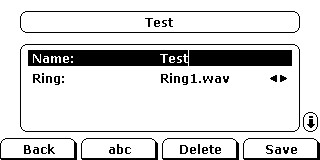
\includegraphics[width=1.21128in,height=0.24333in]{media/image345.png}

\begin{quote}
Physically connect your headset and activate the headset mode for use.
For more information on physically connecting a headset, refer to Phone
Installation on page 11

To activate the headset mode:
\end{quote}

1. Press

\includegraphics[width=0.29508in,height=0.21458in]{media/image352.png}
on the phone.

\begin{quote}
The HEADSET key LED illuminates solid green when the headset mode is
activated. Press the line key or the Answer soft key to answer a call.
The call will connect to your headset automatically. Enter the desired
number and press the Send soft key, the phone will then place a call
using the headset automatically. For more information on using the
headset to place a call, refer to Placing Calls on page 73.

To deactivate the headset mode:
\end{quote}

1. Press

\includegraphics[width=0.29508in,height=0.21458in]{media/image352.png}
again on the phone.

\begin{quote}
The HEADSET key LED goes out when the headset mode is deactivated.
\end{quote}

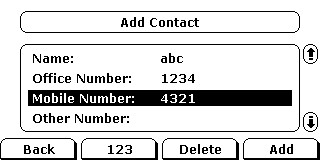
\includegraphics[width=1.12394in,height=0.21in]{media/image353.png}

\begin{quote}
You can use headset in priority when headset prior feature is enabled.
This feature is especially useful for permanent or full-time headset
users.

To enable headset prior via web user interface:
\end{quote}

\begin{enumerate}
\def\labelenumi{\arabic{enumi}.}
\item
Click on Features-\textgreater General Information.
\item
Select Enabled from the pull-down list of Headset Prior.
\item
Click Confirm to accept the change.
\end{enumerate}

\begin{quote}
To use headset prior, you should activate the headset mode in advance:
\end{quote}

\begin{enumerate}
\def\labelenumi{\arabic{enumi}.}
\item
Physically connect the headset.
\item
Press

\includegraphics[width=0.292in,height=0.21597in]{media/image352.png}
to activate the headset mode.
\end{enumerate}

%\begin{longtable}[]{@{}
%>{\raggedright\arraybackslash}p{(\linewidth - 0\tabcolsep) * \real{1.0000}}@{}}
%\toprule\noalign{}
\begin{minipage}[b]{\linewidth}\raggedright
If headset prior is enabled, the headset mode will not be deactivated
until you press the HEADSET key again.

If headset prior is disabled, the headset mode can be deactivated by
pressing the speakerphone key or the HEADSET key.

Headset prior is configurable via web user interface only.
\end{minipage} \\
%\midrule\noalign{}
%\endhead
%\bottomrule\noalign{}
%\endlastfoot
%\end{longtable}

Note


\includegraphics[width=1.11258in,height=0.21in]{media/image356.png}

\begin{quote}
You can use two headsets when dual headset feature is enabled. To use
this feature, you must physically connect headsets to the headset jack
and handset jack respectively. Once the phone connects to a call, the
headset connected to the headset jack will have full-duplex
capabilities, while the one connected to the handset jack will only be
able to listen.

To enable dual headset via web user interface:
\end{quote}

\begin{enumerate}
\def\labelenumi{\arabic{enumi}.}
\item
Click on Features-\textgreater General Information.
\item
Select Enabled from the pull-down list of Dual-Headset.
\item
Click Confirm to accept the change.
\end{enumerate}

%\begin{longtable}[]{@{}
%>{\raggedright\arraybackslash}p{(\linewidth - 0\tabcolsep) * \real{1.0000}}@{}}
%\toprule\noalign{}
\begin{minipage}[b]{\linewidth}\raggedright
Dual headset is configurable via web user interface only.
\end{minipage} \\
%\midrule\noalign{}
%\endhead
%\bottomrule\noalign{}
%\endlastfoot
%\end{longtable}

Note


\includegraphics[width=0.91163in,height=0.24333in]{media/image359.png}

\begin{quote}
There are four types of DSS keys: Memory Keys, Line Keys, Programmable
Keys and Ext Keys. The details will be introduced in the following. The
use of line keys and memory keys are almost the same. The SIP-T28P IP
phone supports 10 memory keys and 6 line keys.
\end{quote}


\includegraphics[width=1.12764in,height=0.21in]{media/image360.png}

\begin{quote}
You can assign predefined functionalities to the memory keys located on
the right of the phone. Memory keys allow you to have quick access to
features such as recall and voice mail. The memory key LEDs will
indicate status when the keys are assigned with particular features,
such as BLF. The default key type of each memory key is N/A, which
indicates that this memory key provides no functionality until
configuration.

To configure a memory key via phone user interface:
\end{quote}

\begin{enumerate}
\def\labelenumi{\arabic{enumi}.}
\item
Press Menu-\textgreater Features-\textgreater DSS
Keys-\textgreater Memory Keys.
\item
Select the desired memory key, and then press the Enter soft key.
\item
Select the desired key type from the Type field.
\item
(Optional.) Select the desired key event type from the Key Type field.
\item
(Optional.) Select the desired account from the Account ID field.
\item
(Optional.) Enter the corresponding value in the Value field.
\item
(Optional.) Enter the corresponding value in the Extension field.
\item
Press the Save soft key to accept the change or the Back soft key to
cancel.
\end{enumerate}

\begin{quote}
Memory key is configurable via web user interface at the path
DSSKey-\textgreater Memory Key.
\end{quote}

%\begin{longtable}[]{@{}
%>{\raggedright\arraybackslash}p{(\linewidth - 0\tabcolsep) * \real{1.0000}}@{}}
%\toprule\noalign{}
\begin{minipage}[b]{\linewidth}\raggedright
When the phone is idle, you can also long press the memory key to
configure it directly on the phone.
\end{minipage} \\
%\midrule\noalign{}
%\endhead
%\bottomrule\noalign{}
%\endlastfoot
%\end{longtable}

Note

\begin{quote}
Common used memory key features are explained in the following
subchapters in detail:
\end{quote}

\begin{itemize}
\item
Line
\item
Speed Dial
\item
Voice Mail
\item
Directed Pickup
\item
Group Pickup
\item
DTMF
\item
Prefix
\item
Local Group
\item
XML Group
\item
XML Browser
\item
LDAP
\item
Conference
\item
Forward
\item
Transfer
\item
Hold
\item
DND
\item
SMS
\item
Group Listening
\item
Zero Touch
\item
URL
\item
Phone Lock
\item
Directory
\end{itemize}

\begin{quote}
For the features not listed above, refer to Basic Call Features on page
73 and Advanced Phone Features on page 109. For more information,
contact your system administrator.

Line

You can use this key feature to accept incoming calls, place active
calls on hold or resume a held call. It performs in the same way as a
hard line key.

Dependencies: Type (Line)

Account ID (the account this feature will be applied to)

Label (key label displayed on the LCD screen) Usage: When receiving an
incoming call, the DSS key LED flashes green:
\end{quote}

\begin{enumerate}
\def\labelenumi{\arabic{enumi}.}
\item
Press the DSS key to accept the incoming call.
\item
Press the DSS key to place a new call.
\end{enumerate}

\begin{quote}
The active call is placed on hold.
\end{quote}

\begin{enumerate}
\def\labelenumi{\arabic{enumi}.}
\setcounter{enumi}{2}
\item
Press the DSS key to cancel the new call.
\item
Press the DSS key again to resume the held call.
\end{enumerate}

\begin{quote}
Speed Dial

You can use this key feature to speed up dialing the numbers frequently
used or hard to remember.

Dependencies: Type (Speed Dial)

Account ID (the account this feature will be applied to)

Value (the number you want to dial out)

Usage: Press the DSS key to dial out the number specified in the Value
field, using the account selected from the Account ID field.

Voice Mail

You can use this key feature to quickly connect voice mail. For more
information, refer to Voice Mail on page 129.

Dependencies: Type (Key Event)

Key Type (Voice Mail)

Account ID (the account this feature will be applied to)

Value (the voice mail access code)

Usage: Press the DSS key to dial out the voice mail access code. Then
follow the voice prompt to listen to voice mails.

Directed Pickup

You can use this key feature to answer someone else's incoming call on
the phone.

Dependencies: Type (Key Event)

Key Type (DPickup)

Account ID (the account this feature will be applied to)

Value (the directed pickup code followed by the target phone number)

Usage: Press the DSS key on your phone when the target phone number
receives an incoming call. The call is then answered on your phone.

Group Pickup

You can use this key feature to answer incoming calls in a group that is
associated with their own group.

Dependencies: Type (Key Event)

Key Type (GPickup)

Account ID (the account this feature will be applied to)

Value (the group pickup feature code)

Usage: Press the DSS key on your phone when a phone number in the group
receives an incoming call. The call is answered on your phone.

DTMF

You can use this key feature to send the specification of arbitrary key
sequences via DTMF.

Dependencies: Type (Key Event)

Key Type (DTMF)

Value (DTMF sequence)
\end{quote}

%\begin{longtable}[]{@{}
%>{\raggedright\arraybackslash}p{(\linewidth - 0\tabcolsep) * \real{1.0000}}@{}}
%\toprule\noalign{}
\begin{minipage}[b]{\linewidth}\raggedright
DTMF sequence only contains "0-9", "*", "\#" and "A-D".
\end{minipage} \\
%\midrule\noalign{}
%\endhead
%\bottomrule\noalign{}
%\endlastfoot
%\end{longtable}

Note

\begin{quote}
Usage: Press the DSS key during an active call to send the key sequence
specified in the Value field. Prefix

You can use this key feature to add a specified prefix number before the
dialed number.

Dependencies: Type (Key Event)

Key Type (Prefix)

Value (the prefix number)

Usage: Press the DSS key when the phone is idle, the phone will then
enter the pre-dialing screen and display the prefix number that you
specified in the Value field.

You can enter the remaining digits.

Local Group

You can use this key feature to quickly access a group in the local
directory. For more information, refer to Local Directory on page 33.

Dependencies: Type (Key Event)

Key Type (Local Group)
\end{quote}

%\subsubsection{\texorpdfstring{Local Group (the group you want to
%access)
%}{Local Group (the group you want to access) }}\label{local-group-the-group-you-want-to-access}

\begin{quote}
Usage: Press the DSS key to access the group specified in the Local
Group field.

XML Group

You can use this key feature to quickly access a remote group in your
remote phone book. You should configure a remote phone book in advance.
For more information, refer to Remote Phone Book on page 46.

Dependencies: Type (Key Event)

Key Type (XML Group)

Phone Book Name (the remote group you want to access if the remote phone
book is configured)

Usage: Press the DSS key to access the remote group specified in the
Phone Book Name field.

XML Browser

You can use this key feature to quickly access a XML browser. The XML
browser allows you to create custom services which meet your functional
requirements on the server.

You can customize practical applications, such as weather report, stock
information, Google search, etc.

Dependencies: Type (XML Browser)

Value (the access URL for xml browser)

Usage: Press the DSS key to access the XML browser specified in the
Value field.

LDAP

You can use this key feature to quickly access a LDAP search screen.

Dependencies: Type (Key Event)

Key Type (LDAP)

Usage:
\end{quote}

\begin{enumerate}
\def\labelenumi{\arabic{enumi}.}
\item
Press the DSS key to access the LDAP search screen.
\item
Enter a few continuous characters of the contact name or continuous
numbers of the contact number using the keypad.
\end{enumerate}

\begin{quote}
The contacts whose name or phone number matches the characters entered
will appear on the LCD screen.

Conference

You can use this key feature to set up a conference call. For more
information, refer to Conference on page 97.

Dependencies: Type (Key Event)

Key Type (Conf)

Value (the number you want to add to the conference)

Usage: Press the DSS key during an active call to set up a conference
with the number specified in the Value field.
\end{quote}

%\begin{longtable}[]{@{}
%>{\raggedright\arraybackslash}p{(\linewidth - 0\tabcolsep) * \real{1.0000}}@{}}
%\toprule\noalign{}
\begin{minipage}[b]{\linewidth}\raggedright
If the Value field is left blank, the DSS key performs the same function
as the CONF key or the Conf soft key during a call.
\end{minipage} \\
%\midrule\noalign{}
%\endhead
%\bottomrule\noalign{}
%\endlastfoot
%\end{longtable}

Note

\begin{quote}
Forward

You can use this key feature to forward an incoming call to someone
else. For more information, refer to Call Forward on page 88.

Dependencies: Type (Key Event)

Key Type (Forward)

Value (the number you want to forward to)

Usage: Press the DSS key to forward an incoming call to the number
specified in the Value field.
\end{quote}

Note If the Value field is left blank, the DSS key performs the same
function as the Forward soft key when receiving an incoming call.

\begin{quote}
Transfer

When there is an active call on the phone, you can use this key feature
to handle the call differently depending on the transfer mode assigned
to the DSS key.

Dependencies: Type (Key Event)

Key Type (Transfer)

Value (the number you want to transfer to)

Usage:
\end{quote}

\begin{itemize}
\item
When the transfer mode on DSS key is Blind Transfer, press the DSS key
to complete the blind transfer to the number specified in the Value
field.
\item
When the transfer mode on DSS key is Attended Transfer, press the DSS
key to dial out the number specified in the Value field, and then you
can perform the attended or semi-attended transfer.
\item
When the transfer mode on DSS key is New Call, press the DSS key to
place a new call to the number specified in the Value field.
\end{itemize}

\begin{quote}
Note Transfer mode on DSS key is configurable via web user interface at
the path Features-\textgreater Transfer-\textgreater Transfer Mode Via
Dsskey.

If the Value field is left blank, the DSS key performs the same function
as the TRAN key or the Transfer soft key during a call. For more
information, refer to Call Transfer on page 95.

Hold

You can use this key feature to place an active call on hold or retrieve
a held call.

Dependencies: Type (Key Event)

Key Type (Hold)

Usage:
\end{quote}

\begin{enumerate}
\def\labelenumi{\arabic{enumi}.}
\item
Press the DSS key during an active call to place the call on hold.
\item
Press the DSS key again to retrieve the held call.
\end{enumerate}

\begin{quote}
DND

You can use this key feature to activate or deactivate DND. You can also
use this key feature to access the custom DND screen. For more
information, refer to Do Not Disturb (DND) on page 84.

Dependencies: Type (Key Event)

Key Type (DND)

Usage:

When the DND is in phone mode:
\end{quote}

\begin{enumerate}
\def\labelenumi{\arabic{enumi}.}
\item
Press the DSS key to activate DND.
\item
Press the DSS key again to deactivate DND.
\end{enumerate}

\begin{quote}
When the DND is in custom mode:
\end{quote}

\begin{enumerate}
\def\labelenumi{\arabic{enumi}.}
\item
Press the DSS key to access the custom DND screen.
\item
Activate or deactivate DND for an account or all accounts.
\end{enumerate}

%\begin{longtable}[]{@{}
%>{\raggedright\arraybackslash}p{(\linewidth - 0\tabcolsep) * \real{1.0000}}@{}}
%\toprule\noalign{}
\begin{minipage}[b]{\linewidth}\raggedright
When DND is activated, the incoming calls will be rejected
automatically.
\end{minipage} \\
%\midrule\noalign{}
%\endhead
%\bottomrule\noalign{}
%\endlastfoot
%\end{longtable}

Note

\begin{quote}
SMS

You can use this key feature to quickly access text message. For more
information, refer to Short Message Service (SMS) on page 126.

Dependencies: Type (Key Event)

Key Type (SMS)

Usage: Press the DSS key when the phone is idle to access text message.

Group Listening

You can use this key feature to activate the Speakerphone and
Handset/Headset mode at the same time. It is suitable for the group
conversations which have more than one person present at one end. You
are able to speak and listen through the handset/headset, while the
others nearby can only listen through the speaker.

Dependencies: Type (Key Event)

Key Type (Group Listening)

Usage:
\end{quote}

\begin{enumerate}
\def\labelenumi{\arabic{enumi}.}
\item
During a call, press the DSS key to activate the group listening mode.
\end{enumerate}

\begin{quote}
You can then speak and listen through the handset/ headset, while other
people at your side can only listen through the speaker at the same
time.
\end{quote}

\begin{enumerate}
\def\labelenumi{\arabic{enumi}.}
\setcounter{enumi}{1}
\item
Press the DSS key again to deactivate the group listening mode.
\end{enumerate}

\begin{quote}
Zero Touch

You can use this key feature to quickly configure auto provision and
network

parameters.

Dependencies: Type (Key Event)

Key Type (Zero Touch)

Usage:
\end{quote}

\begin{enumerate}
\def\labelenumi{\arabic{enumi}.}
\item
Press the DSS key to access the zero touch screen.
\item
Press the OK soft key within a few seconds.
\item
Configure the network parameters in the corresponding fields.
\item
Press the Next soft key.
\item
Configure the auto provision parameters in the corresponding fields.
\item
Press the OK soft key.
\end{enumerate}

\begin{quote}
The phone will reboot to update configurations.

URL

You can use this key feature to trigger the phone to send an HTTP GET
request containing a specific URL.

Dependencies: Type (URL)
\end{quote}

%\subsubsection{\texorpdfstring{Value (the URL contained in the HTTP GET
%request)
%}{Value (the URL contained in the HTTP GET request) }}\label{value-the-url-contained-in-the-http-get-request}

\begin{quote}
Usage: Press the DSS key to trigger the phone to send an HTTP GET
request containing the URL specified in the Value field.

Phone Lock


\includegraphics[width=0.29167in,height=0.19792in]{media/image229.png}You
can use this key feature to immediately lock your phone instead of long
pressing . For more information, refer to Phone Lock on page 25.

Dependencies: Type (phone Lock)

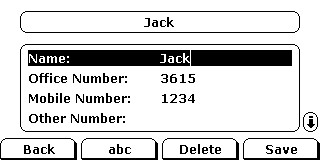
\includegraphics[width=0.29306in,height=0.19722in]{media/image361.png}Usage:
Press the DSS key to immediately lock your phone instead of long
pressing .

Directory

You can use this key feature to easily access frequently used lists. For
more information, refer to Directory on page 31.

Dependencies: Type (Directory)

Usage: Press the DSS key to immediately access frequently used lists.
\end{quote}

%\begin{longtable}[]{@{}
%>{\raggedright\arraybackslash}p{(\linewidth - 0\tabcolsep) * \real{1.0000}}@{}}
%\toprule\noalign{}
\begin{minipage}[b]{\linewidth}\raggedright
The DSS key performs the same function as the Directory soft key when
the phone is idle.
\end{minipage} \\
%\midrule\noalign{}
%\endhead
%\bottomrule\noalign{}
%\endlastfoot
%\end{longtable}

Note


\includegraphics[width=0.80038in,height=0.21in]{media/image362.png}

\begin{quote}
You can assign predefined functionalities to the line keys as same as
memory keys. You can also define a label for line key which will appear
on the LCD screen. The default key type of each line key is Line.

To configure a line key via phone user interface:
\end{quote}

\begin{enumerate}
\def\labelenumi{\arabic{enumi}.}
\item
Press Menu-\textgreater Features-\textgreater DSS
Keys-\textgreater Line Keys.
\item
Select the desired line key, and then press the Enter soft key.
\item
Select the desired key type from Type field.
\item
(Optional.) Select the desired key event type from the Key Type field.
\item
(Optional.) Select the desired account from the Account ID field.
\item
(Optional.) Enter the string that will appear on the LCD screen in the
Label field.
\item
(Optional.) Enter the corresponding value in the Value field.
\item
(Optional.) Enter the corresponding value in the Extension field.
\item
Press the Save soft key to accept the change or the Back soft key to
cancel.
\end{enumerate}

\begin{quote}
Line key is configurable via web user interface at the path
DSSKey-\textgreater Line Key.

For more information on using the line keys, refer to Memory Keys
introduced above on page 53.
\end{quote}


\includegraphics[width=1.63833in,height=0.21in]{media/image363.png}

\begin{quote}
You can customize the soft keys, navigation keys and function keys on
the keypad.

To customize programmable keys via web user interface:
\end{quote}

1. Click on DSSKey-\textgreater Programmable Key.

2.

Customize specific features for these keys.

3. Click Confirm to accept the change.

\begin{quote}
You can click Reset to default to reset custom settings to defaults.

Then you can press the keys on the phone to perform the features you
configured.

For example:

Switch Account

You can press this key to switch default account.

Dependencies: Type (Switch Account)

Usage: Press the programmable key to scroll down the account list to
select the desired default account.
\end{quote}

%\begin{longtable}[]{@{}
%>{\raggedright\arraybackslash}p{(\linewidth - 0\tabcolsep) * \real{1.0000}}@{}}
%\toprule\noalign{}
\begin{minipage}[b]{\linewidth}\raggedright
Programmable keys are configurable via web user interface only.
\end{minipage} \\
%\midrule\noalign{}
%\endhead
%\bottomrule\noalign{}
%\endlastfoot
%\end{longtable}

Note

\begin{quote}
You can customize features to Ext keys.

To customize Ext keys via web user interface:
\end{quote}

1. Click on DSSKey-\textgreater Ext Key.

2.

Customize specific features for these keys.

3. Click Confirm to accept the change.

\begin{quote}
For more information, refer to EXP39 User Guide.
\end{quote}

%\begin{longtable}[]{@{}
%>{\raggedright\arraybackslash}p{(\linewidth - 0\tabcolsep) * \real{1.0000}}@{}}
%\toprule\noalign{}
\begin{minipage}[b]{\linewidth}\raggedright
Ext keys are configurable via web user interface only.
\end{minipage} \\
%\midrule\noalign{}
%\endhead
%\bottomrule\noalign{}
%\endlastfoot
%\end{longtable}

Note


\includegraphics[width=2.09069in,height=0.24333in]{media/image372.png}

\begin{quote}
You can register one or multiple accounts on the SIP-T28P IP phone. You
can also configure each line key to associate with an account or
configure multiple line keys to associate with an account.
\end{quote}

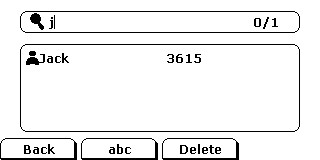
\includegraphics[width=1.69472in,height=0.21in]{media/image373.png}

\begin{quote}
To register an account via phone user interface:
\end{quote}

\begin{enumerate}
\def\labelenumi{\arabic{enumi}.}
\item
Press Menu-\textgreater Settings-\textgreater Advanced Settings
(default password: admin) -\textgreater Accounts.
\item
Select the desired account and then press the Enter soft key.
\item
Select Enabled from the Account Status field.
\item
Enter the desired values in the Label, Display Name, Register Name,
User Name, Password and SIP Server1/2 fields respectively. Contact
your system administrator for more information.
\item
Press the Save soft key to accept the change or the Back soft key to
cancel.
\end{enumerate}

\begin{quote}
You can repeat steps 2 to 5 to register more accounts.

The following figures demonstrate single or multiple accounts registered
on the phone:

Single account:

Multiple accounts:

To disable an account via phone user interface:
\end{quote}

\begin{enumerate}
\def\labelenumi{\arabic{enumi}.}
\item
Press Menu-\textgreater Settings-\textgreater Advanced Settings
(default password: admin) -\textgreater Accounts.
\item
Select the desired account and then press the Enter soft key.
\item
Select Disabled from the Account Status field.
\item
Press the Save soft key to accept the change or the Back soft key to
cancel.
\end{enumerate}

\begin{quote}
Account registration is configurable via web user interface at the path
Account-\textgreater Register.
\end{quote}

%\begin{longtable}[]{@{}
%>{\raggedright\arraybackslash}p{(\linewidth - 0\tabcolsep) * \real{1.0000}}@{}}
%\toprule\noalign{}
\begin{minipage}[b]{\linewidth}\raggedright
Press or to set the default account. It has priority when placing a
call. The phone's default account cannot be changed after reboot.
\end{minipage} \\
%\midrule\noalign{}
%\endhead
%\bottomrule\noalign{}
%\endlastfoot
%\end{longtable}

Note

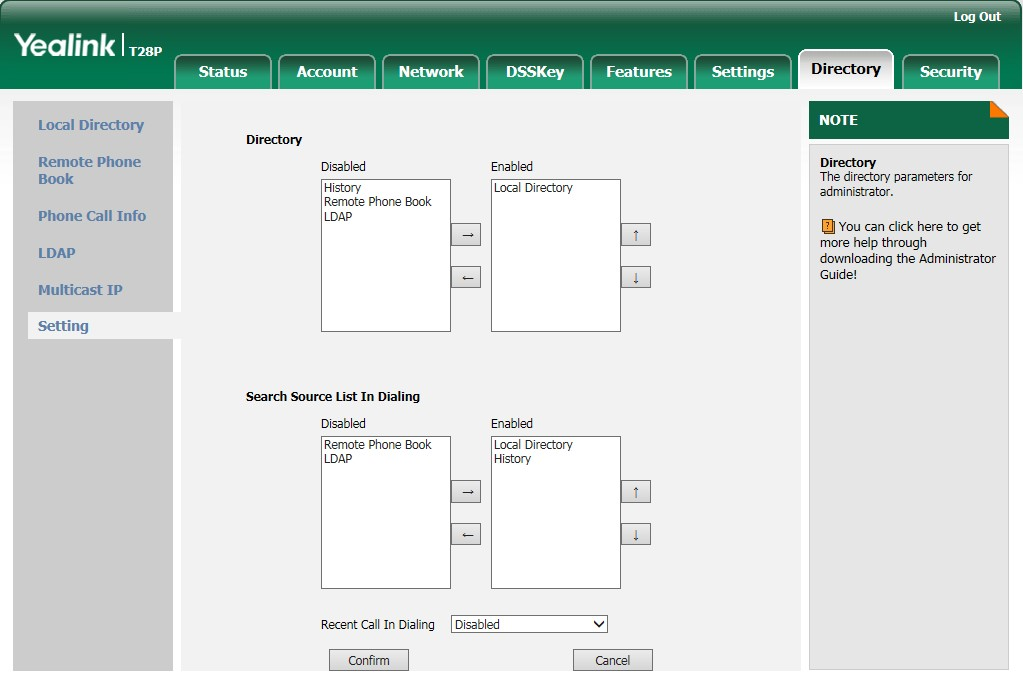
\includegraphics[width=2.44319in,height=0.21in]{media/image380.png}

\begin{quote}
You can configure multiple line keys to associate with an account. This
enhances call visualization and simplifies call handling.

If this is the case, the LCD screen will resemble the following figure:

Incoming calls to this account will be distributed evenly among the
available line keys. Outgoing calls will be distributed similarly.

Your phone can be configured to have a combination of accounts with a
single line key and accounts with multiple line keys.
\end{quote}


\includegraphics[width=0.87815in,height=0.24333in]{media/image385.png}

\begin{quote}
Dial plan is a string of characters that governs the way your SIP-T28P
IP phone processes the inputs received from your phone keypad. The
SIP-T28P IP phone supports the following dial plan features:
\end{quote}

\begin{itemize}
\item
Replace Rule
\item
Dial-now
\item
Area Code
\item
Block Out
\end{itemize}

\begin{quote}
The basic expression syntax you need to know:
\end{quote}

%\begin{longtable}[]{@{}
%>{\raggedright\arraybackslash}p{(\linewidth - 2\tabcolsep) * \real{0.0546}}
%>{\raggedright\arraybackslash}p{(\linewidth - 2\tabcolsep) * \real{0.9454}}@{}}
%\toprule\noalign{}
\begin{minipage}[b]{\linewidth}\centering
.
%\end{minipage} & \begin{minipage}[b]{\linewidth}\raggedright
The dot "." can be used as a placeholder or multiple placeholders for
any character. Example:

"12." would match "123", "1234", "12345", "12abc", etc.
\end{minipage} \\
%\midrule\noalign{}
%\endhead
%\bottomrule\noalign{}
%\endlastfoot
%\begin{minipage}[t]{\linewidth}\raggedright
\begin{quote}
x
\end{quote}
%\end{minipage} & An "x" can be used as a placeholder for any character.
Example:

"12x" would match "121", "122", "123", "12a", etc. \\
%{[}{]} & The square brackets "{[}{]}"can be used as a placeholder for a
single character which matches any of a set of characters. Example:

"91{[}5-7{]}1234" would match "9151234", "9161234", "9171234". \\
\begin{minipage}[t]{\linewidth}\raggedright
\begin{quote}
()
\end{quote}
\end{minipage} %& The parentheses "( )"can be used to group together
patterns, for instance, to logically combine two or more patterns.
Example:

``91({[}5-7{]})1(x)'' would match ``91511'', ``91618'', ``91715'',
etc. \\
\begin{minipage}[t]{\linewidth}\raggedright
\begin{quote}
\$
\end{quote}
\end{minipage} %& The ``\$'' should be followed by the sequence number of
a parenthesis. The ``\$'' plus the sequence number means the whole
character or characters placed in the parenthesis. The number directs to
the right parenthesis when there are more than one. Example:

A replace rule configuration, Prefix: "001(xxx)45(xx)", Replace:
"9001\$145\$2". When you dial out "0012354599" on your phone, the IP
phone will replace the number with "90012354599". ``\$1'' means 3 digits
in the first parenthesis, that is, ``235''. ``\$2'' means 2 digits in
the second parenthesis, that is, ``99''. \\
%\end{longtable}


\includegraphics[width=1.06564in,height=0.21in]{media/image386.png}

\begin{quote}
You can configure one or more replace rules (up to 100) to remove the
specified string and replace it with another string. You can configure a
pattern with wildcards (refer to the expression syntax in the table
above), so that any string that matches the pattern will be replaced.
This feature is convenient for you to dial out a long number. For
example, a replace rule is configured as "Prefix: 1" and "Replace:
1234", when you try to dial out the number ``1234'', you just need to
enter ``1'' on the phone and then press the Send soft key.

To add a replace rule via web user interface:
\end{quote}

\begin{enumerate}
\def\labelenumi{\arabic{enumi}.}
\item
Click on Settings-\textgreater Dial Plan-\textgreater Replace Rule.
\item
Enter the string in the Prefix field.
\item
Enter the string in the Replace field.
\item
Enter the desired line ID in the Account field or leave it blank.
\item
Click Add to add the replace rule.
\end{enumerate}

\begin{quote}
When you enter the number ``1'' using the keypad and then press the Send
soft key, the phone will dial out ``1234'' instead.

Note The valid values for the Account field can be one or more digits
among 1, 2, 3, 4, 5 and 6. Each digit must be separated by a comma. For
example, when you enter the value ``1, 2'' in the Account field, this
replace rule will apply to account1 and account2.

If you leave the Account field blank or enter 0, the replace rule will
apply to all accounts.

To edit a replace rule via web user interface:
\end{quote}

\begin{enumerate}
\def\labelenumi{\arabic{enumi}.}
\item
Click on Settings-\textgreater Dial Plan-\textgreater Replace Rule.
\item
Select the desired replace rule by checking the check box.
\item
Edit the values in the Prefix and Replace fields.
\item
Enter the desired line ID in the Account field or leave it blank.
\item
Click Edit to accept the change.
\end{enumerate}

\begin{quote}
To delete one or more replace rules via web user interface:
\end{quote}

\begin{enumerate}
\def\labelenumi{\arabic{enumi}.}
\item
Click on Settings-\textgreater Dial Plan-\textgreater Replace Rule.
\item
Select the one or more replace rules by checking the check box(es).
\item
Click Del to delete the replace rule(s).
\end{enumerate}

Note Replace rule is configurable via web user interface only.

\begin{quote}
You can configure one or more dial-now rules (up to 100) on your phone.
When the dialed out number matches the dial-now string, the number will
be dialed out automatically. For example, a dial-now rule is configured
as "2xx", any entered three-digit string beginning with 2 will then be
dialed out automatically on the phone.

To add a dial-now rule via web user interface:
\end{quote}

\begin{enumerate}
\def\labelenumi{\arabic{enumi}.}
\item
Click on Settings-\textgreater Dial Plan-\textgreater Dial-now.
\item
Enter the desired value (e.g., 2xx) in the Rule field.
\item
Enter the desired line ID in the Account field or leave it blank.
\end{enumerate}

\begin{quote}
For more information on the valid values for the Account field, refer to
Replace Rule on page 65.
\end{quote}

\begin{enumerate}
\def\labelenumi{\arabic{enumi}.}
\setcounter{enumi}{3}
\item
Click Add to add the dial-now rule.
\end{enumerate}

\begin{quote}
When you enter the number ``234'' using the keypad, the phone will dial
out ``234'' automatically without the pressing of any key.
\end{quote}

%\begin{longtable}[]{@{}
%>{\raggedright\arraybackslash}p{(\linewidth - 0\tabcolsep) * \real{1.0000}}@{}}
%\toprule\noalign{}
\begin{minipage}[b]{\linewidth}\raggedright
You can also edit or delete the dial-now rule, refer to Replace Rule on
page 65 for more information.

Dial-now rule is configurable via web user interface only.
\end{minipage} \\
%\midrule\noalign{}
%\endhead
%\bottomrule\noalign{}
%\endlastfoot
%\end{longtable}

Note

\begin{quote}
Delay Time for Dial-now Rule

You can configure the delay time for dial-now rules. That is, you can
configure your phone to automatically dial out the phone number which
matches a dial-now rule, after the designated delay time.

To configure the delay time for dial-now rule via web user interface:
\end{quote}

\begin{enumerate}
\def\labelenumi{\arabic{enumi}.}
\item
Click on Features-\textgreater General Information.
\item
Enter the time between 1 and 14 (seconds) in the Time-Out for Dial-Now
Rule field.
\item
Click Confirm to accept the change.
\end{enumerate}

%\begin{longtable}[]{@{}
%>{\raggedright\arraybackslash}p{(\linewidth - 0\tabcolsep) * \real{1.0000}}@{}}
%\toprule\noalign{}
\begin{minipage}[b]{\linewidth}\raggedright
Delay time for dial-now rule is configurable via web user interface
only.
\end{minipage} \\
%\midrule\noalign{}
%\endhead
%\bottomrule\noalign{}
%\endlastfoot
%\end{longtable}

Note


\includegraphics[width=0.87444in,height=0.21in]{media/image401.png}

\begin{quote}
Area codes are also known as Numbering Plan Areas (NPAs). They usually
indicate geographical areas in a country. This feature is necessary when
dialing a phone number outside the code area. For example, an area code
is configured as "Code: 0592, Min Length: 1, Max Length: 15". When you
dial out the number "56789" (the length of the number is between 1 and
15), the phone will add the area code and dial out the number
"059256789". You can only configure one area code rule on your phone.

To configure the area code via web user interface:
\end{quote}

\begin{enumerate}
\def\labelenumi{\arabic{enumi}.}
\item
Click on Settings-\textgreater Dial Plan-\textgreater Area Code.
\item
Enter the desired values in the Code, Min Length (1-15) and Max Length
(1-15) fields.
\item
Enter the desired line ID in the Account field or leave it blank.
\end{enumerate}

\begin{quote}
For more information on the valid values for the Account field, refer to
Replace Rule on page 65.
\end{quote}

\begin{enumerate}
\def\labelenumi{\arabic{enumi}.}
\setcounter{enumi}{3}
\item
Click Confirm to accept the change.
\end{enumerate}

%\begin{longtable}[]{@{}
%>{\raggedright\arraybackslash}p{(\linewidth - 0\tabcolsep) * \real{1.0000}}@{}}
%\toprule\noalign{}
\begin{minipage}[b]{\linewidth}\raggedright
The default values of minimum and maximum length are 1 and 15
respectively .

Area code is configurable via web user interface only.
\end{minipage} \\
%\midrule\noalign{}
%\endhead
%\bottomrule\noalign{}
%\endlastfoot
%\end{longtable}

Note


\includegraphics[width=0.8226in,height=0.21in]{media/image404.png}

\begin{quote}
You can block specific numbers from being dialed on your phone. When you
dial a block out number on your phone, the dialing will fail and the LCD
screen will prompt "Forbidden Number". You can add 10 block out rules at
most on your phone.

To add a block out number via web user interface:
\end{quote}

\begin{enumerate}
\def\labelenumi{\arabic{enumi}.}
\item
Click on Settings-\textgreater Dial Plan-\textgreater Block Out.
\item
Enter the desired value in the BlockOut Number field.
\item
Enter the desired line ID in the Account field or leave it blank.
\end{enumerate}

\begin{quote}
For more information on the valid values for the Account field, refer to
Replace Rule on page 65.
\end{quote}

\begin{enumerate}
\def\labelenumi{\arabic{enumi}.}
\setcounter{enumi}{3}
\item
Click Confirm to add the block out number.
\end{enumerate}

%\begin{longtable}[]{@{}
%>{\raggedright\arraybackslash}p{(\linewidth - 0\tabcolsep) * \real{1.0000}}@{}}
%\toprule\noalign{}
\begin{minipage}[b]{\linewidth}\raggedright
Block out number is configurable via web user interface only.
\end{minipage} \\
%\midrule\noalign{}
%\endhead
%\bottomrule\noalign{}
%\endlastfoot
%\end{longtable}

Note


\includegraphics[width=1.88847in,height=0.24333in]{media/image407.png}

\begin{quote}
Public telephone networks in countries around the world have a single
emergency telephone number (emergency services number), that allows a
caller to contact local emergency services for assistance when
necessary. The emergency telephone number may differ from country to
country. It is typically a three-digit number so that it can be easily
remembered and dialed quickly. Some countries have a different emergency
number for each of the different emergency services.

You can specify the emergency telephone numbers on the IP phone for
contacting the emergency services in an emergency situation.
\end{quote}

%\begin{longtable}[]{@{}
%>{\raggedright\arraybackslash}p{(\linewidth - 0\tabcolsep) * \real{1.0000}}@{}}
%\toprule\noalign{}
\begin{minipage}[b]{\linewidth}\raggedright
Contact your local phone service provider for available emergency
numbers in your area.
\end{minipage} \\
%\midrule\noalign{}
%\endhead
%\bottomrule\noalign{}
%\endlastfoot
%\end{longtable}

Note

\begin{quote}
To specify emergency numbers via web user interface:
\end{quote}

\begin{enumerate}
\def\labelenumi{\arabic{enumi}.}
\item
Click on Features-\textgreater Phone Lock.
\item
Enter the emergency number in the Emergency field.
\end{enumerate}

\begin{quote}
For multiple numbers, enter a comma between every two emergency numbers.
The default emergency numbers are 112, 911 and 110.
\end{quote}

\begin{enumerate}
\def\labelenumi{\arabic{enumi}.}
\setcounter{enumi}{2}
\item
Click Confirm to accept the change.
\end{enumerate}

%\begin{longtable}[]{@{}
%>{\raggedright\arraybackslash}p{(\linewidth - 0\tabcolsep) * \real{1.0000}}@{}}
%\toprule\noalign{}
\begin{minipage}[b]{\linewidth}\raggedright
Emergency number is configurable via web user interface only.
\end{minipage} \\
%\midrule\noalign{}
%\endhead
%\bottomrule\noalign{}
%\endlastfoot
%\end{longtable}

Note

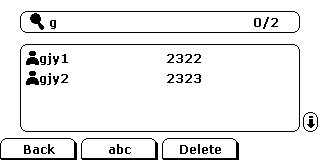
\includegraphics[width=1.20286in,height=0.24333in]{media/image410.png}

\begin{quote}
You can enable live dialpad on the SIP-T28P IP phone, which enables the
IP phone to automatically dial out a phone number without the pressing
of the send key. You can also configure a delay, where the phone will
dial out the phone number automatically after the designated period of
time.

To enable live dialpad via web user interface:
\end{quote}

\begin{enumerate}
\def\labelenumi{\arabic{enumi}.}
\item
Click on Settings-\textgreater Preference.
\item
Select Enabled from the pull-down list of Live Dialpad.
\item
Enter the desired delay time in the Inter Digit Time
(1\textasciitilde14s) field.
\end{enumerate}

The default delay time is 4s

.

\begin{enumerate}
\def\labelenumi{\arabic{enumi}.}
\setcounter{enumi}{3}
\item
Click Confirm to accept the change.
\end{enumerate}

%\begin{longtable}[]{@{}
%>{\raggedright\arraybackslash}p{(\linewidth - 0\tabcolsep) * \real{1.0000}}@{}}
%\toprule\noalign{}
\begin{minipage}[b]{\linewidth}\raggedright
Live dialpad is configurable via web user interface only.
\end{minipage} \\
%\midrule\noalign{}
%\endhead
%\bottomrule\noalign{}
%\endlastfoot
%\end{longtable}

Note

\begin{quote}
You can dial a hotline number immediately upon lifting the handset,
pressing the Speakerphone key or pressing a line key. You can also
configure a delay, where the phone will dial out the hotline number
automatically after the designated period of time.

To configure hotline number via phone user interface:
\end{quote}

\begin{enumerate}
\def\labelenumi{\arabic{enumi}.}
\item
Press Menu-\textgreater Features-\textgreater Hot Line.
\item
Enter the desired number in the Number field.
\item
Enter the delay time (in seconds) in the Hotline Delay field.
\end{enumerate}

\begin{quote}
The valid values range from 0 to 10.
\end{quote}

\begin{enumerate}
\def\labelenumi{\arabic{enumi}.}
\setcounter{enumi}{3}
\item
Press the Save soft key to accept the change or the Back soft key to
cancel.
\end{enumerate}

\begin{quote}
Hotline is configurable via web user interface at the path
Features-\textgreater General Information.

The SIP-T28P IP phone is designed to be easily used like a regular phone
on a public switched telephone network (PSTN). You can place calls,
answer calls, transfer a call to someone else, or conduct a conference
call.

This chapter provides basic operating instructions for the SIP-T28P IP
phone. Topics include:
\end{quote}

\begin{itemize}
\item
Placing Calls
\item
Answering Calls
\item
Ending Calls
\item
Redialing Numbers
\item
Recent Call In Dialing
\item
Auto Answer
\item
Auto Redial
\item
Call Completion
\item
Recall
\item
Call Mute
\item
Call Hold/Resume
\item
Do Not Disturb (DND)
\item
Call Transfer
\item
Call Waiting
\item
Conference
\item
Call Park
\item
Call Pickup
\item
Anonymous Call
\item
Anonymous Call Rejection
\end{itemize}

\begin{quote}
If you require additional information or assistance with your new phone,
contact your system administrator.
\end{quote}

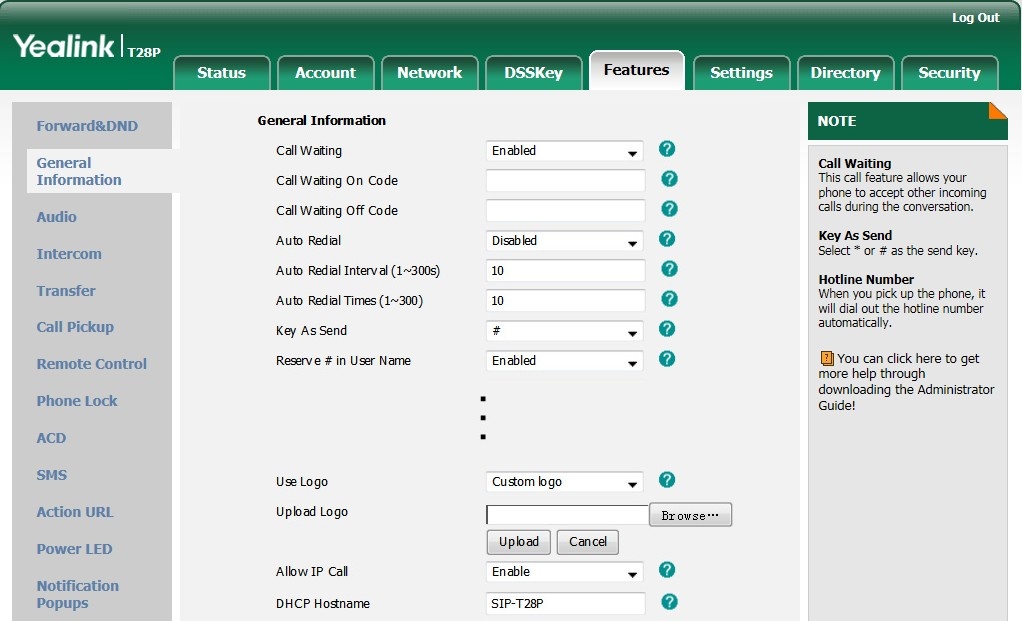
\includegraphics[width=1.37882in,height=0.28in]{media/image423.png}

\begin{quote}
You can place a call in one of three ways using your SIP-T28P IP phone:
\end{quote}

\begin{itemize}
\item
Using the handset
\item
Using the speakerphone
\item
Using the headset
\end{itemize}

\begin{quote}
You can also dial the number first, and then choose the way you want to
speak to the other party.

You can also search and dial a contact from call history, local
directory or remote phone book. For more information, refer to Contact
Management on page 31 and Call History Management on page 48.

During a call, you can alternate between Speakerphone, Headset, and
Handset modes by pressing the Speakerphone key, the HEADSET key, or by
picking up the handset.

The call duration of the active call is visible on the LCD screen. In
the figure below, the call to the number''1005'' has lasted 6 seconds.

To place a call using the handset:
\end{quote}

\begin{enumerate}
\def\labelenumi{\arabic{enumi}.}
\item
Pick up the handset.
\item
Enter the desired number using the keypad.
\item
Press , , or the Send soft key.
\end{enumerate}

\begin{quote}
The \# key is configured as a send key by default. You can also set the
* key as the send key, or set neither. For more information, refer to
Key as Send on page 24.
\end{quote}

%\begin{longtable}[]{@{}
%>{\raggedright\arraybackslash}p{(\linewidth - 0\tabcolsep) * \real{1.0000}}@{}}
%\toprule\noalign{}
\begin{minipage}[b]{\linewidth}\raggedright
You can also dial using the SIP URI or IP address. To obtain the IP
address of the phone, press the OK key when the phone is idle. The
maximum SIP URI or IP address length is 32 characters. For example, SIP
URI: 2210@sip.com, IP: 192.168.1.15.

Your phone may not support direct IP dialing. Contact your system
administrator for more information.
\end{minipage} \\
%\midrule\noalign{}
%\endhead
%\bottomrule\noalign{}
%\endlastfoot
%\end{longtable}

Note

\begin{quote}
To place a call using the hands-free speakerphone mode:

Do one of the following:
\end{quote}

\begin{itemize}
\item
With the handset on-hook, press

\includegraphics[width=0.29167in,height=0.19962in]{media/image428.png}
or the line key to obtain a dial tone.
\end{itemize}

\begin{quote}
Enter the desired number using the keypad.

Press , , or the Send soft key.
\end{quote}

\begin{itemize}
\item
With the handset on-hook, enter the desired number using the keypad.
\end{itemize}

\begin{quote}
Press , , , or the Send soft key.

To place a call using the headset:

Do one of the following:
\end{quote}

\begin{itemize}
\item
With the optional headset connected, press

\includegraphics[width=0.293in,height=0.22083in]{media/image430.png}
to activate the headset mode.
\end{itemize}

\begin{quote}
Press the line key to obtain a dial tone.

Enter the desired number using the keypad.

Press , , or the Send soft key.
\end{quote}

\begin{itemize}
\item
With the optional headset connected, press

\includegraphics[width=0.29167in,height=0.21699in]{media/image430.png}
to activate the headset mode.
\end{itemize}

\begin{quote}
Enter the desired number using the keypad.

Press , , or the Send soft key.
\end{quote}

%\begin{longtable}[]{@{}
%>{\raggedright\arraybackslash}p{(\linewidth - 0\tabcolsep) * \real{1.0000}}@{}}
%\toprule\noalign{}
\begin{minipage}[b]{\linewidth}\raggedright
To permanently activate the headset mode, refer to Headset Prior on page
51.
\end{minipage} \\
%\midrule\noalign{}
%\endhead
%\bottomrule\noalign{}
%\endlastfoot
%\end{longtable}

Note

\begin{quote}
The SIP-T28P IP phone can handle multiple calls at a time. However, only
one active call

(the call that has audio associated with it) can be in progress at any
given time. The SIP-T28P IP phone can handle a maximum of 6 calls at one
time.

To place multiple calls:

You can have more than one call on your SIP-T28P IP phone. To place a
new call during an active call, do one of the following:
\end{quote}

\begin{itemize}
\item
Press the line key. The active call is placed on hold.
\end{itemize}

\begin{quote}
Enter the desired number using the keypad.

Press , , or the Send soft key.
\end{quote}

\begin{itemize}
\item
Press

\includegraphics[width=0.29167in,height=0.21875in]{media/image431.png}
or the Hold soft key to place the original call on hold.
\end{itemize}

\begin{quote}
Press the New Call soft key.

Enter the desired number using the keypad.

Press , , or the Send soft key.

You can press or to switch between the calls, and then press the Resume
soft key to retrieve the desired call.
\end{quote}

%\begin{longtable}[]{@{}
%>{\raggedright\arraybackslash}p{(\linewidth - 0\tabcolsep) * \real{1.0000}}@{}}
%\toprule\noalign{}
\begin{minipage}[b]{\linewidth}\raggedright
If multiple accounts are registered on the phone, you can first press
the desired line key in the idle screen or press the Line soft key in
the dialing screen, and then you can use the selected account to place a
call.
\end{minipage} \\
%\midrule\noalign{}
%\endhead
%\bottomrule\noalign{}
%\endlastfoot
%\end{longtable}

Note


\includegraphics[width=1.73583in,height=0.28in]{media/image432.png}

\begin{quote}
When you are not in another call, you can answer a call in one of three
ways:
\end{quote}

\begin{itemize}
\item
Using the handset
\item
Using the speakerphone
\item
Using the headset
\end{itemize}

%\begin{longtable}[]{@{}
%>{\raggedright\arraybackslash}p{(\linewidth - 0\tabcolsep) * \real{1.0000}}@{}}
%\toprule\noalign{}
\begin{minipage}[b]{\linewidth}\raggedright
You can reject incoming calls by pressing the X key, or the Reject soft
key. You can also activate Do Not Disturb mode to reject all incoming
calls without ringing on your phone. For more information, refer to Do
Not Disturb (DND) on page 84.

You can forward incoming calls to someone else by pressing the Forward
soft key. For more information, refer to Call Forward on page 88.
\end{minipage} \\
%\midrule\noalign{}
%\endhead
%\bottomrule\noalign{}
%\endlastfoot
%\end{longtable}

Note

\begin{quote}
Answering When Not in Another Call

Call duration and destination will always appear on the LCD screen for
the active call.

To answer a call using the handset:
\end{quote}

\begin{enumerate}
\def\labelenumi{\arabic{enumi}.}
\item
Pick up the handset.
\end{enumerate}

\begin{quote}
To answer a call using the hands-free speakerphone mode:

Do one of the following:
\end{quote}

\begin{itemize}
\item
Press

\includegraphics[width=0.29067in,height=0.19167in]{media/image428.png}
.
\item
With the handset on-hook and the headset mode deactivated, press the
Answer soft key.
\item
With the handset on-hook and the headset mode deactivated, press the
line key (the line key LED flashes green).
\end{itemize}

\begin{quote}
To answer a call using the headset:

Do one of the following:
\end{quote}

\begin{itemize}
\item
Press

\includegraphics[width=0.29097in,height=0.21586in]{media/image430.png}
.
\item
With the headset mode activated, press the Answer soft key.
\item
With the headset mode activated, press the line key (the line key LED
flashes green).
\end{itemize}

\begin{quote}
Answering When in Another Call

If you have an active call, and an incoming call arrives on the phone,
do one of the following:
\end{quote}

\begin{itemize}
\item
Press the Answer soft key.
\end{itemize}

\begin{quote}
The incoming call is answered and the original call is placed on hold.
\end{quote}

-

Press

to access the new call.

Press

or the

Answer

soft key

.

\begin{quote}
The incoming call is answered and the original call is placed on hold.
\end{quote}


\includegraphics[width=1.35453in,height=0.28in]{media/image437.png}

\begin{quote}
To end a call:

Do one of the following:
\end{quote}

\begin{itemize}
\item
If you are using the handset, press the Cancel soft key or hang up the
handset.
\item
If you are using the headset, press the Cancel soft key.
\item
If you are using the speakerphone, press

\includegraphics[width=0.29167in,height=0.2083in]{media/image428.png}
or the Cancel soft key.
\end{itemize}

%\begin{longtable}[]{@{}
%>{\raggedright\arraybackslash}p{(\linewidth - 0\tabcolsep) * \real{1.0000}}@{}}
%\toprule\noalign{}
\begin{minipage}[b]{\linewidth}\raggedright
To end a call placed on hold, you can press the Cancel soft key to end
the call directly, or press the Resume soft key to resume the call
before ending it.
\end{minipage} \\
%\midrule\noalign{}
%\endhead
%\bottomrule\noalign{}
%\endlastfoot
%\end{longtable}

Note


\includegraphics[width=2.0725in,height=0.28in]{media/image438.png}

\begin{quote}
To redial the last dialed number from your phone:
\end{quote}

1. Press

\includegraphics[width=0.29454in,height=0.19583in]{media/image439.png}
twice.

\begin{quote}
A call to your last dialed number is attempted.

To redial a previously dialed number from your phone:
\end{quote}

\begin{enumerate}
\def\labelenumi{\arabic{enumi}.}
\item
Press

\includegraphics[width=0.29454in,height=0.19583in]{media/image439.png}
when the phone is idle.
\item
Press or to select the desired entry from the placed calls list, and
then press or the Send soft key.
\end{enumerate}


\includegraphics[width=2.26583in,height=0.28in]{media/image441.png}

\begin{quote}
You can view the placed calls list when the phone is in the pre-dialing
screen. To do this, you should enable recent call in dialing in advance.

To enable recent call in dialing via web user interface:
\end{quote}

\begin{enumerate}
\def\labelenumi{\arabic{enumi}.}
\item
Click on Directory-\textgreater Setting.
\item
Select Enabled from the pull-down list of Recent Call In Dialing.
\item
Click Confirm to accept the change.
\end{enumerate}

%\begin{longtable}[]{@{}
%>{\raggedright\arraybackslash}p{(\linewidth - 0\tabcolsep) * \real{1.0000}}@{}}
%\toprule\noalign{}
\begin{minipage}[b]{\linewidth}\raggedright
Recent call in dialing is configurable via web user interface only.
\end{minipage} \\
%\midrule\noalign{}
%\endhead
%\bottomrule\noalign{}
%\endlastfoot
%\end{longtable}

Note

\begin{quote}
To view placed calls list when the phone is in the pre-dialing screen:
\end{quote}

1. Pick up the handset, press the speakerphone or press the line key.

\begin{quote}
The LCD screen displays the placed calls list.
\end{quote}


\includegraphics[width=1.43347in,height=0.28in]{media/image446.png}

\begin{quote}
You can use auto answer to automatically answer an incoming call on a
line. Auto answer is configurable on a per-line basis.

To configure auto answer via phone user interface:
\end{quote}

\begin{enumerate}
\def\labelenumi{\arabic{enumi}.}
\item
Press Menu-\textgreater Settings-\textgreater Advanced Settings
(default password: admin) -\textgreater Accounts.
\item
Select the desired account and then press the Enter soft key.
\end{enumerate}

\begin{quote}
3.

field.
\end{quote}

Press

or

, or the

Switch

soft key

to select

Enable

d

from the

Auto

Answer

4. Press the Save soft key to accept the change or the Back soft key to
cancel.

The

icon

appears

on the LCD screen.

\begin{quote}
Auto answer is configurable via web user interface at the path
Account-\textgreater Basic.
\end{quote}

%\begin{longtable}[]{@{}
%>{\raggedright\arraybackslash}p{(\linewidth - 0\tabcolsep) * \real{1.0000}}@{}}
%\toprule\noalign{}
\begin{minipage}[b]{\linewidth}\raggedright
Auto answer is only applicable when there is no other call in progress
on the phone.
\end{minipage} \\
%\midrule\noalign{}
%\endhead
%\bottomrule\noalign{}
%\endlastfoot
%\end{longtable}

Note


\includegraphics[width=1.29854in,height=0.28in]{media/image453.png}

\begin{quote}
You can enable auto redial to automatically redial a phone number when
the called party is busy. You can also configure the number of auto
redial attempts and the time to wait between redial attempts.

To configure auto redial via phone user interface:
\end{quote}

\begin{enumerate}
\def\labelenumi{\arabic{enumi}.}
\item
Press Menu-\textgreater Features-\textgreater Auto Redial.
\item
Press or , or the Switch soft key to select Enabled from the Auto
Redial field.
\item
Enter the desired time in the Redial Interval field.
\end{enumerate}

\begin{quote}
The default time interval is 10 seconds.
\end{quote}

\begin{enumerate}
\def\labelenumi{\arabic{enumi}.}
\setcounter{enumi}{3}
\item
Enter the desired number of redial attempts in the Redial Times field.
\end{enumerate}

\begin{quote}
The default times are 10.
\end{quote}

\begin{enumerate}
\def\labelenumi{\arabic{enumi}.}
\setcounter{enumi}{4}
\item
Press the Save soft key to accept the change or the Back soft key to
cancel.
\end{enumerate}

\begin{quote}
Auto redial is configurable via web user interface at the path
Features-\textgreater General Information.

To use auto redial:

When the called party is busy, the following prompt will appear on the
LCD screen of the phone:
\end{quote}

\begin{enumerate}
\def\labelenumi{\arabic{enumi}.}
\item
Press the OK soft key to activate auto redial. The following prompt
will appear on the LCD screen of the phone:
\item
Wait for the designated period of time or press the OK soft key to
redial the phone number.
\end{enumerate}

\begin{quote}
The phone will retry as many times as configured until the called party
is idle.
\end{quote}


\includegraphics[width=1.73944in,height=0.28in]{media/image460.png}

\begin{quote}
You can use call completion to notify the caller who failed to reach a
desired party when the party becomes available to receive a call.

To configure call completion via phone user interface:
\end{quote}

1. Press Menu-\textgreater Features-\textgreater Call Completion.

\begin{quote}
Completion field.
\end{quote}

2.

Press

or

, or the

Switch

soft key

to select

Enable

d

from the

Call

3. Press the Save soft key to accept the change or the Back soft key to
cancel.

\begin{quote}
Call completion is configurable via web user interface at the path
Features-\textgreater General Information.

To use call completion:

When the called party is busy, the following prompt will appear on the
LCD screen of the phone:
\end{quote}

\begin{enumerate}
\def\labelenumi{\arabic{enumi}.}
\item
Press the OK soft key, the phone returns to the idle screen and call
completion is activated.
\end{enumerate}

\begin{quote}
When the called party becomes idle, the following prompt appears on the
LCD screen of the phone:
\end{quote}

\begin{enumerate}
\def\labelenumi{\arabic{enumi}.}
\setcounter{enumi}{1}
\item
Press the OK soft key to redial the number.
\end{enumerate}

%\begin{longtable}[]{@{}
%>{\raggedright\arraybackslash}p{(\linewidth - 0\tabcolsep) * \real{1.0000}}@{}}
%\toprule\noalign{}
\begin{minipage}[b]{\linewidth}\raggedright
Call completion is not available on all servers. For more information,
contact your system administrator.
\end{minipage} \\
%\midrule\noalign{}
%\endhead
%\bottomrule\noalign{}
%\endlastfoot
%\end{longtable}

Note


\includegraphics[width=0.71206in,height=0.28in]{media/image467.png}

\begin{quote}
You can press a recall key to place a call back to the last incoming
call.

To configure a recall key via phone user interface:
\end{quote}

\begin{enumerate}
\def\labelenumi{\arabic{enumi}.}
\item
Press Menu-\textgreater Features-\textgreater DSS
Keys-\textgreater Memory Keys (or Line Keys).
\item
Select a desired DSS key.
\item
Press or , or the Switch soft key to select Key Event from the Type
field.
\end{enumerate}

4.

Press

or

, or the

Switch

soft key

to

select

ReCall

from the

Key Type

field.

5. Press the Save soft key to accept the change or the Back soft key to
cancel.

\begin{quote}
Recall key is configurable via web user interface at the path DSSKey.
\end{quote}


\includegraphics[width=1.07074in,height=0.28in]{media/image470.png}

\begin{quote}
You can mute the microphone of the active audio device during an active
call so that the other party cannot hear you. Call mute applies to all
modes (Handset, Headset and Speakerphone).

To mute a call:
\end{quote}

1. Press
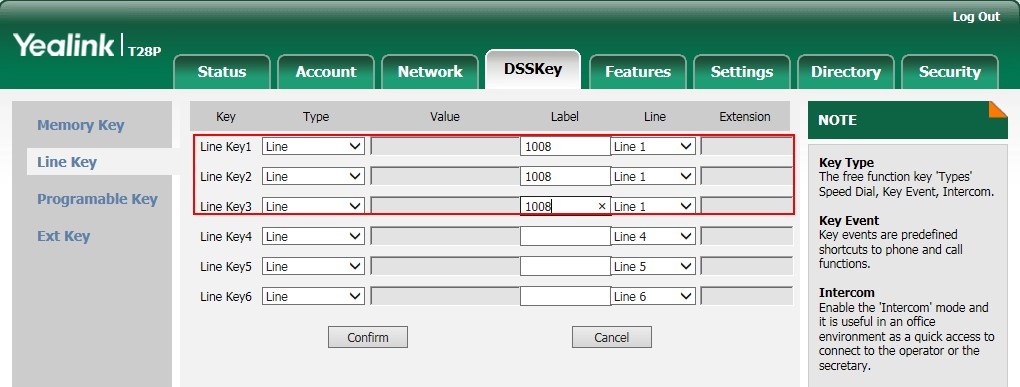
\includegraphics[width=0.29593in,height=0.21597in]{media/image471.png}
during an active call.

\begin{quote}
The LCD screen indicates that the call is now muted.

To un-mute a call:
\end{quote}

1. Press
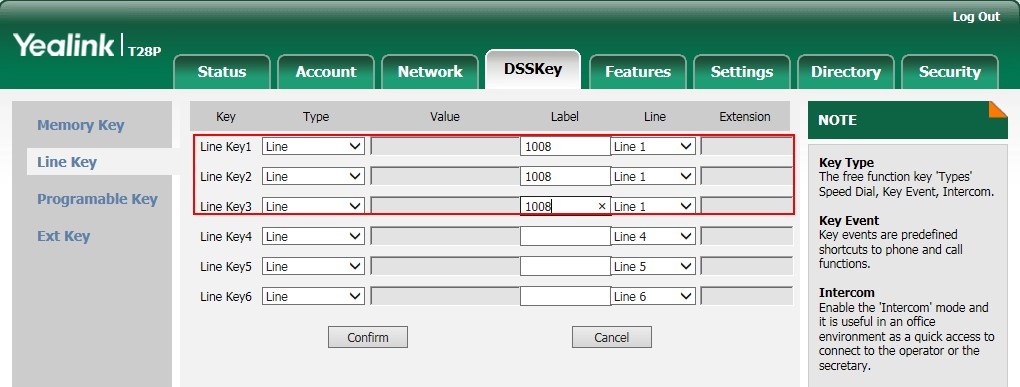
\includegraphics[width=0.29167in,height=0.21875in]{media/image471.png}
again to un-mute the call.


\includegraphics[width=1.92389in,height=0.28in]{media/image474.png}

\begin{quote}
You can place an active call on hold. Only one active call can be in
progress at any time. Other calls can be made and received while placing
the original call on hold. When you place a call on hold, your IP PBX
may play music to the other party while waiting.

To place a call on hold:
\end{quote}

1. Press

\includegraphics[width=0.29167in,height=0.21875in]{media/image431.png}
or the Hold soft key during a call.

The LCD screen indicates that the call is on hold and the line key LED
flashes green.

%\begin{longtable}[]{@{}
%>{\raggedright\arraybackslash}p{(\linewidth - 0\tabcolsep) * \real{1.0000}}@{}}
%\toprule\noalign{}
\begin{minipage}[b]{\linewidth}\raggedright
The phone will beep softly every 30 seconds to remind you that you still
have a call on hold.
\end{minipage} \\
%\midrule\noalign{}
%\endhead
%\bottomrule\noalign{}
%\endlastfoot
%\end{longtable}

Note

\begin{quote}
To resume a held call:
\end{quote}

1. Press

\includegraphics[width=0.29593in,height=0.21597in]{media/image431.png}
or the Resume soft key.

\begin{quote}
Multiple Calls on Hold:

If multiple calls are placed on hold, do one of the following:
\end{quote}

\begin{itemize}
\item
Press or to switch between the calls, and then press the Resume soft
key to retrieve the desired call.
\item
Press the corresponding line key to retrieve the desired call.
\end{itemize}

\begin{quote}
A numbered prompt appears on the LCD screen, for example "2/4",
indicating that this is the second call out of four calls.
\end{quote}


\includegraphics[width=2.29667in,height=0.28in]{media/image477.png}

\begin{quote}
You can use DND to reject incoming calls automatically on the phone. The
prompt message "n New Missed Call(s)" ("n" indicates the number of
missed calls) will appear on the LCD screen, and callers will receive a
busy message. All calls you receive while DND is enabled are logged to
your missed calls list.
\end{quote}

%\begin{longtable}[]{@{}
%>{\raggedright\arraybackslash}p{(\linewidth - 0\tabcolsep) * \real{1.0000}}@{}}
%\toprule\noalign{}
\begin{minipage}[b]{\linewidth}\raggedright
The prompt message will display only if Missed Call Log for the line is
enabled. Missed Call Log is configurable via web user interface at the
path Account-\textgreater Basic.

Do Not Disturb is local to the phone, and may be overridden by the
server settings. For more information, contact your system
administrator.
\end{minipage} \\
%\midrule\noalign{}
%\endhead
%\bottomrule\noalign{}
%\endlastfoot
%\end{longtable}

Note

\begin{quote}
You can enable/disable DND for the phone system, or you can customize
DND for each or all accounts. Two DND modes:
\end{quote}

\begin{itemize}
\item
Phone (default): DND is effective for the phone system.
\item
Custom: DND can be configured for each or all accounts.
\end{itemize}

\begin{quote}
You can receive incoming calls from authorized numbers when DND is
enabled.

To configure the DND mode via web user interface:
\end{quote}

\begin{enumerate}
\def\labelenumi{\arabic{enumi}.}
\item
Click on Features-\textgreater Forward \& DND.
\item
In the DND block, mark the desired radio box in the Mode field.
\item
Click Confirm to accept the change.
\end{enumerate}

Note DND mode is configurable via web user interface only.

\begin{quote}
To activate DND in phone mode:
\end{quote}

1. Press the DND soft key when the phone is idle.

\begin{quote}
The

\includegraphics[width=0.22917in,height=0.13541in]{media/image480.png}
icon on the idle screen indicates that DND is enabled.

Incoming calls will be rejected automatically and "n New Missed Call(s)"
("n" indicates the number of missed calls) will appear on the LCD
screen.
\end{quote}

%\begin{longtable}[]{@{}
%>{\raggedright\arraybackslash}p{(\linewidth - 0\tabcolsep) * \real{1.0000}}@{}}
%\toprule\noalign{}
\begin{minipage}[b]{\linewidth}\raggedright
When DND and busy forward are enabled in phone mode, calls will be sent
to the configured destination number. For more information on busy
forward, refer to Call Forward on page 88.
\end{minipage} \\
%\midrule\noalign{}
%\endhead
%\bottomrule\noalign{}
%\endlastfoot
%\end{longtable}

Note

\begin{quote}
To activate DND in custom mode for a specific account:
\end{quote}

1. Press the DND soft key when the phone is idle.

\begin{quote}
The LCD screen displays a list of the accounts on the phone.
\end{quote}

Press

or

to select the

desired account

and then press the

Enter

soft key.

Press

,

or the

Switch

soft key

to select

Enable

d

to

activate

DND

from the

\begin{quote}
2.

3.

DND Enable field.
\end{quote}

\begin{enumerate}
\def\labelenumi{\arabic{enumi}.}
\setcounter{enumi}{3}
\item
Press the Save soft key to accept the change.
\end{enumerate}

\begin{quote}
If you activate DND for the default account, the associated line icon
will change to

\includegraphics[width=0.12986in,height=0.13889in]{media/image486.png} ,
and the

\includegraphics[width=0.23333in,height=0.14097in]{media/image480.png}
icon will appear on the status bar.

If you activate DND for the non-default account, only the associated
line icon will change to

\includegraphics[width=0.12986in,height=0.13889in]{media/image486.png} .

Incoming calls on this line will be rejected automatically and "n New
Missed

Call(s)" ("n" indicates the number of missed calls) will prompt on the
LCD screen.
\end{quote}

%\begin{longtable}[]{@{}
%>{\raggedright\arraybackslash}p{(\linewidth - 0\tabcolsep) * \real{1.0000}}@{}}
%\toprule\noalign{}
\begin{minipage}[b]{\linewidth}\raggedright
When DND and busy forward are enabled for a specific account, calls from
the specific account will be sent to the configured destination number.
For more information on busy forward, refer to Call Forward on page 88.
\end{minipage} \\
%\midrule\noalign{}
%\endhead
%\bottomrule\noalign{}
%\endlastfoot
%\end{longtable}

Note

\begin{quote}
To activate DND in custom mode for all accounts:
\end{quote}

\begin{enumerate}
\def\labelenumi{\arabic{enumi}.}
\item
Press the DND soft key when the phone is idle.
\end{enumerate}

\begin{quote}
The LCD screen displays a list of the accounts on the phone.
\end{quote}

\begin{enumerate}
\def\labelenumi{\arabic{enumi}.}
\setcounter{enumi}{1}
\item
Press the All On soft key to activate DND for all accounts.
\item
Press the Save soft key to accept the change.
\end{enumerate}

\begin{quote}

\includegraphics[width=0.23333in,height=0.14097in]{media/image480.png}The
icon appears on the idle screen and all line icons change to

\includegraphics[width=0.13889in,height=0.13541in]{media/image486.png} .

Incoming calls will be rejected automatically and "n New Missed Call(s)"
("n" indicates the number of missed calls) will prompt on the LCD
screen.

To configure the DND authorized numbers via web user interface:
\end{quote}

\begin{enumerate}
\def\labelenumi{\arabic{enumi}.}
\item
Click on Features-\textgreater Forward \& DND.
\item
Select Enabled from the pull-down list of DND Emergency.
\item
Enter the numbers in the DND Authorized Numbers field.
\end{enumerate}

\begin{quote}
For multiple numbers, enter a comma between every two numbers.
\end{quote}

\begin{enumerate}
\def\labelenumi{\arabic{enumi}.}
\setcounter{enumi}{3}
\item
Click Confirm to accept the change.
\end{enumerate}

\begin{quote}
When DND is enabled on the phone, the phone can still receive incoming
calls from the numbers specified in the DND Authorized Numbers field.
\end{quote}

%\begin{longtable}[]{@{}
%>{\raggedright\arraybackslash}p{(\linewidth - 0\tabcolsep) * \real{1.0000}}@{}}
%\toprule\noalign{}
\begin{minipage}[b]{\linewidth}\raggedright
DND authorized number is configurable via web user interface only.

When the phone receives a voice mail, the voice mail prompt window will
pop up by default, if you want to disable the feature, contact your
system administrator for more information.
\end{minipage} \\
%\midrule\noalign{}
%\endhead
%\bottomrule\noalign{}
%\endlastfoot
%\end{longtable}

Note


\includegraphics[width=1.39431in,height=0.28in]{media/image494.png}

\begin{quote}
You can configure your phone to forward incoming calls to another party
through static forwarding. You can also forward calls while your phone
is ringing; refer to dynamic forwarding.
\end{quote}

%\subsection{\texorpdfstring{Static Forwarding
%}{Static Forwarding }}\label{static-forwarding}

\begin{quote}
Three types of static forwarding:
\end{quote}

\begin{itemize}
\item
Always Forward: Incoming calls are immediately forwarded.
\item
Busy Forward: Incoming calls are immediately forwarded if the phone is
busy.
\item
No Answer Forward: Incoming calls are forwarded if not answered after
a period
\end{itemize}

\begin{quote}
of time.

You can enable/disable call forward for the phone system, or you can
customize call forward for each or all accounts. Two call forward modes:
\end{quote}

\begin{itemize}
\item
Phone (default): Call forward is effective for the phone system.
\item
Custom: Call forward can be configured for each or all accounts.
\end{itemize}

\begin{quote}
To configure the call forward mode via web user interface:
\end{quote}

\begin{enumerate}
\def\labelenumi{\arabic{enumi}.}
\item
Click on Features-\textgreater Forward \& DND.
\item
In the Forward block, mark the desired radio box in the Mode field.
\end{enumerate}

3.

Click

Confirm

to accept the change.

Note Call forward mode is configurable via web user interface only.

\begin{quote}
To enable call forward in phone mode:
\end{quote}

\begin{enumerate}
\def\labelenumi{\arabic{enumi}.}
\item
Press Menu-\textgreater Features-\textgreater Call Forward.
\item
Press or to select the desired forwarding type, and then press the
Enter soft key.
\item
Depending on your selection:
\end{enumerate}

\begin{quote}
a.) If you select Always Forward:
\end{quote}

\begin{enumerate}
\def\labelenumi{\arabic{enumi})}
\item
Press or , or the Switch soft key to select Enabled from the Always
Forward field.
\item
Enter the destination number you want to forward incoming calls to in
the Forward to field.
\item
(Optional.) Enter the always forward on code and off code respectively
in the On Code and Off Code field.
\end{enumerate}

\begin{quote}
Always forward on code/ off code is used to activate/deactivate the
server-side always forward feature when the user enables/ disables
always forward feature on the phone.
\end{quote}

\begin{enumerate}
\def\labelenumi{\alph{enumi}.}
\setcounter{enumi}{1}
\item
If you select Busy Forward:

\begin{enumerate}
\def\labelenumii{\arabic{enumii})}
\item
Press or , or the Switch soft key to select Enabled from the Busy
Forward field.
\item
Enter the destination number you want to forward incoming calls to
when the phone is busy in the Forward to field.
\item
(Optional.) Enter the busy forward on code and off code respectively
in the On Code and Off Code field.
\end{enumerate}
\end{enumerate}

\begin{quote}
Busy forward on code/ off code is used to activate/deactivate the
server-side always forward feature when the user enables/ disables busy
forward feature on the phone.
\end{quote}

\begin{enumerate}
\def\labelenumi{\alph{enumi}.}
\setcounter{enumi}{2}
\item
If you select No Answer Forward:

\begin{enumerate}
\def\labelenumii{\arabic{enumii})}
\item
Press or , or the Switch soft key to select Enabled from the No
Answer Forward field.
\item
Enter the destination number you want to forward unanswered incoming
calls to in the Forward to field.
\item
Press or , or the Switch soft key to select the ring time to wait
before forwarding from the After Ring Time field.
\end{enumerate}
\end{enumerate}

\begin{quote}
The default ring time is 12 seconds.
\end{quote}

\begin{enumerate}
\def\labelenumi{\arabic{enumi})}
\setcounter{enumi}{3}
\item
(Optional.) Enter the no answer forward on code and off code
respectively in the On Code and Off Code field.
\end{enumerate}

\begin{quote}
No answer forward on code/ off code is used to activate/deactivate the

server-side always forward feature when the user enables/ disables no
answer forward feature on the phone.
\end{quote}

4. Press the Save soft key to accept the change.

\begin{quote}
The
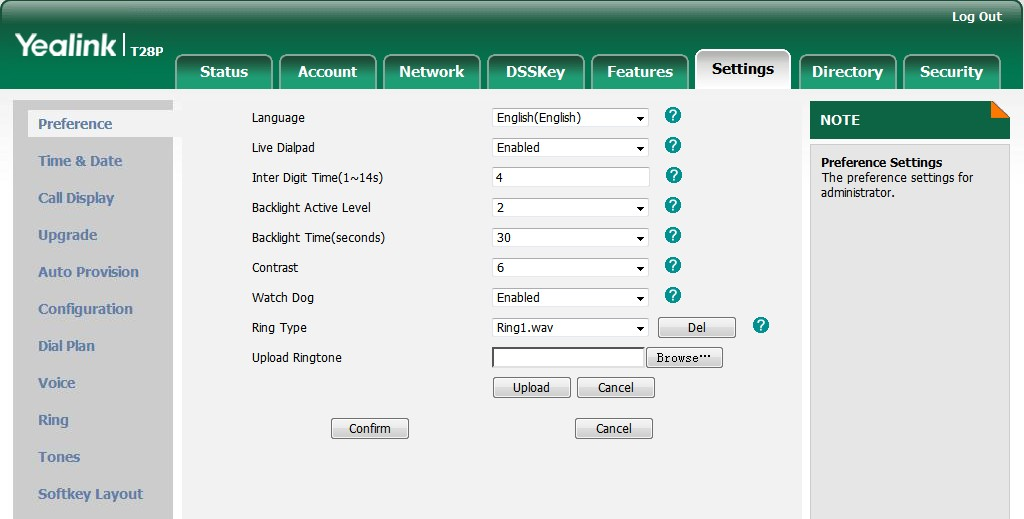
\includegraphics[width=0.12986in,height=0.13182in]{media/image503.png}
icon on the idle screen indicates that call forward is enabled.

To enable call forward in custom mode:
\end{quote}

\begin{enumerate}
\def\labelenumi{\arabic{enumi}.}
\item
Press Menu-\textgreater Features-\textgreater Call Forward.
\item
Press or to select the desired account, and then press the Enter soft
key.
\item
Press or to select the desired forwarding type, and then press the
Enter soft key.
\item
Depending on your selection:
\end{enumerate}

\begin{quote}
a.) If you select Always Forward, you can enable it for a specific
account.
\end{quote}

\begin{enumerate}
\def\labelenumi{\arabic{enumi})}
\item
Press or , or the Switch soft key to select Enabled from the Always
Forward field.
\item
Enter the destination number you want to forward incoming calls to in
the Forward to field.
\item
(Optional.) Enter the always forward on code and off code respectively
in the On Code and Off Code field.
\end{enumerate}

\begin{quote}
Always forward on code/ off code is used to activate/deactivate the
server-side always forward feature when the user enables/ disables
always forward feature for this account.

You can also enable always forward for all accounts. After always
forward was enabled for a specific account, do the following:
\end{quote}

\begin{enumerate}
\def\labelenumi{\arabic{enumi})}
\item
Press or to select the Always Forward field.
\item
Press the All Lines soft key.
\end{enumerate}

\begin{quote}
The LCD screen prompts ``Copy to all lines?''.
\end{quote}

\begin{enumerate}
\def\labelenumi{\arabic{enumi})}
\setcounter{enumi}{2}
\item
Press the OK soft key to accept the change or the Cancel soft key to
cancel.
\end{enumerate}

\begin{enumerate}
\def\labelenumi{\alph{enumi}.}
\setcounter{enumi}{1}
\item
If you select Busy Forward, you can enable it for a specific account.

\begin{enumerate}
\def\labelenumii{\arabic{enumii})}
\item
Press or , or the Switch soft key to select Enabled from the Busy
Forward field.
\item
Enter the destination number you want to forward incoming calls to
when the phone is busy in the Forward to field.
\item
(Optional.) Enter the busy forward on code and off code respectively
in the On Code and Off Code field.
\end{enumerate}
\end{enumerate}

\begin{quote}
Busy forward on code/ off code is used to activate/deactivate the
server-side always forward feature when the user enables/ disables busy
forward feature for this account.

You can also enable busy forward for all accounts. After busy forward
was enabled for a specific account, do the following:
\end{quote}

\begin{enumerate}
\def\labelenumi{\arabic{enumi})}
\item
Press or to select the Busy Forward field.
\item
Press the All Lines soft key.
\end{enumerate}

\begin{quote}
The LCD screen prompts ``Copy to all lines?''.
\end{quote}

\begin{enumerate}
\def\labelenumi{\arabic{enumi})}
\setcounter{enumi}{2}
\item
Press the OK soft key to accept the change or the Cancel soft key to
cancel.
\end{enumerate}

\begin{enumerate}
\def\labelenumi{\alph{enumi}.}
\setcounter{enumi}{2}
\item
If you select No Answer Forward, you can enable it for a specific
account.

\begin{enumerate}
\def\labelenumii{\arabic{enumii})}
\item
Press or , or the Switch soft key to select Enabled from the No
Answer Forward field.
\item
Enter the destination number you want to forward unanswered incoming
calls to in the Forward to field.
\item
Press or , or the Switch soft key to select the ring time to wait
before forwarding from the After Ring Time field.
\end{enumerate}
\end{enumerate}

\begin{quote}
The default ring time is 12 seconds.
\end{quote}

\begin{enumerate}
\def\labelenumi{\arabic{enumi})}
\setcounter{enumi}{3}
\item
(Optional.) Enter the no answer forward on code and off code
respectively in the On Code and Off Code field.
\end{enumerate}

\begin{quote}
No answer forward on code/ off code is used to activate/deactivate the
server-side always forward feature when the user enables/ disables no
answer forward feature for this account.

You can also enable no answer forward for all accounts. After no answer
forward was enabled for a specific account, do the following:
\end{quote}

\begin{enumerate}
\def\labelenumi{\arabic{enumi})}
\item
Press or to select the No Answer Forward field.
\item
Press the All Lines soft key.
\end{enumerate}

The LCD screen prompts

``

Copy to all l

ines?

''

.

\begin{enumerate}
\def\labelenumi{\arabic{enumi})}
\setcounter{enumi}{2}
\item
Press the OK soft key to accept the change or the Cancel soft key to
cancel.
\end{enumerate}

5. Press the Save soft key to accept the change or the Back soft key to
cancel.

\begin{quote}
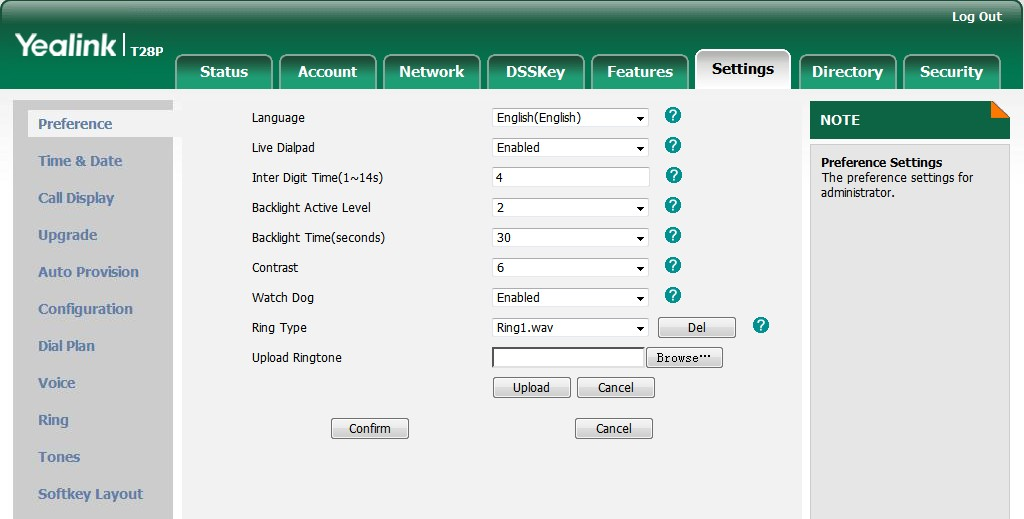
\includegraphics[width=0.12986in,height=0.13194in]{media/image503.png}If
you activate call forward for the default account, the associated line
icon will change to , and the

\includegraphics[width=0.13055in,height=0.12778in]{media/image516.png}
icon will appear on the status bar.

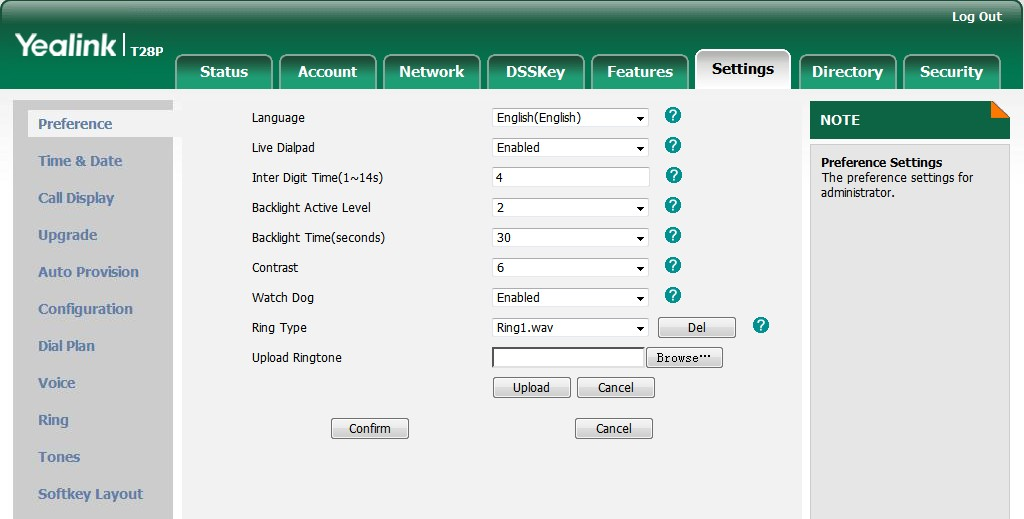
\includegraphics[width=0.12986in,height=0.13194in]{media/image503.png}If
you activate call forward for the non-default account, only the
associated line icon will change to .

Call forward is configurable via web user interface at the path
Features-\textgreater Forward \& DND.
\end{quote}

%\begin{longtable}[]{@{}
%>{\raggedright\arraybackslash}p{(\linewidth - 0\tabcolsep) * \real{1.0000}}@{}}
%\toprule\noalign{}
\begin{minipage}[b]{\linewidth}\raggedright
You can also enter the SIP URI or IP address in the Forward to field.
For more information on using the SIP URI or IP address, refer to
Placing Calls on page 73.

Call forward is local to the phone, and may be overridden by the server
settings. Call forward on code or off code may be different between
servers. For more information, contact your system administrator.
\end{minipage} \\
%\midrule\noalign{}
%\endhead
%\bottomrule\noalign{}
%\endlastfoot
%\end{longtable}

Note

\begin{quote}
To disable call forward in phone mode:

Do one of the following:
\end{quote}

\begin{itemize}
\item
Press

\includegraphics[width=0.29097in,height=0.21586in]{media/image517.png}
when the phone is idle.
\item
Press Menu-\textgreater Features-\textgreater Call Forward.
\end{itemize}

\begin{quote}
Press or to select the desired forwarding type, then press the Enter
soft key.
\end{quote}

Press or , or the Switch soft key to select Disabled to disable call
forward.

\begin{quote}
Press the Save soft key to accept the change.

To disable call forward in custom mode for a specific account:
\end{quote}

\begin{enumerate}
\def\labelenumi{\arabic{enumi}.}
\item
Press Menu-\textgreater Features-\textgreater Call Forward or press

\includegraphics[width=0.28958in,height=0.21699in]{media/image517.png}
when the phone is idle.
\item
Press or to select the desired account and then press the Enter soft
key.
\item
Press or to select the desired forwarding type, then press the Enter
soft key.
\item
Press , or the Switch soft key to select Disabled to disable call
forward.
\item
Press the Save soft key to accept the change.
\end{enumerate}

%\subsection{\texorpdfstring{Dynamic Forwarding
%}{Dynamic Forwarding }}\label{dynamic-forwarding}

\begin{quote}
To forward an incoming call to another party:
\end{quote}

\begin{enumerate}
\def\labelenumi{\arabic{enumi}.}
\item
When the phone is ringing, press the Forward soft key.
\item
Enter the number you want to forward the incoming call to.
\end{enumerate}

3.

Press

,

,

or the

Send

soft key.

\begin{quote}
The LCD screen prompts a call forward message.
\end{quote}

%\begin{longtable}[]{@{}
%>{\raggedright\arraybackslash}p{(\linewidth - 0\tabcolsep) * \real{1.0000}}@{}}
%\toprule\noalign{}
\begin{minipage}[b]{\linewidth}\raggedright
When the phone forwards a call, the forward call prompt window will pop
up by default, if you want to disable the feature, contact your system
administrator for more information.
\end{minipage} \\
%\midrule\noalign{}
%\endhead
%\bottomrule\noalign{}
%\endlastfoot
%\end{longtable}

Note

\begin{quote}
You can transfer a call to another party in one of three ways:
\end{quote}

\begin{itemize}
\item
Blind Transfer: Transfer a call directly to another party without
consulting.
\item
Semi-Attended Transfer: Transfer a call when the target phone is
ringing.
\item
Attended Transfer: Transfer a call with prior consulting.
\end{itemize}

\begin{quote}
To perform a blind transfer:
\end{quote}

\begin{enumerate}
\def\labelenumi{\arabic{enumi}.}
\item
Press

\includegraphics[width=0.29167in,height=0.21699in]{media/image517.png}
or the Transfer soft key during a call.
\item
Do one of the following:
\end{enumerate}

- Enter the number or you want to transfer the call to.

\begin{enumerate}
\def\labelenumi{\arabic{enumi}.}
\setcounter{enumi}{2}
\item
Press

\includegraphics[width=0.29167in,height=0.21699in]{media/image517.png}
to complete the transfer.
\end{enumerate}

\begin{quote}
Then the call is connected to the number to which you are transferring.

To perform a semi-attended transfer:
\end{quote}

\begin{enumerate}
\def\labelenumi{\arabic{enumi}.}
\item
Press

\includegraphics[width=0.29593in,height=0.21597in]{media/image517.png}
or the Transfer soft key during a call.
\item
Do one of the following:
\end{enumerate}

\begin{itemize}
\item
Enter the number you want to transfer the call to.
\item
Press the Directory soft key, and then select Local Directory. Select
the desired group, and search for the contact (Directory should be
configured in advance. Refer to Local Directory on page 33 for more
information.).
\item
Press the Directory soft key, and then select History. Select the
desired list and use or to select the entry (Directory should be
configured in advance.
\end{itemize}

\begin{quote}
Refer to Local Directory on page 33 for more information.).
\end{quote}

\begin{itemize}
\item
Press the Directory soft key, and then select Remote Phone Book.
Select the desired group and search for the contact (Directory and
remote phone book should be configured in advance. Refer to Local
Directory on page 33 and Remote Phone Book on page 46 for more
information.)
\end{itemize}

\begin{enumerate}
\def\labelenumi{\arabic{enumi}.}
\setcounter{enumi}{2}
\item
Press or to dial out.
\item
Press or the Transfer soft key to complete the transfer when receiving
ringback.
\end{enumerate}

\begin{quote}
To perform an attended transfer:
\end{quote}

\begin{enumerate}
\def\labelenumi{\arabic{enumi}.}
\item
Press

\includegraphics[width=0.29167in,height=0.21528in]{media/image517.png}
or the Transfer soft key during a call.
\item
Do one of the following:

\begin{itemize}
\item
Enter the number you want to transfer the call to.
\item
Press the Directory soft key, and then select Local Directory.
Select the desired group, and search for the contact (Directory
should be configured in advance. Refer to Local Directory on page 33
for more information.).
\item
Press the Directory soft key, and then select History. Select the
desired list and use or to select the entry (Directory should be
configured in advance.
\end{itemize}
\end{enumerate}

\begin{quote}
Refer to Local Directory on page 33 for more information.).
\end{quote}

\begin{itemize}
\item
Press the Directory soft key, and then select Remote Phone Book.
Select the desired group and search for the contact (Directory and
remote phone book should be configured in advance. Refer to Local
Directory on page 33 and Remote Phone Book on page 46 for more
information.)
\end{itemize}

\begin{enumerate}
\def\labelenumi{\arabic{enumi}.}
\setcounter{enumi}{2}
\item
Press the Send soft key, or to dial out.
\item
After the party answers the call, press or the Transfer soft key to
complete the transfer.
\end{enumerate}

\begin{quote}
If you are using a handset, the transfer can be completed by hanging up
the handset.

You can cancel the transfer before the call is connected by pressing the
Cancel soft key.
\end{quote}


\includegraphics[width=1.33647in,height=0.28in]{media/image523.png}

\begin{quote}
You can enable or disable call waiting on the phone. If call waiting is
enabled, you can receive another call while there is already an active
call on the phone. Otherwise, another incoming call is automatically
rejected by the phone with a busy message when there is an active call
on the phone. You can also enable or disable the phone to play a warning
tone when receiving another call.

To configure call waiting via phone user interface:
\end{quote}

\begin{enumerate}
\def\labelenumi{\arabic{enumi}.}
\item
Press Menu-\textgreater Features-\textgreater Call Waiting.
\item
Press or , or the Switch soft key to select Enabled from the Call
Waiting field.
\item
Press or , or the Switch soft key to select Enabled from the Play Tone
field.
\item
(Optional.) Enter the call waiting on code and off code respectively
in the On Code and Off Code field.
\end{enumerate}

\begin{quote}
Call waiting on code/ off code is used to activate/deactivate the
server-side call waiting feature when the user enables/ disables call
waiting feature on the phone.
\end{quote}

\begin{enumerate}
\def\labelenumi{\arabic{enumi}.}
\setcounter{enumi}{4}
\item
Press the Save soft key to accept the change or the Back soft key to
cancel.
\end{enumerate}

\begin{quote}
Call waiting is configurable via web user interface at the path
Features-\textgreater General Information.
\end{quote}


\includegraphics[width=1.28736in,height=0.28in]{media/image526.png}

\begin{quote}
You can create a conference with other two parties using the phone's
local conference. You can create a conference between an active call and
a call on hold (on the same or another line) by pressing the CONF key or
the Conf soft key.
\end{quote}

%\begin{longtable}[]{@{}
%>{\raggedright\arraybackslash}p{(\linewidth - 0\tabcolsep) * \real{1.0000}}@{}}
%\toprule\noalign{}
\begin{minipage}[b]{\linewidth}\raggedright
Network conference is not available on all servers. For more
information, contact your system administrator.
\end{minipage} \\
%\midrule\noalign{}
%\endhead
%\bottomrule\noalign{}
%\endlastfoot
%\end{longtable}

Note


\includegraphics[width=1.63347in,height=0.24333in]{media/image527.png}

\begin{quote}
The SIP-T28P IP phone supports up to 3 parties (including yourself) in a
conference call.

This is the default method of conference called Local Conference.

To set up a local conference call:
\end{quote}

\begin{enumerate}
\def\labelenumi{\arabic{enumi}.}
\item
Place a call to the first party.
\item
When the first party answers the call, press

\includegraphics[width=0.29167in,height=0.21699in]{media/image528.png}
or the Conf soft key to place a new call.
\end{enumerate}

\begin{quote}
The active call is placed on hold.
\end{quote}

3.

Enter the number

of

the

second party

and press

,

,

or the

Send

soft key.

\begin{enumerate}
\def\labelenumi{\arabic{enumi}.}
\setcounter{enumi}{3}
\item
When the second party answers the call, you can consult with him or
her before adding to the conference.
\item
Press

\includegraphics[width=0.29167in,height=0.21699in]{media/image528.png}
or the Conf soft key again to join all parties in the conference.
\end{enumerate}

\begin{quote}
To join two calls in a conference:
\end{quote}

\begin{enumerate}
\def\labelenumi{\arabic{enumi}.}
\item
Place two calls using two different accounts on the phone (for
example, place the first call using account 1, and then place the
second call using account 2).
\item
Press or to select the call for conference and ensure that the call is
active (for example, select the call on account 1).
\item
Press

\includegraphics[width=0.29167in,height=0.21699in]{media/image528.png}
or the Conf soft key to join the two calls in the conference on the
selected account.
\end{enumerate}

\begin{quote}
You can press

\includegraphics[width=0.29593in,height=0.21597in]{media/image431.png}
or the Hold soft key to place the conference on hold. You can press the
Split soft key to split the conference call into two individual calls on
hold. To drop the conference call, press the Cancel soft key.
\end{quote}


\includegraphics[width=1.94292in,height=0.24333in]{media/image533.png}

\begin{quote}
You can use network conference on the SIP-T28P IP phone to conduct a
conference with multiple participants.

This feature allows you to perform the following:
\end{quote}

\begin{itemize}
\item
Join two calls together into a conference call.
\item
Invite another party into an active conference call.
\end{itemize}

\begin{quote}
To use this feature, contact your system administrator for the network
conference URI in advance.

To configure network conference via web user interface:
\end{quote}

\begin{enumerate}
\def\labelenumi{\arabic{enumi}.}
\item
Click on Account.
\item
Select the desired account from the pull-down list of Account.
\item
Click on Advanced.
\item
Select Network Conference from the pull-down list of Conference Type.
\item
Enter the conference URI (e.g., conference@example.com) in the
Conference URI field.
\end{enumerate}

6.

Click

Confirm

to accept the

change

.

%\begin{longtable}[]{@{}
%>{\raggedright\arraybackslash}p{(\linewidth - 0\tabcolsep) * \real{1.0000}}@{}}
%\toprule\noalign{}
\begin{minipage}[b]{\linewidth}\raggedright
Network conference is configurable via web user interface only.
\end{minipage} \\
%\midrule\noalign{}
%\endhead
%\bottomrule\noalign{}
%\endlastfoot
%\end{longtable}

Note

\begin{quote}
To set up a network conference call:
\end{quote}

\begin{enumerate}
\def\labelenumi{\arabic{enumi}.}
\item
Place a call to the first party.
\item
Press

\includegraphics[width=0.29593in,height=0.21597in]{media/image528.png}
or the Conf soft key to place a new call.
\end{enumerate}

\begin{quote}
The active call is placed on hold.
\end{quote}

\begin{enumerate}
\def\labelenumi{\arabic{enumi}.}
\setcounter{enumi}{2}
\item
Enter the number of the second party and press , , or the Send soft
key.
\item
When the second party answers the call, press or the Conf soft key to
add the second party to the conference.
\item
Press

\includegraphics[width=0.29167in,height=0.21699in]{media/image528.png}
or the Conf soft key to place a new call.
\end{enumerate}

\begin{quote}
The conference is placed on hold.
\end{quote}

\begin{enumerate}
\def\labelenumi{\arabic{enumi}.}
\setcounter{enumi}{5}
\item
Enter the number of the new party and then press , , or the Send soft
key.
\item
When the new party answers the call, press or the Conf soft key to add
the new party to the conference.
\item
Repeat steps 5 to 7 until you have added all intended parties.
\end{enumerate}

\begin{quote}
The procedures to set up a network conference call for specific servers
may be different from introduced above. Contact your system
administrator for more information.
\end{quote}


\includegraphics[width=0.98926in,height=0.28in]{media/image537.png}

\begin{quote}
You can use call park to place a call on hold, and then retrieve the
call from another phone in the system (for example, a phone in another
office or conference room). You can park an active call by pressing the
call park key on the phone. If the call is parked successfully, the
response is either a voice prompt confirming that the call was parked,
or a visible prompt on the LCD screen.
\end{quote}

%\begin{longtable}[]{@{}
%>{\raggedright\arraybackslash}p{(\linewidth - 0\tabcolsep) * \real{1.0000}}@{}}
%\toprule\noalign{}
\begin{minipage}[b]{\linewidth}\raggedright
Call park is not available on all servers. Contact your system
administrator for more information.
\end{minipage} \\
%\midrule\noalign{}
%\endhead
%\bottomrule\noalign{}
%\endlastfoot
%\end{longtable}

Note

\begin{quote}
To configure a call park key via phone user interface:
\end{quote}

\begin{enumerate}
\def\labelenumi{\arabic{enumi}.}
\item
Press Menu-\textgreater Features-\textgreater DSS
Keys-\textgreater Memory Keys (or Line Keys).
\item
Select the desired DSS key.
\item
Press or , or the Switch soft key to select Key Event from the Type
field.
\item
Press or , or the Switch soft key to select Call Park from the Key
Type field.
\item
Press or , or the Switch soft key to select the desired account from
the Account ID field.
\item
Enter the call park code in the Value field.
\item
Press the Save soft key to accept the change or the Back soft key to
cancel.
\end{enumerate}

\begin{quote}
Call park key is configurable via web user interface at the path DSSKey.

To use call park:
\end{quote}

\begin{enumerate}
\def\labelenumi{\arabic{enumi}.}
\item
User on phone A places a call to phone B.
\item
User on phone A wants to take the call in a conference room for
privacy, and so presses the call park key on phone A.
\item
User on phone A walks to an available conference room where the phone
is designated as phone C. The user dials call park retrieve code to
retrieve the parked call.
\end{enumerate}

\begin{quote}
The system establishes call between phone C and B.
\end{quote}

%\begin{longtable}[]{@{}
%>{\raggedright\arraybackslash}p{(\linewidth - 0\tabcolsep) * \real{1.0000}}@{}}
%\toprule\noalign{}
\begin{minipage}[b]{\linewidth}\raggedright
The call park code and call park retrieve code are predefined on the
system server. Contact your system administrator for more information.

If the parked call is not retrieved within a period of time assigned by
the system, the phone performing call park will receive a call back.
\end{minipage} \\
%\midrule\noalign{}
%\endhead
%\bottomrule\noalign{}
%\endlastfoot
%\end{longtable}

Note

\begin{quote}
You can use call pickup to answer someone else's incoming call on your
phone. The SIP-T28P IP phone supports directed call pickup and group
call pickup. Directed call pickup is used for picking up a call that is
ringing at a target phone number. Group call pickup is used for picking
up a call that is ringing at any phone number in a certain group. The
pickup group should be predefined, contact your system administrator for
more information.

You can pick up an incoming call by using the DPickup/GPickup soft key.
To use call pickup, you need to configure the call pickup code
beforehand on a global or per-line basis via web user interface.

Note If there are many incoming calls at the same time, pressing the
GPickup soft key on the phone will pick up the call that rings first.

The directed call pickup code and group call pickup code are predefined
on the system server. Contact your system administrator for more
information.

The call pickup code configured on a per-line basis takes precedence
over that configured on a global basis.
\end{quote}

%\section{\texorpdfstring{Directed Call Pickup
%}{Directed Call Pickup }}\label{directed-call-pickup}

\begin{quote}
To enable the directed call pickup via web user interface:
\end{quote}

\begin{enumerate}
\def\labelenumi{\arabic{enumi}.}
\item
Click on Features-\textgreater Call Pickup.
\item
Select Enabled from the pull-down list of Directed Call Pickup.
\item
Click Confirm to accept the change.
\end{enumerate}

\begin{quote}
To configure the directed call pickup code on a global basis via web
user interface:
\end{quote}

\begin{enumerate}
\def\labelenumi{\arabic{enumi}.}
\item
Click on Features-\textgreater Call Pickup.
\item
Enter the directed call pickup code in the Directed Call Pickup Code
field.
\item
Click Confirm to accept the change.
\end{enumerate}

\begin{quote}
To configure the directed call pickup code on a per-line basis via web
user interface:
\end{quote}

\begin{enumerate}
\def\labelenumi{\arabic{enumi}.}
\item
Click on Account.
\item
Select the desired account from the pull-down list of Account.
\item
Click on Advanced.
\item
Enter the directed call pickup code in the Directed Call Pickup Code
field.
\item
Click Confirm to accept the change.
\end{enumerate}

\begin{quote}
To pick up a call directly:
\end{quote}

\begin{enumerate}
\def\labelenumi{\arabic{enumi}.}
\item
Pick up the handset and press the more soft key.
\end{enumerate}

\begin{quote}
The DPickup soft key appears on the LCD screen.
\end{quote}

\begin{enumerate}
\def\labelenumi{\arabic{enumi}.}
\setcounter{enumi}{1}
\item
Press the DPickup soft key on your phone when the target phone
receives an incoming call.
\item
Enter the phone number which is receiving an incoming call.
\item
Press the DPickup soft key again.
\end{enumerate}

\begin{quote}
The call is answered on your phone.

You can also configure a DSS key as a directed pickup key via phone user
interface or web user interface. Once configured, you can pick up a call
by pressing the directed pickup key directly.
\end{quote}

Note If a pickup code is already configured on a global or a per -line
basis, you should not configure the pickup code when configuring a DSS
key to be pickup key.

%\section{\texorpdfstring{Group Call Pickup
%}{Group Call Pickup }}\label{group-call-pickup}

\begin{quote}
To enable group call pickup via web user interface:
\end{quote}

\begin{enumerate}
\def\labelenumi{\arabic{enumi}.}
\item
Click on Features-\textgreater Call Pickup.
\item
Select Enabled from the pull-down list of Group Call Pickup.
\item
Click Confirm to accept the change.
\end{enumerate}

\begin{quote}
To configure the group call pickup code on a global basis via web user
interface:
\end{quote}

\begin{enumerate}
\def\labelenumi{\arabic{enumi}.}
\item
Click on Features-\textgreater Call Pickup.
\item
Enter the group call pickup code in the Group Call Pickup Code field.
\item
Click Confirm to accept the change.
\end{enumerate}

\begin{quote}
To configure the group call pickup code on a per-line basis via web user
interface:
\end{quote}

\begin{enumerate}
\def\labelenumi{\arabic{enumi}.}
\item
Click on Account.
\item
Select the desired account from the pull-down list of Account.
\item
Click on Advanced.
\item
Enter the group call pickup code in the Group Call Pickup Code field.
\item
Click Confirm to accept the change.
\end{enumerate}

\begin{quote}
To pick up a call in the group:
\end{quote}

\begin{enumerate}
\def\labelenumi{\arabic{enumi}.}
\item
Pick up the handset.
\end{enumerate}

\begin{quote}
The GPickup soft key appears on the LCD screen.
\end{quote}

\begin{enumerate}
\def\labelenumi{\arabic{enumi}.}
\setcounter{enumi}{1}
\item
Press the GPickup soft key on your phone when a phone in the group
receives an incoming call.
\end{enumerate}

\begin{quote}
The call is answered on your phone.

You can also configure a DSS key as a group pickup key via phone user
interface or web user interface. Once configured, you can pick up a call
by pressing the group pickup key directly.
\end{quote}

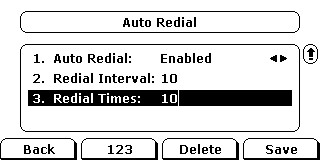
\includegraphics[width=1.77931in,height=0.28in]{media/image556.png}

\begin{quote}
You can use anonymous call to block your identify and phone number from
appearing to the called party when you call someone. For example, you
want to call to consult some of the services, but don't want to be
harassed. Anonymous call is configurable on a per-line basis. You can
also configure the phone to send anonymous call on/off code to the
server to activate/deactivate anonymous call on the server side.
\end{quote}

%\begin{longtable}[]{@{}
%>{\raggedright\arraybackslash}p{(\linewidth - 0\tabcolsep) * \real{1.0000}}@{}}
%\toprule\noalign{}
\begin{minipage}[b]{\linewidth}\raggedright
Anonymous call is not available on all servers. Contact your system
administrator for the anonymous call on code and off code.
\end{minipage} \\
%\midrule\noalign{}
%\endhead
%\bottomrule\noalign{}
%\endlastfoot
%\end{longtable}

Note

\begin{quote}
To configure anonymous call via phone user interface:
\end{quote}

1. Press Menu-\textgreater Features-\textgreater Anonymous Call.

\begin{quote}
2.

ID field.
\end{quote}

Press

or

,

or the

Switch

soft key

to select the desired line

from the

Account

Press

or

to select

Enable

d

from the

Local

Anonymous

field.

(

Optional.

)

Press or

to select

the desired value

from the

Send Anony Code

\begin{quote}
3.

4.

field.
\end{quote}

\begin{enumerate}
\def\labelenumi{\arabic{enumi}.}
\setcounter{enumi}{4}
\item
(Optional.) Enter the anonymous call on code and off code respectively
in the On Code and Off Code field.
\end{enumerate}

\begin{quote}
The phone will send the configured on code or off code depending on your
selection when you enable or disable anonymous call feature on the
phone.
\end{quote}

\begin{enumerate}
\def\labelenumi{\arabic{enumi}.}
\setcounter{enumi}{5}
\item
Press the Save soft key to accept the change or the Back soft key to
cancel.
\end{enumerate}

\begin{quote}
Anonymous call is configurable via web user interface at the path
Account-\textgreater Basic.

To place an anonymous call:
\end{quote}

1. Using the specific line on the phone to place a call to phone B.

\begin{quote}
The LCD screen of phone B prompts an incoming call from anonymity.
\end{quote}

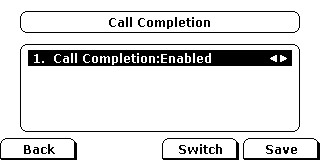
\includegraphics[width=2.78583in,height=0.28in]{media/image561.png}

\begin{quote}
You can use anonymous call rejection to reject incoming calls from
anonymous callers. Anonymous call rejection automatically rejects
incoming calls from callers who deliberately block their identities and
numbers from being displayed. Anonymous call rejection is configurable
on a per-line basis. You can also configure the phone to send anonymous
call rejection on/off code to the server to activate/deactivate
anonymous call rejection on the server side.

To configure anonymous call rejection via phone user interface:
\end{quote}

1. Press Menu-\textgreater Features-\textgreater Anonymous Call.

\begin{quote}
2.

ID field.
\end{quote}

Press

or

, or the

Switch

soft key to

select the desired line

from

the

Account

Press

or

to scroll to the

Anon

Reject

field.

Press

or

to select

Enable

d

from

the

Anon

Reject

field.

Press or to scroll to the

Send

r

ejection Code

field.

(

Optional.) Press or

to select

the desired value

from the

Send

r

ejection

\begin{quote}
3.

4.

5.

6.

Code field.
\end{quote}

\begin{enumerate}
\def\labelenumi{\arabic{enumi}.}
\setcounter{enumi}{6}
\item
(Optional.) Enter the anonymous call rejection on code and off code
respectively in the On Code and Off Code field.
\end{enumerate}

\begin{quote}
The phone will send the configured on code or off code depending on your
selection when you enable or disable local anonymous rejection feature
on the phone.
\end{quote}

\begin{enumerate}
\def\labelenumi{\arabic{enumi}.}
\setcounter{enumi}{7}
\item
Press the Save soft key to accept the change or the Back soft key to
cancel.
\end{enumerate}

\begin{quote}
Anonymous call rejection is configurable via web user interface at the
path Account-\textgreater Basic.

This chapter provides operating instructions for the advanced features
of the SIP-T28P IP phone. Topics include:
\end{quote}

\begin{itemize}
\item
Busy Lamp Field (BLF)
\item
BLF List
\item
Call Recording
\item
Hot Desking
\item
Intercom
\item
Multicast Paging
\item
Music on Hold
\item
Messages
\end{itemize}

\begin{quote}
If you require additional information or assistance with your new phone,
contact your system administrator.

You can use BLF to monitor a specific line for status changes on the
phone. For example, you can configure a BLF key on the phone to monitor
the status of a friend's line (busy or idle). The BLF key LED slow
flashing green when the friend\textquotesingle s line is in use. For
more information on BLF key LED indications, refer to LED Instructions
on page 4.

You can press a BLF key to dial out the monitored phone number when the
monitored line is idle. You can receive a visual or/and an audio alert
(if enabled), and also pick up calls that are received on the monitored
line. For more information, contact your system administrator.

To configure a BLF key via phone user interface:
\end{quote}

\begin{enumerate}
\def\labelenumi{\arabic{enumi}.}
\item
Press Menu-\textgreater Features-\textgreater DSS
Keys-\textgreater Memory Keys (or Line Keys).
\item
Select the desired DSS key.
\item
Press or , or the Switch soft key to select BLF from the Type field.
\item
Press or , or the Switch soft key to select the desired account from
the Account ID field.
\item
Enter the phone number or extension you want to monitor in the Value
field.
\item
(Optional.) Enter the pickup code in the Extension field.
\item
Press the Save soft key to accept the change or the Back soft key to
cancel.
\end{enumerate}

\begin{quote}
BLF key is configurable via web user interface at the path DSSKey.

You can enable audio alert feature for BLF pickup on the phone. This
allows the phone to play a warning tone when the monitored line receives
an incoming call. You can also enable visual alert feature for BLF
pickup on the phone. This allows the LCD screen of the monitoring phone
to display the caller ID when the monitored line receives an incoming
call.

To enable visual and audio alert features via web user interface:
\end{quote}

\begin{enumerate}
\def\labelenumi{\arabic{enumi}.}
\item
Click on Features-\textgreater Call Pickup.
\item
Select Enabled from the pull-down list of Visual Alert for BLF Pickup.
3. Select Enabled from the pull-down list of Audio Alert for BLF
Pickup.
\end{enumerate}

4.

Click

Confirm

to

accept the change

.

%\begin{longtable}[]{@{}
%>{\raggedright\arraybackslash}p{(\linewidth - 0\tabcolsep) * \real{1.0000}}@{}}
%\toprule\noalign{}
\begin{minipage}[b]{\linewidth}\raggedright
Visual and audio alert features are configurable via web user interface
only.
\end{minipage} \\
%\midrule\noalign{}
%\endhead
%\bottomrule\noalign{}
%\endlastfoot
%\end{longtable}

Note

\begin{quote}
When the monitored line receives an incoming call, the following occurs
on your phone:
\end{quote}

\begin{itemize}
\item
The phone plays a warning tone (if enabled).
\item
The BLF key LED flashes.
\item
The caller ID appears on the LCD screen (if enabled).
\end{itemize}

\begin{quote}
In the following figure, the LCD screen shows an incoming call from 2388
on the monitored line.
\end{quote}

%\begin{longtable}[]{@{}
%>{\raggedright\arraybackslash}p{(\linewidth - 0\tabcolsep) * \real{1.0000}}@{}}
%\toprule\noalign{}
\begin{minipage}[b]{\linewidth}\raggedright
If your phone is locked and the type of the phone lock is configured as
Function Keys or

All Keys, you cannot use the Pickup, Send, New Call and Cancel soft keys
until unlocked.
\end{minipage} \\
%\midrule\noalign{}
%\endhead
%\bottomrule\noalign{}
%\endlastfoot
%\end{longtable}

Note

\begin{quote}
When there is an active call on the IP phone, you can transfer the
active call to the monitored phone number directly by pressing the BLF
key. The phone handles the active call differently depending on the
transfer mode on DSS key. For more information on the transfer mode on
DSS key, refer to transfer in DSS Keys section on page 53.

You can use the BLF List feature to monitor a list of users defined by
your system administrator. For example, your system administrator
enables BLF List, and creates a BLF List URI (e.g., BLFList@example.com)
including a list of user1, user2 on the server. The BLF List keys on the
IP phone can present the status of user1 and user2. The key LEDs
illuminate either flashing or solid depending on the status of those
users. For more BLF List key LED indications, refer to LED Instructions
on page 4.

You can use the BLF List keys in the following ways:
\end{quote}

\begin{itemize}
\item
When the monitored user is idle, press the BLF list key to dial out
the phone number.
\item
When there is already an active call on the IP phone, you can transfer
the active call to the monitored user by pressing the BLF List key.
The phone handles the active call differently depending on the
transfer mode on DSS key. For more information on the transfer mode on
DSS key, refer to Transfer section on page 58.
\item
When the monitored user receives an incoming call, press the BLF list
key to pick up the call directly. Before picking up an incoming call,
ensure that the directed pickup code has been configured in advance.
If the directed pickup code is not configured, the phone will place a
call to the monitored user instead of picking up the incoming call of
the monitored user when you press the BLF List key.
\item
When there is a conversation on the monitored user, press the BLF list
key to barge in and set up a conference call. Before barging in an
active call, ensure that the barge-in code has been configured in
advance. If the BLF list barge in code is not configured, the phone
will place a call to the monitored user instead of barging in an
active call of the monitored user when you press the BLF List key.
\item
When a call is being parked against the monitored phone, press the BLF
List key to retrieve the parked call from the monitored user. Before
retrieving the parked call, ensure that the BLF List Retrieve call
parked Code has been configured in advance. If the code is not
configured, the phone will place a call to the monitored user instead
of retrieving the parked call when you press the BLF List key.
\end{itemize}

\begin{quote}
To configure BLF List settings via web user interface:
\end{quote}

\begin{enumerate}
\def\labelenumi{\arabic{enumi}.}
\item
Click on Account-\textgreater Advanced.
\item
Select the desired account from the pull-down list of Account.
\item
Enter the BLF List URI in the BLF List URI field.
\item
(Optional.) Enter the directed pickup code in the BLF List code field.
\item
(Optional.) Enter the barge-in code in the BLF List Barge In Code
field.
\item
(Optional.) Enter the call park retrieve code in the BLF List Retrieve
call parked Code field.
\item
Click Confirm to accept the change.
\end{enumerate}

%\begin{longtable}[]{@{}
%>{\raggedright\arraybackslash}p{(\linewidth - 0\tabcolsep) * \real{1.0000}}@{}}
%\toprule\noalign{}
\begin{minipage}[b]{\linewidth}\raggedright
For more information on BLF List URI/BLF List Code/BLF List Barge In
Code/BLF List Retrieve Call Parked Code, contact your system
administrator.
\end{minipage} \\
%\midrule\noalign{}
%\endhead
%\bottomrule\noalign{}
%\endlastfoot
%\end{longtable}

Note

\begin{quote}
According to the response message from the server, the IP phone will
automatically configure the BLF List keys beginning from the first
unused DSS key (The default order of BLF list keys assigned
automatically is Line Key-\textgreater Memory Key-\textgreater Ext Key).
Once any DSS key is seized, the IP phone will skip to configure the next
DSS key.

You can receive a visual or/and an audio alert (if enabled) on your
phone when the monitored user receives an incoming call. For more
information, refer to Busy Lamp Field (BLF) on page 109.
\end{quote}

%\begin{longtable}[]{@{}
%>{\raggedright\arraybackslash}p{(\linewidth - 0\tabcolsep) * \real{1.0000}}@{}}
%\toprule\noalign{}
\begin{minipage}[b]{\linewidth}\raggedright
The pickup code is used in the following order of preference: BLF List
Code

(Account-\textgreater Advanced)\textgreater Directed Call Pickup Code
(Account-\textgreater Advanced)\textgreater Directed Call Pickup Code
(Features-\textgreater Call Pickup). If all of them are not configured,
pressing the BLF List key will directly call the monitored user when
he/she receives an incoming call.

For more information about pickup Code, refer to Call Pickup on page
101.
\end{minipage} \\
%\midrule\noalign{}
%\endhead
%\bottomrule\noalign{}
%\endlastfoot
%\end{longtable}

Note


\includegraphics[width=1.58292in,height=0.28in]{media/image584.png}

\begin{quote}
You can record calls by pressing a record key on the phone. The SIP-T28P
IP phone supports record and URL record.

Two ways of call recording:
\end{quote}

\begin{itemize}
\item
Record: The phone sends SIP INFO message containing a specific header
``Record: on/off'' to trigger a recording.
\item
URL Record: The phone sends HTTP URL request to trigger a recording.
Contact your system administrator for the predefined URL.
\end{itemize}

Note Call record is not available on all servers. Contact your system
administrator for more information.

\begin{quote}
To configure a record key via phone user interface:
\end{quote}

\begin{enumerate}
\def\labelenumi{\arabic{enumi}.}
\item
Press Menu-\textgreater Features-\textgreater DSS Keys-\textgreater(or
Line Keys).
\item
Select the desired DSS key.
\end{enumerate}

3.

Press

or

, or the

Switch

soft key

to select

Key Event

from the

Type

field.

4.

Press

or

, or the

Switch

soft key

to select

Record

from the

Key Type

field.

5. Press the Save soft key to accept the change or the Back soft key to
cancel.

\begin{quote}
To configure a URL record key via phone user interface:
\end{quote}

\begin{enumerate}
\def\labelenumi{\arabic{enumi}.}
\item
Press Menu-\textgreater Features-\textgreater DSS
Keys-\textgreater Memory Keys (or Line Keys).
\item
Select the desired DSS key.
\item
Press or , or the Switch soft key to select URL Record from the Type
field.
\item
Enter the URL (e.g., http://10.1.2.224/phonerecording.cgi) in the
Value field.
\item
Press the Save soft key to accept the change or the Back soft key to
cancel.
\end{enumerate}

\begin{quote}
Record and URL record keys are configurable via web user interface at
the path DSSKey.

The record and URL record keys control the recording function, and are
available:
\end{quote}

\begin{itemize}
\item
During an active call
\item
When calls are on hold or muted
\item
During a blind or attended transfer
\item
During a conference call
\item
When the phone prompts you to answer an incoming call The record and
URL record keys are not available when:
\item
There are no connected calls on your phone
\item
You place a new call To record a call:
\end{itemize}

\begin{enumerate}
\def\labelenumi{\arabic{enumi}.}
\item
Press a record or URL record key during a call.
\end{enumerate}

\begin{quote}
If the recording starts successfully, the recording icon will appear on
the LCD screen and the record or URL record key LED will flash green.
\end{quote}

\begin{enumerate}
\def\labelenumi{\arabic{enumi}.}
\setcounter{enumi}{1}
\item
Press the record or URL record key again to stop recording.
\end{enumerate}

\begin{quote}
The recording icon disappears from the LCD screen and the record or URL
record key LED goes out.

Recording status indications you need to know:
\end{quote}

%\begin{longtable}[]{@{}
%>{\raggedright\arraybackslash}p{(\linewidth - 2\tabcolsep) * \real{0.4312}}
%>{\raggedright\arraybackslash}p{(\linewidth - 2\tabcolsep) * \real{0.5688}}@{}}
%\toprule\noalign{}
\begin{minipage}[b]{\linewidth}\centering
Circumstance
%\end{minipage} & \begin{minipage}[b]{\linewidth}\centering
Icons on the LCD screen
\end{minipage} \\
%\midrule\noalign{}
%\endhead
%\bottomrule\noalign{}
%\endlastfoot
%A recording is started & \begin{minipage}[t]{\linewidth}\raggedright
\begin{quote}

\includegraphics[width=0.14167in,height=0.13889in]{media/image589.png}
appears on the LCD screen
\end{quote}
%\end{minipage} \\
%A recording cannot be started &
\begin{minipage}[t]{\linewidth}\raggedright
\begin{quote}

\includegraphics[width=0.16042in,height=0.15972in]{media/image590.png}
appears for 1 second
\end{quote}
\end{minipage} \\
%A recording cannot be stopped &
\begin{minipage}[t]{\linewidth}\raggedright
\begin{quote}

\includegraphics[width=0.15278in,height=0.18056in]{media/image591.png}
appears for 1 second, then goes back
\end{quote}
\end{minipage} \\
%The recording box is full & \begin{minipage}[t]{\linewidth}\raggedright
\begin{quote}

\includegraphics[width=0.17917in,height=0.18056in]{media/image592.png}
appears for 1 second
\end{quote}
%\end{minipage} \\
%The call cannot be recorded &
\begin{minipage}[t]{\linewidth}\raggedright
\begin{quote}
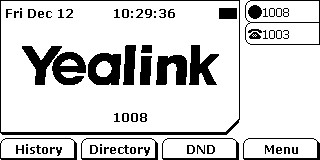
\includegraphics[width=0.16042in,height=0.18056in]{media/image593.png}
appears for 1 second
\end{quote}
\end{minipage} \\
%\end{longtable}

\begin{quote}
You can listen to the recordings stored on your server system. For
example, you can dial an access code to listen to the recordings.
\end{quote}

%\begin{longtable}[]{@{}
%>{\raggedright\arraybackslash}p{(\linewidth - 0\tabcolsep) * \real{1.0000}}@{}}
%\toprule\noalign{}
\begin{minipage}[b]{\linewidth}\raggedright
The way in which you listen to the recordings may be different depending
on the server. Contact your system administrator for more information.
\end{minipage} \\
%\midrule\noalign{}
%\endhead
%\bottomrule\noalign{}
%\endlastfoot
%\end{longtable}

Note


\includegraphics[width=1.36764in,height=0.28in]{media/image594.png}

\begin{quote}
Hot desking originates from the definition of being the temporary
physical occupant of a work station or surface by a particular employee.
A primary motivation for hot desking is cost reduction. This feature is
regularly used in places where not all the employees are in the office
at the same time, or not in the office for very long, which means that
actual personal offices would be often vacant, consuming valuable space
and resources.

You can use hot desking on the SIP-T28P IP phone to log out of existing
accounts and then log into a new account, that is, many users can share
the phone resource at different times. To use this feature, you need to
configure a hot desking key in advance.
\end{quote}

%\begin{longtable}[]{@{}
%>{\raggedright\arraybackslash}p{(\linewidth - 0\tabcolsep) * \real{1.0000}}@{}}
%\toprule\noalign{}
\begin{minipage}[b]{\linewidth}\raggedright
Hot desking is not available on all servers. Contact your system
administrator for more information.
\end{minipage} \\
%\midrule\noalign{}
%\endhead
%\bottomrule\noalign{}
%\endlastfoot
%\end{longtable}

Note

\begin{quote}
To configure a hot desking key via phone user interface:
\end{quote}

\begin{enumerate}
\def\labelenumi{\arabic{enumi}.}
\item
Press Menu-\textgreater Features-\textgreater DSS
Keys-\textgreater Memory Keys (or Line Keys).
\item
Select the desired DSS key.
\item
Press or , or the Switch soft key to select Key Event from the Type
field.
\end{enumerate}

\begin{quote}
field.
\end{quote}

4.

Press

or

, or the

Switch

soft key

to select

Hot Desking

from the

Key Type

5. Press the Save soft key to accept the change or the Back soft key to
cancel.

\begin{quote}
Hot desking key is configurable via web user interface at the path
DSSKey.

To use hot desking:
\end{quote}

\begin{enumerate}
\def\labelenumi{\arabic{enumi}.}
\item
Press the hot desking key when the phone is idle.
\end{enumerate}

\begin{quote}
The LCD screen prompts ``Clear all account config?''.
\end{quote}

\begin{enumerate}
\def\labelenumi{\arabic{enumi}.}
\setcounter{enumi}{1}
\item
Press the OK soft key, registration configurations of all accounts
will be cleared immediately.
\end{enumerate}

\begin{quote}
The login wizard will be displayed as below:
\end{quote}

\begin{enumerate}
\def\labelenumi{\arabic{enumi}.}
\setcounter{enumi}{2}
\item
Enter the desired values in the User Name and Password fields
respectively.
\end{enumerate}

\begin{quote}
Contact your system administrator for more information.
\end{quote}

\begin{enumerate}
\def\labelenumi{\arabic{enumi}.}
\setcounter{enumi}{3}
\item
Press the Save soft key to login or Cancel soft key to cancel.
\end{enumerate}


\includegraphics[width=1.04663in,height=0.28in]{media/image601.png}

\begin{quote}
Intercom is a useful feature in an office environment to quickly connect
with the operator or the secretary. You can press the intercom key to
automatically connect with a remote extension for outgoing intercom
calls, and the remote extension will automatically answer incoming
intercom calls.
\end{quote}

%\begin{longtable}[]{@{}
%>{\raggedright\arraybackslash}p{(\linewidth - 0\tabcolsep) * \real{1.0000}}@{}}
%\toprule\noalign{}
\begin{minipage}[b]{\linewidth}\raggedright
Intercom is not available on all servers. Contact your system
administrator for more information.
\end{minipage} \\
%\midrule\noalign{}
%\endhead
%\bottomrule\noalign{}
%\endlastfoot
%\end{longtable}

Note

\begin{quote}
To configure an intercom key via phone user interface:
\end{quote}

\begin{enumerate}
\def\labelenumi{\arabic{enumi}.}
\item
Press Menu-\textgreater Features-\textgreater DSS
Keys-\textgreater Memory Keys (or Line Keys).
\item
Select the desired DSS key.
\item
Press or , or the Switch soft key to select Intercom from the Type
field.
\item
Select the desired account from the Account ID field.
\item
Enter the remote extension number in the Value field.
\item
Press the Save soft key to accept the change or the Back soft key to
cancel.
\end{enumerate}

\begin{quote}
Intercom key is configurable via web user interface at the path DSSKey.

To place an intercom call:
\end{quote}

\begin{enumerate}
\def\labelenumi{\arabic{enumi}.}
\item
Press the intercom key when the phone is idle.
\end{enumerate}

The phone is automatically connected to the extension specified in the
Value field.

\begin{enumerate}
\def\labelenumi{\arabic{enumi}.}
\setcounter{enumi}{1}
\item
Press the intercom key again or the Cancel soft key to end the
intercom call.
\end{enumerate}

\begin{quote}
The SIP-T28P IP phone supports automatically to answer an incoming
intercom call by default. The phone automatically plays a warning tone
when it receives an incoming intercom call. In addition, you can enable
the phone to mute the microphone when it automatically answers an
incoming intercom call. You can also enable the phone to automatically
answer an incoming intercom call while there is already an active call
on the phone. The active call is then placed on hold.

Intercom features you need to know:
\end{quote}

%\begin{longtable}[]{@{}
%>{\raggedright\arraybackslash}p{(\linewidth - 2\tabcolsep) * \real{0.2697}}
%>{\raggedright\arraybackslash}p{(\linewidth - 2\tabcolsep) * \real{0.7303}}@{}}
%\toprule\noalign{}
\begin{minipage}[b]{\linewidth}\raggedright
\begin{quote}
Intercom Feature
\end{quote}
%\end{minipage} & \begin{minipage}[b]{\linewidth}\centering
\begin{quote}
Description
\end{quote}
\end{minipage} \\
%\midrule\noalign{}
%\endhead
%\bottomrule\noalign{}
%\endlastfoot
%Accept Intercom & \begin{minipage}[t]{\linewidth}\raggedright
\begin{quote}
Enable or disable the IP phone to automatically answer an incoming
intercom call.
\end{quote}
%\end{minipage} \\
%Intercom Mute & \begin{minipage}[t]{\linewidth}\raggedright
\begin{quote}
Enable or disable the IP phone's microphone for intercom calls.
\end{quote}
%\end{minipage} \\
%Intercom Tone & \begin{minipage}[t]{\linewidth}\raggedright
\begin{quote}
Enable or disable the IP phone to play a warning tone when it receives
an incoming intercom call.
\end{quote}
%\end{minipage} \\
%Intercom Barge & \begin{minipage}[t]{\linewidth}\raggedright
\begin{quote}
Enable or disable the IP phone to automatically answer an incoming
intercom call while there is already an active call on the phone.
\end{quote}
%\end{minipage} \\
%\end{longtable}

\begin{quote}
To configure intercom features via phone user interface:
\end{quote}

\begin{enumerate}
\def\labelenumi{\arabic{enumi}.}
\item
Press Menu-\textgreater Features-\textgreater Intercom.
\item
Make the desired changes.
\item
Press the Save soft key to accept the change or the Back soft key to
cancel.
\end{enumerate}

\begin{quote}
These specific parameters are configurable via web user interface at the
path Features-\textgreater Intercom.

Accept Intercom

You can enable or disable the phone to automatically answer an incoming
intercom call. If Accept Intercom is enabled, the phone will
automatically answer an incoming intercom call. If Accept Intercom is
disabled, the phone will reject incoming intercom calls and send a busy
message to the caller. Accept Intercom is enabled by default.
\end{quote}

%\begin{longtable}[]{@{}
%>{\raggedright\arraybackslash}p{(\linewidth - 0\tabcolsep) * \real{1.0000}}@{}}
%\toprule\noalign{}
\begin{minipage}[b]{\linewidth}\raggedright
Your administrator can set a delay time before the phone automatically
answers intercom calls. Contact your system administrator for more
information.
\end{minipage} \\
%\midrule\noalign{}
%\endhead
%\bottomrule\noalign{}
%\endlastfoot
%\end{longtable}

Note

\begin{quote}
Intercom Mute

You can mute or un-mute the phone's microphone for intercom calls
automatically. If

Intercom Mute is enabled, the microphone will be muted for intercom
calls. If Intercom Mute is disabled, the microphone will work for
intercom calls. Intercom Mute is disabled by default.

Intercom Tone

You can enable or disable the phone to play a warning tone when
receiving an intercom call. If Intercom Tone is enabled, the phone will
play a warning tone before answering the intercom call. If Intercom Tone
is disabled, the phone will automatically answer the intercom call
without warning. Intercom Tone is enabled by default.

Intercom Barge

You can enable or disable the phone to automatically answer an incoming
intercom call while there is already an active call on the phone. If
Intercom Barge is enabled, the phone will automatically answer the
intercom call and place the active call on hold. If Intercom Barge is
disabled, the phone will handle an incoming intercom call like a waiting
call. Intercom Barge is disabled by default.
\end{quote}


\includegraphics[width=1.82819in,height=0.28in]{media/image624.png}

\begin{quote}
You can use multicast paging to quickly and easily forward out time
sensitive announcements to people within the multicast group. You can
configure a multicast paging key or a paging list key on the phone,
which allows you to send a Real Time Transport Protocol (RTP) stream to
the pre-configured multicast address(es) without involving SIP
signaling. You can configure the phone to receive an RTP stream from
pre-configured multicast listening address(es) without involving SIP
signaling. You can specify up to 10 multicast listening addresses.

To configure a multicast paging key via phone user interface:
\end{quote}

\begin{enumerate}
\def\labelenumi{\arabic{enumi}.}
\item
Press Menu-\textgreater Features-\textgreater DSS
Keys-\textgreater Memory Keys (or Line Keys).
\item
Select the desired DSS key.
\item
Press or , or the Switch soft key to select Key Event from the Type
field.
\item
Press or , or the Switch soft key to select Multicast Paging from the
Key Type field.
\item
Enter the multicast IP address and port number (e.g.,
224.5.6.20:10008) in the Value field.
\end{enumerate}

\begin{quote}
The valid multicast IP addresses range from 224.0.0.0 to
239.255.255.255.
\end{quote}

\begin{enumerate}
\def\labelenumi{\arabic{enumi}.}
\setcounter{enumi}{5}
\item
Press the Save soft key to accept the change or the Back soft key to
cancel.
\end{enumerate}

\begin{quote}
Multicast paging key is configurable via web user interface at the path
DSSKey.

To configure a paging list key via phone user interface:
\end{quote}

\begin{enumerate}
\def\labelenumi{\arabic{enumi}.}
\item
Press Menu-\textgreater Features-\textgreater DSS
Keys-\textgreater Memory Keys (or Line Keys).
\item
Select the desired DSS key.
\end{enumerate}

\begin{quote}
3.

4.

field.
\end{quote}

Press

or

, or the Switch soft key

to select

Key Event

from the

Type

field.

Press

or

, or the Switch soft key

to select

Paging

List

from the

Key Type

5. Press the Save soft key to accept the change or the Back soft key to
cancel.

\begin{quote}
Paging list key is configurable via web user interface at the path
DSSKey.

To configure paging list via phone user interface:
\end{quote}

\begin{enumerate}
\def\labelenumi{\arabic{enumi}.}
\item
Press the paging list key when the phone is idle.
\item
Press or to select a desired paging group.
\end{enumerate}

\begin{quote}
The default tag is Empty if it is not configured before.
\end{quote}

\begin{enumerate}
\def\labelenumi{\arabic{enumi}.}
\setcounter{enumi}{2}
\item
Press the Option soft key.
\item
Press the Edit soft key.
\item
Enter the multicast IP address and port number (e.g.,
224.5.6.20:10008) in the Address field.
\end{enumerate}

\begin{quote}
The valid multicast IP addresses range from 224.0.0.0 to
239.255.255.255.
\end{quote}

\begin{enumerate}
\def\labelenumi{\arabic{enumi}.}
\setcounter{enumi}{5}
\item
Enter the group name in the Label field.
\item
Press the Save soft key to accept the change.
\item
Repeat the step 2-7, you can add more paging groups.
\end{enumerate}

\begin{quote}
Paging list is configurable via web user interface at the path:
Directory-\textgreater Multicast IP.

To delete paging group via phone user interface:
\end{quote}

\begin{enumerate}
\def\labelenumi{\arabic{enumi}.}
\item
Press the Paging list key when the phone is idle.
\item
Press or to select a desired group.
\item
Press the Option soft key.
\item
Press the Delete soft key.
\item
Press the OK soft key to accept the change or the Cancel soft key to
cancel.
\end{enumerate}

\begin{quote}
If you want to delete all paging group, you can press the Delete All
soft key.

You can also configure the phone to use a default codec for sending
multicast RTP stream via web user interface.

To configure a default codec for multicast paging via web user
interface:
\end{quote}

\begin{enumerate}
\def\labelenumi{\arabic{enumi}.}
\item
Click on Features-\textgreater General Information.
\item
Select the desired codec from the pull-down list of Multicast Codec.
\end{enumerate}

\begin{quote}
The default codec is G722.
\end{quote}

3.

Click

Confirm

to accept the change.

%\begin{longtable}[]{@{}
%>{\raggedright\arraybackslash}p{(\linewidth - 0\tabcolsep) * \real{1.0000}}@{}}
%\toprule\noalign{}
\begin{minipage}[b]{\linewidth}\raggedright
If G722 codec is used for multicast paging, the LCD screen will display
the

\includegraphics[width=0.19375in,height=0.15278in]{media/image641.png}
icon to indicate that it is providing high definition voice.

Default codec for multicast paging is configurable via web user
interface only.
\end{minipage} \\
%\midrule\noalign{}
%\endhead
%\bottomrule\noalign{}
%\endlastfoot
%\end{longtable}

Note

\begin{quote}
To send RTP stream via a multicast paging key:
\end{quote}

\begin{enumerate}
\def\labelenumi{\arabic{enumi}.}
\item
Press the multicast paging key when the phone is idle.
\end{enumerate}

\begin{quote}
The phone sends RTP to a preconfigured multicast address (IP: Port). Any
phone in the local network then listens to the RTP on the preconfigured
multicast address (IP: Port). For both sending and receiving of the
multicast RTP, there is no SIP signaling involved.

The multicast paging key LED illuminates solid green.

The following figure shows a multicast RTP session on the phone:
\end{quote}

\begin{enumerate}
\def\labelenumi{\arabic{enumi}.}
\setcounter{enumi}{1}
\item
Press the Hold soft key to place the current multicast RTP session on
hold.
\item
Press the Cancel soft key to cancel the multicast RTP session.
\end{enumerate}

%\begin{longtable}[]{@{}
%>{\raggedright\arraybackslash}p{(\linewidth - 0\tabcolsep) * \real{1.0000}}@{}}
%\toprule\noalign{}
\begin{minipage}[b]{\linewidth}\raggedright
Multicast RTP is one way only from the sender to the multicast
address(es) (receiver). For outgoing RTP multicasts, all other existing
calls on the phone will be placed on hold.
\end{minipage} \\
%\midrule\noalign{}
%\endhead
%\bottomrule\noalign{}
%\endlastfoot
%\end{longtable}

Note

\begin{quote}
To send RTP stream via a paging key list:
\end{quote}

1. Press the paging list key when the phone is idle.

\begin{quote}
2.
\end{quote}

Press

or

to select the

desired group

.

Press

or

the

Paging

soft key

to

send

RT

P

.

\begin{quote}
3.
\end{quote}

\begin{enumerate}
\def\labelenumi{\arabic{enumi}.}
\setcounter{enumi}{3}
\item
Press the Hold soft key to place the current multicast RTP session on
hold.
\item
Press the Cancel soft key to cancel the multicast RTP session.
\end{enumerate}

\begin{quote}
You can configure the phone to receive a Real Time Transport Protocol
(RTP) stream from the pre-configured multicast address(es) without
involving SIP signaling. You can specify up to 10 multicast addresses
that the phone listens to on the network.

How the phone handles incoming multicast paging calls depends on Paging
Barge and Paging Priority Active parameters configured via web user
interface.

Paging Barge

The paging barge parameter defines the priority of the voice call in
progress. If the priority of an incoming multicast paging call is lower
than that of the active call, it will be ignored automatically. If
Disabled is selected from the pull-down list of Paging Barge, the voice
call in progress will take precedence over all incoming multicast paging
calls.

Valid values in the Paging Barge field:
\end{quote}

\begin{itemize}
\item
1 to 10: Define the priority of the active call, 1 is the highest
priority, 10 is the lowest.
\item
Disabled: The voice call in progress will take precedence over all
incoming paging calls.
\end{itemize}

\begin{quote}
Paging Priority Active

The paging priority active parameter decides how the phone handles
incoming multicast paging calls when there is already a multicast paging
call on the phone. If enabled, the phone will ignore incoming multicast
paging calls with lower priorities, otherwise, the phone will answer
incoming multicast paging calls automatically and place the previous
multicast paging call on hold. If disabled, the phone will automatically
ignore all incoming multicast paging calls.

To configure multicast listening addresses via web user interface:
\end{quote}

\begin{enumerate}
\def\labelenumi{\arabic{enumi}.}
\item
Select the desired value from the pull-down list of Paging Barge.
\item
Select the desired value from the pull-down list of Paging Priority
Active.
\item
Enter the multicast IP address(es) and port number (e.g.,
224.5.6.20:10008) which the phone listens to for incoming RTP
multicast in the Listening Address field.
\end{enumerate}

\begin{quote}
The valid multicast IP addresses range from 224.0.0.0 to
239.255.255.255.
\end{quote}

\begin{enumerate}
\def\labelenumi{\arabic{enumi}.}
\setcounter{enumi}{5}
\item
Enter the label in the Label field.
\end{enumerate}

\begin{quote}
Label will appear on the LCD screen when receiving the RTP multicast.
\end{quote}

\begin{enumerate}
\def\labelenumi{\arabic{enumi}.}
\setcounter{enumi}{6}
\item
Click Confirm to accept the change.
\end{enumerate}

%\begin{longtable}[]{@{}
%>{\raggedright\arraybackslash}p{(\linewidth - 0\tabcolsep) * \real{1.0000}}@{}}
%\toprule\noalign{}
\begin{minipage}[b]{\linewidth}\raggedright
The priorities of listening addresses are predefined: 1 with the highest
priority, 10 with the lowest.

Both the multicast paging sender and receiver's phones play a warning
tone when establishing a multicast paging call.

Multicast listening addresses are configurable via web user interface
only.
\end{minipage} \\
%\midrule\noalign{}
%\endhead
%\bottomrule\noalign{}
%\endlastfoot
%\end{longtable}

Note


\includegraphics[width=1.55514in,height=0.28in]{media/image650.png}

\begin{quote}
Music on hold (MoH) is the business practice of playing recorded music
to fill the silence that would be heard by the party placed on hold. To
use this feature, you should specify a SIP URI pointing to a Music on
Hold Server account. When a call is placed on hold, the phone will send
a SIP INVITE message to the Music on Hold Server account. The Music on
Hold Server account automatically answers the SIP INVITE messages and
immediately plays audio from some source located anywhere (LAN,
Internet) to the held party. Contact your system administrator for the
SIP URI. To configure the music on hold server via web user interface:
\end{quote}

\begin{enumerate}
\def\labelenumi{\arabic{enumi}.}
\item
Click on Account.
\item
Select the desired account from the pull-down list of Account.
\item
Click on Advanced.
\item
Enter the SIP URI (e.g., sip:moh@sip.com) in the Music Server URI
field.
\item
Click Confirm to accept the change.
\end{enumerate}

\begin{quote}
When you have placed a call on hold, the held party can hear the music.
\end{quote}

%\begin{longtable}[]{@{}
%>{\raggedright\arraybackslash}p{(\linewidth - 0\tabcolsep) * \real{1.0000}}@{}}
%\toprule\noalign{}
\begin{minipage}[b]{\linewidth}\raggedright
For this feature to function, all involved parties cannot use encrypted
RTP (SRTP).

Music on hold server is configurable via the web user interface only.
\end{minipage} \\
%\midrule\noalign{}
%\endhead
%\bottomrule\noalign{}
%\endlastfoot
%\end{longtable}

Note

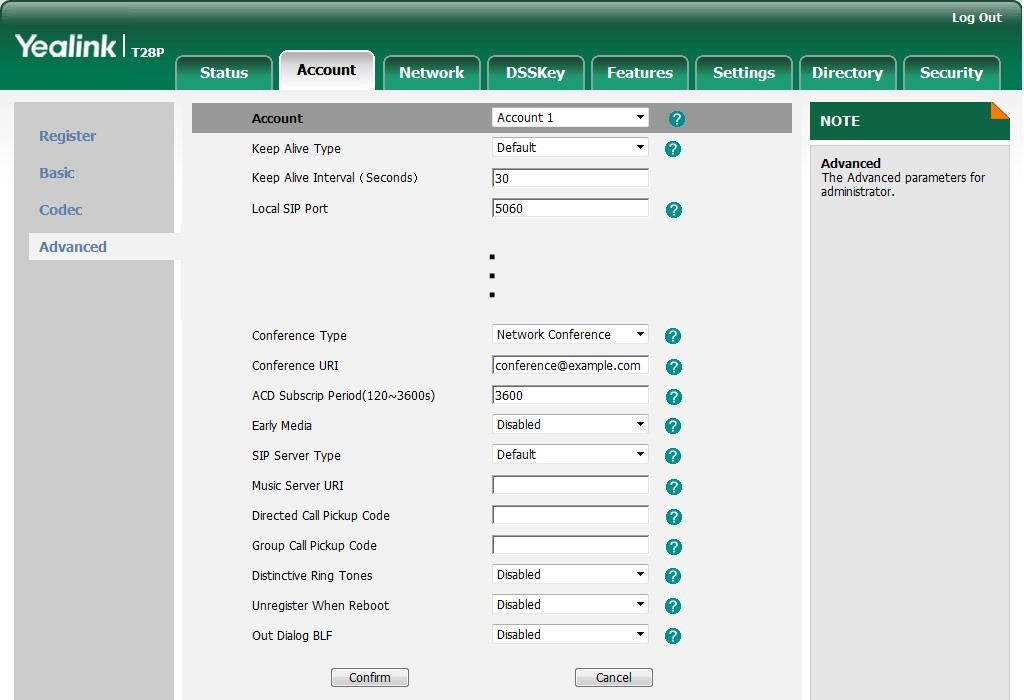
\includegraphics[width=1.11413in,height=0.28in]{media/image653.png}

\begin{quote}
You can send and receive text messages using the SIP-T28P IP phone. New
text messages can be indicated both acoustically and visually. When
receiving a new text message, the phone will play a warning tone, and
the LCD screen will prompt receiving new text messages with the number
of waiting messages (example: 2 New Text Message(s)) and a flashing
icon.
\end{quote}

Note When the phone receives a text message, the text message prompt
window will pop up by default, if you want to disable the feature,
contact your system administrator for more information.

\begin{quote}
You can store text messages in your phone's Inbox, Sentbox, Outbox or
Draftbox. Each of the boxes can store up to 100 text messages. If the
number of the text messages in one box is more than 100, the phone will
directly delete the oldest text message in the box.
\end{quote}

Note SMS is not available on all servers. Contact your system
administrator for more information.

\begin{quote}
To read a text message:
\end{quote}

\begin{enumerate}
\def\labelenumi{\arabic{enumi}.}
\item
Press Menu-\textgreater Messages-\textgreater Text
Message-\textgreater Inbox.
\item
Select the desired message and press the View soft key.
\end{enumerate}

%\begin{longtable}[]{@{}
%>{\raggedright\arraybackslash}p{(\linewidth - 0\tabcolsep) * \real{1.0000}}@{}}
%\toprule\noalign{}
\begin{minipage}[b]{\linewidth}\raggedright
If the phone prompts receiving new text messages, you can also press the
View soft key to read the new messages directly.
\end{minipage} \\
%\midrule\noalign{}
%\endhead
%\bottomrule\noalign{}
%\endlastfoot
%\end{longtable}

Note

\begin{quote}
To send a text message:
\end{quote}

\begin{enumerate}
\def\labelenumi{\arabic{enumi}.}
\item
Press Menu-\textgreater Messages-\textgreater Text
Message-\textgreater New Message.
\item
Compose the new text message. You can press the abc soft key to change
the input mode.
\item
Press the Send soft key.
\item
(Optional.) Press or , or the Switch soft key to select the desired
account from the From field.
\item
Enter the number you want to send the message to in the To field.
\item
Press the Send soft key to send the message or the Back soft key to
cancel.
\end{enumerate}

\begin{quote}
Sending a text message is configurable via web user interface at the
path Features-\textgreater SMS.

To reply a text message:
\end{quote}

\begin{enumerate}
\def\labelenumi{\arabic{enumi}.}
\item
Press Menu-\textgreater Messages-\textgreater Text
Message-\textgreater Inbox.
\item
Select the desired message and press the Reply soft key.
\item
Compose the new text message. You can press the abc soft key to change
the input mode.
\item
Press the Send soft key after completing the content.
\item
Check the From and To fields, and then press the Send soft key.
\end{enumerate}

\begin{quote}
To delete a text message:
\end{quote}

\begin{enumerate}
\def\labelenumi{\arabic{enumi}.}
\item
Press Menu-\textgreater Messages-\textgreater Text
Message-\textgreater Inbox (Sentbox, Outbox or Draftbox).
\item
Select the desired message and then press the Delete soft key.
\item
Select Delete to delete the desired message.
\end{enumerate}

\begin{quote}
The LCD screen prompts "Delete message?".
\end{quote}

\begin{enumerate}
\def\labelenumi{\arabic{enumi}.}
\setcounter{enumi}{3}
\item
Press the OK soft key to delete this message or the Cancel soft key to
cancel.
\end{enumerate}

\begin{quote}
You can also delete all text messages by pressing the Delete soft key
and then select Delete All. For more information, refer to the above
steps.
\end{quote}

%\begin{longtable}[]{@{}
%>{\raggedright\arraybackslash}p{(\linewidth - 0\tabcolsep) * \real{1.0000}}@{}}
%\toprule\noalign{}
\begin{minipage}[b]{\linewidth}\raggedright
You can also delete a specific message after retrieving by pressing the
Delete soft key.
\end{minipage} \\
%\midrule\noalign{}
%\endhead
%\bottomrule\noalign{}
%\endlastfoot
%\end{longtable}

Note

\includegraphics[width=1.01236in,height=0.24333in]{media/image671.png}

\begin{quote}
You can leave voice mails for someone else using the SIP-T28P IP phone.
You can also listen to voice mails that are stored in a voice mailbox.
When receiving a new voice mail, the phone will play a warning tone and
the MESSAGE key LED will illuminate. The LCD screen will prompt that the
phone receives a new message and display a flashing icon.

If the voice mail pop-up message box disappears, it
won\textquotesingle t pop up again unless the user receives a new voice
mail or the user re-registers the account that has unread voice mail(s).
\end{quote}

%\begin{longtable}[]{@{}
%>{\raggedright\arraybackslash}p{(\linewidth - 0\tabcolsep) * \real{1.0000}}@{}}
%\toprule\noalign{}
\begin{minipage}[b]{\linewidth}\raggedright
Voice mail is not available on all servers.

You can configure the phone not to display the pop-up prompt, contact
your system administrator for more information.
\end{minipage} \\
%\midrule\noalign{}
%\endhead
%\bottomrule\noalign{}
%\endlastfoot
%\end{longtable}

Note

\begin{quote}
To leave a voice mail:

You can leave a voice mail for someone else when he/she is busy or
inconvenient to answer the call. Follow the voice prompt from the system
server to leave a voice mail, and then hang up.

To configure voice mail access codes via phone user interface:
\end{quote}

\begin{enumerate}
\def\labelenumi{\arabic{enumi}.}
\item
Press Menu-\textgreater Messages-\textgreater Voice
Mail-\textgreater Set Voice Mail.
\item
Press the navigation keys to select the account which you want to set.
\item
Press the 123 soft key to select the proper input mode and then enter
the voice mail access code (e.g., *97).
\item
Press the Save soft key to accept the change or the Back soft key to
cancel.
\end{enumerate}

Note Voice mail access codes must be predefined on the system server.
Contact your system administrator for the more information.

\begin{quote}
To listen to voice mails:
\end{quote}

\begin{enumerate}
\def\labelenumi{\arabic{enumi}.}
\item
When the LCD screen prompts that the phone receives a new voice mail,
press
\includegraphics[width=0.293in,height=0.22083in]{media/image676.png}or
the Connect soft key to dial out the voice mail access code.
\item
Follow the voice prompt to listen to your voice mails.
\end{enumerate}

\begin{quote}
Note Before listening to voice mails, make sure the voice mail access
code has been configured.

When all new voice mails are retrieved, the MESSAGE key LED will go out.

To view voice mails via phone user interface:
\end{quote}

\begin{enumerate}
\def\labelenumi{\arabic{enumi}.}
\item
Press Menu-\textgreater Messages-\textgreater Voice
Mail-\textgreater View Voice Mail.
\end{enumerate}

\begin{quote}
The LCD screen displays the amount of new and old voice mails.
\end{quote}

\begin{enumerate}
\def\labelenumi{\arabic{enumi}.}
\setcounter{enumi}{1}
\item
Select an account and then press the Connect soft key to listen to
voice mails.
\end{enumerate}

\includegraphics[width=3.05653in,height=0.24333in]{media/image679.png}

\begin{quote}
The SIP-T28P IP phone supports MWI feature when receiving a new voice
message. If someone leaves you a voice mail, you will receive a message
waiting indicator. MWI will be indicated in three ways: a warning tone,
a prompt message (including a voice mail icon) on the LCD screen, and
the MESSAGE key LED illuminates solid green. This will be cleared when
you retrieve all voice mails or delete them.

The MWI service is unsolicited for some servers, so the SIP-T28P IP
phone only handles the MWI messages sent from the server. But for other
servers, the MWI service is solicited, so the SIP-T28P IP phone must
enable subscription for MWI.
\end{quote}

%\begin{longtable}[]{@{}
%>{\raggedright\arraybackslash}p{(\linewidth - 0\tabcolsep) * \real{1.0000}}@{}}
%\toprule\noalign{}
\begin{minipage}[b]{\linewidth}\raggedright
MWI service is not available on all servers. Contact your system
administrator for more information.
\end{minipage} \\
%\midrule\noalign{}
%\endhead
%\bottomrule\noalign{}
%\endlastfoot
%\end{longtable}

Note

\begin{quote}
The MWI Subscription parameters you need to know:
\end{quote}

%\begin{longtable}[]{@{}
%>{\raggedright\arraybackslash}p{(\linewidth - 2\tabcolsep) * \real{0.3373}}
%>{\raggedright\arraybackslash}p{(\linewidth - 2\tabcolsep) * \real{0.6627}}@{}}
%\toprule\noalign{}
\begin{minipage}[b]{\linewidth}\centering
\begin{quote}
Options
\end{quote}
%\end{minipage} & \begin{minipage}[b]{\linewidth}\centering
\begin{quote}
Description
\end{quote}
\end{minipage} \\
%\midrule\noalign{}
%\endhead
%\bottomrule\noalign{}
%endlastfoot
%ubscribe for MWI & \begin{minipage}[t]{\linewidth}\raggedright
\begin{quote}
Enable or disable a subscription for MWI service.
\end{quote}
%\end{minipage} \\
%MWI Subscription Period & \begin{minipage}[t]{\linewidth}\raggedright
\begin{quote}
Period of MWI subscription. The IP phone sends a refresh SUBSCRIBE
request before initial SUBSCRIBE expiration.
\end{quote}
%\end{minipage} \\
Subscribe MWI to Voice

%Mail & \begin{minipage}[t]{\linewidth}\raggedright
\begin{quote}
Enable or disable a subscription to the voice mail number for MWI
service.

To use this feature, you should also configure the voice mail number.
\end{quote}
%\end{minipage} \\
%\end{longtable}

%\begin{longtable}[]{@{}
%>{\raggedright\arraybackslash}p{(\linewidth - 0\tabcolsep) * \real{1.0000}}@{}}
%\toprule\noalign{}
\begin{minipage}[b]{\linewidth}\raggedright
The phone will send SUBSCRIBE messages for the MWI service to the
account or the voice number MWI service depending on the server. Contact
your system administrator for more information.
\end{minipage} \\
%\midrule\noalign{}
%\endhead
%\bottomrule\noalign{}
%\endlastfoot
%\end{longtable}

Note

\begin{quote}
To configure subscribe for MWI via web user interface:
\end{quote}

\begin{enumerate}
\def\labelenumi{\arabic{enumi}.}
\item
Click on Account.
\item
Select the desired account from the pull-down list of Account.
\item
Click on Advanced.
\item
Select Enabled from the pull-down list of Subscribe for MWI.
\item
Enter the period time in the MWI Subscription Period (Seconds) field.
\item
Click Confirm to accept the change.
\end{enumerate}

\begin{quote}
To enable Subscribe MWI to Voice Mail via web user interface:
\end{quote}

\begin{enumerate}
\def\labelenumi{\arabic{enumi}.}
\item
Click on Account.
\item
Select the desired account from the pull-down list of Account.
\item
Click on Advanced.
\item
Select Enabled from the pull-down list of Subscribe MWI To Voice Mail.
\item
Enter the desired voice mail number in the Voice Mail field.
\item
Click Confirm to accept the change.
\end{enumerate}

\begin{quote}
The IP phone will subscribe to the voice mail number for MWI service
using Subscribe MWI to Voice Mail.
\end{quote}

%\begin{longtable}[]{@{}
%>{\raggedright\arraybackslash}p{(\linewidth - 0\tabcolsep) * \real{1.0000}}@{}}
%\toprule\noalign{}
\begin{minipage}[b]{\linewidth}\raggedright
MWI subscription is configurable via web user interface only.
\end{minipage} \\
%\midrule\noalign{}
%\endhead
%\bottomrule\noalign{}
%\endlastfoot
%\end{longtable}

Note

\begin{quote}
This chapter provides general troubleshooting information to help to
solve the problems you might encounter when using your SIP-T28P IP
phone.

If you require additional information or assistance with your new phone,
contact your system administrator.

Why is the LCD screen blank?
\end{quote}

\begin{itemize}
\item
Ensure that the phone is properly plugged into a functional AC outlet.
\item
Ensure that the phone is plugged into a socket controlled by a switch
that is on.
\item
If the phone is plugged into a power strip, try plugging it directly
into a wall outlet instead.
\item
If the phone is powered from PoE, ensure that you use a PoE-compliant
switch or hub.
\end{itemize}

\begin{quote}
Why does the LCD screen have bad contrast?

You need to adjust the contrast of LCD screen. To adjust the contrast,
refer to Contrast on page 19.

Why does the phone display "Network Unavailable"?
\end{quote}

\begin{itemize}
\item
Ensure that the Ethernet cable is plugged into the Internet port o the
phone and the Ethernet cable is not loose.
\item
Ensure that the switch or hub in your network is operational.
\end{itemize}

\begin{quote}
Why does the phone display "No Service"?

The LCD screen prompts "No Service" message when no SIP account
registers successfully.

Why doesn't the phone display time and date correctly?

Check if you have configured the phone to obtain the time and date from
the SNTP server automatically. If the phone fails to connect to the SNTP
server, you need to configure the time and date manually.

How do I find the basic information of the phone?

Press the OK key when the phone is idle to check the basic information
of the phone, such as the IP address and firmware version. For more the
basic information, refer to Phone Status on page 14.

How to obtain the MAC address of a phone when the phone is not powered
on?

Three ways to obtain the MAC address of a phone:
\end{quote}

\begin{itemize}
\item
You can ask your supplier for the shipping information sheet which
includes MAC addresses according to the corresponding PO (Purchase
Order).
\item
You can find the MAC address on the label of the carton box.
\item
You can also find the MAC address from the phone's bar code on the
back of the phone.
\end{itemize}

\begin{quote}
Why can't I get a dial tone?
\end{quote}

\begin{itemize}
\item
Check for any loose connections and that the phone has been installed
properly.
\end{itemize}

\begin{quote}
For the installation instructions, refer to Phone Installation on page
11.
\end{quote}

\begin{itemize}
\item
Switch between the Handset, Headset (if present) or Hands-Free
Speakerphone to check whether the dial tone is present for one of the
audio modes.
\end{itemize}

\begin{quote}
If the dial tone exists on another audio mode, connect a different
handset or headset to isolate the problem.

Why doesn't the phone ring?

Check that the ringer volume on the phone. To adjust the ringer volume
setting, press the Volume key when the phone is idle. For more
information, refer to Volume on page

28.

Why can't I receive calls?
\end{quote}

\begin{itemize}
\item
Check that the SIP registration with your system administrator.
\item
Check that the DND (Do Not Disturb) mode is deactivated on the phone.
Refer to Do Not Disturb (DND) on page 84.
\item
Check that call forward is disabled on the phone. Refer to Call
Forward on page 88.
\item
Check whether the caller number is stored in the blacklist directory.
Refer to Blacklist on page 44.
\end{itemize}

\begin{quote}
Why is my handset not working?

Check that the handset cord is fully connected to both the handset jack
on the phone and handset. Refer to Phone Installation on page 11.

Why is my headset not working?
\end{quote}

\begin{itemize}
\item
Check that the headset cord is fully connected to the headset jack on
the phone.
\end{itemize}

\begin{quote}
Refer to Phone Installation on page 11.
\end{quote}

\begin{itemize}
\item
Check that the headset mode is activated. Refer to Headset Mode
Activation/Deactivation on page 51.
\item
Check that the headset volume is adjusted to an appropriate level.
Refer to Volume on page 28.
\end{itemize}

\begin{quote}
What will happen if I connect both PoE cable and power adapter? Which
has the priority?

The phones manufactured before February 2010 use the power adapter
preferentially, otherwise the phones use PoE preferentially.

What is the difference between user name, register name and display
name?

Both user name and register name are defined by the server. A user name
is used to identify the account while a register name matched with a
password is used for authentication if the server requires. Display name
is the caller ID that will be displayed on the callee's LCD screen.
Server configurations may override local configurations.

Why does the phone play a tone when there is a call on hold? How to
disable it?

When there is a call on hold, the phone will play a hold tone every 30
seconds. Play hold tone is enabled by default. Play hold tone and the
interval of play a hold tone are configurable via web user interface
only.

To configure play hold tone and play hold tone delay via web user
interface:
\end{quote}

\begin{enumerate}
\def\labelenumi{\arabic{enumi}.}
\item
Click on Features-\textgreater General Information.
\item
Select the Enabled or Disabled from the pull-down list of Play Hold
Tone.
\item
Enter the desired time (in seconds) in the Play Hold Tone Delay field.
\item
Click Confirm to accept the change.
\end{enumerate}

\begin{quote}
Why can't I send a SMS to any other phone?

SMS depends on support from a SIP server. Contact your system
administrator for more information.

How to change the user password?

To change the user password via web user interface:
\end{quote}

\begin{enumerate}
\def\labelenumi{\arabic{enumi}.}
\item
Click on Security-\textgreater Password.
\item
Select User from the pull-down list of User Type.
\item
Enter the new user password in the New Password field and Confirm
Password field.
\item
Click Confirm to accept the change.
\end{enumerate}

%\begin{longtable}[]{@{}
%>{\raggedright\arraybackslash}p{(\linewidth - 0\tabcolsep) * \real{1.0000}}@{}}
%toprule\noalign{}
\begin{minipage}[b]{\linewidth}\raggedright
If you are logging into the web user interface of the phone with user
credentials, you need to enter the current user password in the Old
Password field.

User password is configurable via the web user interface only.
\end{minipage} \\
%\midrule\noalign{}
%\endhead
%\bottomrule\noalign{}
%\endlastfoot
%\end{longtable}

Note

\begin{quote}
How to make a call using SRTP?

You can enable SRTP to encrypt the audio stream(s) of phone calls. The
parties participating in the call should enable SRTP. You can enable
SRTP on a per-line basis.

To enable SRTP via web user interface:
\end{quote}

\begin{enumerate}
\def\labelenumi{\arabic{enumi}.}
\item
Click on Account.
\item
Select the desired account from the pull-down list of Account.
\item
Click on Advanced.
\item
Select the desired value from the pull-down list of RTP Encryption
(SRTP).
\end{enumerate}

5.

Click

Confirm

to

accept the change.

%\begin{longtable}[]{@{}
%>{\raggedright\arraybackslash}p{(\linewidth - 0\tabcolsep) * \real{1.0000}}@{}}
%\toprule\noalign{}
\begin{minipage}[b]{\linewidth}\raggedright
SRTP is not available on all servers. Contact your system administrator
for more information.
\end{minipage} \\
%\midrule\noalign{}
%\endhead
%\bottomrule\noalign{}
%\endlastfoot
%\end{longtable}

Note

\begin{quote}
How to reboot the phone?

To reboot the phone via web user interface:
\end{quote}

1.

Click on

Settings

-

\textgreater{}

Upgrade

.

2. Click Reboot to reboot the phone.

%\begin{longtable}[]{@{}
%>{\raggedright\arraybackslash}p{(\linewidth - 0\tabcolsep) * \real{1.0000}}@{}}
%\toprule\noalign{}
\begin{minipage}[b]{\linewidth}\raggedright
Any reboot of the phone may take a few minutes.
\end{minipage} \\
%\midrule\noalign{}
%\endhead
%\bottomrule\noalign{}
%\endlastfoot
%\end{longtable}

Note

\begin{quote}
How to export PCAP trace?

We may need you to provide a PCAP trace to help analyze your problem.

To export a PCAP trace via web user interface:
\end{quote}

\begin{enumerate}
\def\labelenumi{\arabic{enumi}.}
\item
Click on Settings-\textgreater Configuration.
\item
Click Start to begin recording signal traffic.
\item
Recreate the error to be documented in the trace.
\item
Click Stop to end recording.
\item
Click Export to open file download window, and then save the file to
your local system.
\end{enumerate}

\begin{quote}
How to export system log?

We may need you to provide a system log to help analyze your problem.

To export the system log to a local PC via web user interface:
\end{quote}

\begin{enumerate}
\def\labelenumi{\arabic{enumi}.}
\item
Click on Settings-\textgreater Configuration.
\item
Select 6 from the pull-down list of System Log Level.
\item
Click Confirm to accept the change.
\item
Mark the Local radio box in the Export System Log field.
\item
Click Export to open file download window, and then save the file to
your local system.
\end{enumerate}

\begin{quote}
You can also export the system log to a syslog server. Contact your
system administrator for more information.
\end{quote}

%\begin{longtable}[]{@{}
%>{\raggedright\arraybackslash}p{(\linewidth - 0\tabcolsep) * \real{1.0000}}@{}}
%\toprule\noalign{}
\begin{minipage}[b]{\linewidth}\raggedright
It is recommended you reset the system log level to 3 after you have the
syslog file provided.
\end{minipage} \\
%\midrule\noalign{}
%\endhead
%\bottomrule\noalign{}
%\endlastfoot
%\end{longtable}

Note

\begin{quote}
How to export/import phone configurations?

We may need you to provide the phone configurations to help analyze your
problem. In some instance, you may need to import configurations to the
phone.

To export the phone configurations via web user interface:
\end{quote}

\begin{enumerate}
\def\labelenumi{\arabic{enumi}.}
\item
Click on Settings-\textgreater Configuration.
\item
In the Export or Import Configuration block, click Export to open file
download window, and then save the file to your local system.
\end{enumerate}

\begin{quote}
To import the phone configurations via web user interface:
\end{quote}

\begin{enumerate}
\def\labelenumi{\arabic{enumi}.}
\item
Click on Settings-\textgreater Configuration.
\item
In the Export or Import Configuration block, click Browse to locate a
configuration file from your local system.
\item
Click Import to import the configuration file.
\end{enumerate}

%\begin{longtable}[]{@{}
%>{\raggedright\arraybackslash}p{(\linewidth - 0\tabcolsep) * \real{1.0000}}@{}}
%\toprule\noalign{}
\begin{minipage}[b]{\linewidth}\raggedright
The file format of configuration file must be *.bin.
\end{minipage} \\
%\midrule\noalign{}
%\endhead
%\bottomrule\noalign{}
%\endlastfoot
%\end{longtable}

Note

\begin{quote}
How to upgrade firmware?

To upgrade firmware via web user interface:
\end{quote}

\begin{enumerate}
\def\labelenumi{\arabic{enumi}.}
\item
Click on Settings-\textgreater Upgrade.
\item
Click Browse to locate the required firmware from your local system.
\item
Click Upgrade to upgrade the firmware.
\end{enumerate}

\begin{quote}
The web user interface prompts ``Firmware of the SIP Phone will be
updated. It will take 5 minutes to complete. Please
don\textquotesingle t power off!''.
\end{quote}

\begin{enumerate}
\def\labelenumi{\arabic{enumi}.}
\setcounter{enumi}{3}
\item
Click OK to confirm upgrading.
\end{enumerate}

\begin{quote}
How to reset the phone?

Reset the phone to factory configurations after you have tried all
troubleshooting suggestions but do not solve the problem. You need to
note that all custom settings will be overwritten after resetting. We
recommend asking your system administrator for advice before resetting
the phone.

To reset the phone via phone user interface:
\end{quote}

\begin{enumerate}
\def\labelenumi{\arabic{enumi}.}
\item
Press Menu-\textgreater Settings-\textgreater Advanced Settings
(default password: admin).
\item
Press or to scroll to Reset to Factory, and then press the Enter soft
key.
\end{enumerate}

\begin{quote}
The LCD screen prompts ``Reset to factory settings?''.
\end{quote}

\begin{enumerate}
\def\labelenumi{\arabic{enumi}.}
\setcounter{enumi}{2}
\item
Press the OK soft key.
\end{enumerate}

\begin{quote}
The LCD screen prompts ``Resetting\ldots Please Wait!''.

The LCD screen prompts ``Welcome Initializing\ldots Please Wait''.
\end{quote}

The phone will be reset to factory settings successfully after startup.

%\begin{longtable}[]{@{}
%>{\raggedright\arraybackslash}p{(\linewidth - 0\tabcolsep) * \real{1.0000}}@{}}
%\toprule\noalign{}
\begin{minipage}[b]{\linewidth}\raggedright
Reset of your phone may take a few minutes. Do not power off until the
phone has started up successfully.
\end{minipage} \\
%\midrule\noalign{}
%\endhead
%\bottomrule\noalign{}
%\endlastfoot
%\end{longtable}

Note

Regulatory Notices

\begin{quote}
Contact your Yealink Authorized Reseller for information about service
agreements applicable to your product.
\end{quote}

\includegraphics[width=2.39347in,height=0.28in]{media/image710.png}

\begin{quote}
TO THE FULL EXTENT ALLOWED BY LAW, YEALINK EXCLUDES FOR ITSELF AND ITS

SUPPLIERS ANY LIABILITY, WHETHER BASED IN CONTRACT OR TORT (INCLUDING

NEGLIGENCE), FOR INCIDENTAL, CONSEQUENTIAL, INDIRECT, SPECIAL, OR
PUNITIVE

DAMAGES OF ANY KIND, OR FOR LOSS OF REVENUE OR PROFITS, LOSS OF
BUSINESS,

LOSS OF INFORMATION OR DATA, OR OTHER FINANCIAL LOSS ARISING OUT OF OR
IN

CONNECTION WITH THE SALE, INSTALLATION, MAINTENANCE, USE, PERFORMANCE,

FAILURE, OR INTERRUPTION OF ITS PRODUCTS, EVEN IF YEALINK OR ITS
AUTHORIZED

RESELLER HAS BEEN ADVISED OF THE POSSIBILITY OF SUCH DAMAGES, AND LIMITS
ITS

LIABILITY TO REPAIR, REPLACEMENT, OR REFUND OF THE PURCHASE RICE PAID,
AT

YEALINK'S OPTION. THIS DISCLAIMER OF LIABILITY FOR DAMAGES WILL NOT BE
AFFECTED IF ANY REMEDY PROVIDED HEREIN SHALL FAIL OF ITS ESSENTIAL
PURPOSE.

Save these instructions. Read these safety instructions before use!

The following basic safety precautions should always be followed to
reduce the risk of fire, electrical shock, and other personal injury.

General Requirements
\end{quote}

\begin{itemize}
\item
Before you install and use the device, read the safety instructions
carefully and observe the situation during operation.
\item
During the process of storage, transportation, and operation, please
always keep the device dry and clean.
\item
During the process of storage, transportation, and operation, please
avoid collision and crash of the device.
\item
Please do not attempt to dismantle the device by yourself. In case of
any discrepancy, please contact the appointed maintenance center for
repair.
\item
Without prior written consent, no organization or individual is
permitted to make any change to the structure or the safety design of
the device. Yealink is under no circumstances liable to consequences
or legal issues caused by such changes.
\item
Please refer to the relevant laws and statutes while using the device.
Legal rights of others should also be respected as well.
\end{itemize}

\begin{quote}
Environmental Requirements
\end{quote}

\begin{itemize}
\item
Place the device at a well-ventilated place. Do not expose the device
under direct sunlight.
\item
Keep the device dry and free of dust.
\item
Place the device on a stable and level platform.
\item
Please do not place heavy objects on the device in case of damage and
deformation caused by the heavy load.
\item
Keep at least 10 cm between the device and the closest object for heat
dissipation.
\item
Do not place the device on or near any inflammable or fire-vulnerable
object, such as rubber-made materials.
\item
Keep the device away from any heat source or bare fire, such as a
candle or an electric heater.
\item
Keep the device away from any household appliance with a strong
magnetic field or electromagnetic field, such as a microwave oven or a
refrigerator.
\end{itemize}

\begin{quote}
Operating Requirements
\end{quote}

\begin{itemize}
\item
Do not let a child operate the device without guidance.
\item
Do not let a child play with the device or any accessory in case of
accidental swallowing.
\item
Please only use the accessories provided or authorized by the
manufacturer.
\item
The power supply of the device must meet the requirements of the input
voltage of the device. Please use the provided surge protection power
socket only.
\item
Before plugging or unplugging any cable, make sure that your hands are
completely dry.
\item
Do not spill liquid of any kind on the product or use the equipment
near water, for example, near a bathtub, washbowl, kitchen sink, wet
basement or near a swimming pool.
\item
Do not tread on, pull, or over-bend any cable in case of malfunction
of the device.
\item
During a thunderstorm, stop using the device and disconnect it from
the power supply. Unplug the power plug and the Asymmetric Digital
Subscriber Line (ADSL) twisted pair (the radio frequency cable) to
avoid lightning strike.
\item
If the device is left unused for a rather long time, disconnect it
from the power supply and unplug the power plug.
\item
When there is smoke emitted from the device, or some abnormal noise or
smell, disconnect the device from the power supply, and unplug the
power plug immediately. Contact the specified maintenance center for
repair.
\item
Do not insert any object into equipment slots that is not part of the
product or auxiliary product.
\item
Before connecting a cable, connect the grounding cable of the device
first. Do not disconnect the grounding cable until you have
disconnected all other cables.
\end{itemize}

\begin{quote}
Cleaning Requirements
\end{quote}

\begin{itemize}
\item
Before cleaning the device, stop using it and disconnect it from the
power supply.
\item
Use a piece of soft, dry and anti-static cloth to clean the device.
\end{itemize}

Regulatory Notices

\begin{itemize}
\item
Keep the power plug clean and dry. Using a dirty or wet power plug may
lead to electric shock or other perils.
\end{itemize}

\begin{quote}
Appendix A-Time Zones
\end{quote}

%\begin{longtable}[]{@{}
%>{\centering\arraybackslash}p{(\linewidth - 2\tabcolsep) * \real{0.3402}}
%>{\raggedright\arraybackslash}p{(\linewidth - 2\tabcolsep) * \real{0.6598}}@{}}
%\toprule\noalign{}
\begin{minipage}[b]{\linewidth}\centering
\begin{quote}
Time Zone
\end{quote}
\end{minipage} %& \begin{minipage}[b]{\linewidth}\centering
Time Zone Name
%\end{minipage} \\
%\midrule\noalign{}
%\endhead
%\bottomrule\noalign{}
%\endlastfoot
\begin{minipage}[t]{\linewidth}\centering
\begin{quote}
-11:00
\end{quote}
\end{minipage} %& Samoa \\
\begin{minipage}[t]{\linewidth}\centering
\begin{quote}
-10:00
\end{quote}
\end{minipage} %& United States-Hawaii-Aleutian \\
\begin{minipage}[t]{\linewidth}\centering
\begin{quote}
-09:30
\end{quote}
\end{minipage} %& French Polynesia \\
\begin{minipage}[t]{\linewidth}\centering
\begin{quote}
-09:00
\end{quote}
\end{minipage} %& United States-Alaska Time \\
\begin{minipage}[t]{\linewidth}\centering
\begin{quote}
-08:00
\end{quote}
\end{minipage} %& Canada(Vancouver, Whitehorse) \\
\begin{minipage}[t]{\linewidth}\centering
\begin{quote}
-08:00
\end{quote}
\end{minipage} %& Mexico(Tijuana, Mexicali) \\
\begin{minipage}[t]{\linewidth}\centering
\begin{quote}
-08:00
\end{quote}
\end{minipage} %& United
%States\href{http://en.wikipedia.org/wiki/Hawaii}{-Pacific} Time \\
\begin{minipage}[t]{\linewidth}\centering
\begin{quote}
-07:00
\end{quote}
\end{minipage} %& Canada(Edmonton, Calgary) \\
\begin{minipage}[t]{\linewidth}\centering
\begin{quote}
-07:00
\end{quote}
\end{minipage} %& Mexico(Mazatlan, Chihuahua) \\
\begin{minipage}[t]{\linewidth}\centering
\begin{quote}
%\href{http://en.wikipedia.org/wiki/UTC\%E2\%88\%9209:00}{-07:00}
\end{quote}
\end{minipage} %& United States-Mountain Time \\
\begin{minipage}[t]{\linewidth}\centering
\begin{quote}
-07:00
\end{quote}
\end{minipage} %& United States-MST no DST \\
\begin{minipage}[t]{\linewidth}\centering
\begin{quote}
%\href{http://en.wikipedia.org/wiki/UTC\%E2\%88\%9206:00}{-06:00}
\end{quote}
\end{minipage} %& Canada-Manitoba(Winnipeg) \\
\begin{minipage}[t]{\linewidth}\centering
\begin{quote}
-06:00
\end{quote}
\end{minipage} %& Chile(Easter Islands) \\
\begin{minipage}[t]{\linewidth}\centering
\begin{quote}
-06:00
\end{quote}
\end{minipage} %& Mexico(Mexico City, Acapulco) \\
\begin{minipage}[t]{\linewidth}\centering
\begin{quote}
-06:00
\end{quote}
\end{minipage} %& United States-Central Time \\
\begin{minipage}[t]{\linewidth}\centering
\begin{quote}
-05:00
\end{quote}
\end{minipage} %& Bahamas(Nassau) \\
\begin{minipage}[t]{\linewidth}\centering
\begin{quote}
-05:00
\end{quote}
\end{minipage} %& Canada(Montreal,
%\href{http://en.wikipedia.org/wiki/Toronto}{Ottawa,} Quebec) \\
\begin{minipage}[t]{\linewidth}\centering
\begin{quote}
%\href{http://en.wikipedia.org/wiki/UTC\%E2\%88\%9205:00}{-05:00}
\end{quote}
\end{minipage} %&
%\href{http://en.wikipedia.org/wiki/Cuba}{Cuba(}Havana) \\
\begin{minipage}[t]{\linewidth}\centering
\begin{quote}
-05:00
\end{quote}
\end{minipage} %& United States-Eastern Time \\
\begin{minipage}[t]{\linewidth}\centering
\begin{quote}
-04:30
\end{quote}
\end{minipage} %&
%\href{http://en.wikipedia.org/wiki/Venezuela}{Venezuela(}Caracas) \\
\begin{minipage}[t]{\linewidth}\centering
\begin{quote}
-04:00
\end{quote}
\end{minipage} %& Canada(Halifax, Saint John) \\
\begin{minipage}[t]{\linewidth}\centering
\begin{quote}
-04:00
\end{quote}
\end{minipage} %&
%\href{http://en.wikipedia.org/wiki/Chile}{Chile(}Santiago) \\
\begin{minipage}[t]{\linewidth}\centering
\begin{quote}
%\href{http://en.wikipedia.org/wiki/UTC\%E2\%88\%9204:00}{-04:00}
\end{quote}
\end{minipage} %&
%\href{http://en.wikipedia.org/wiki/Paraguay}{Paraguay(}Asuncion) \\
\begin{minipage}[t]{\linewidth}\centering
\begin{quote}
%\href{http://en.wikipedia.org/wiki/UTC\%E2\%88\%9204:00}{-04:00}
\end{quote}
\end{minipage} %& United Kingdom-Bermuda(Bermuda) \\
\begin{minipage}[t]{\linewidth}\centering
\begin{quote}
%\href{http://en.wikipedia.org/wiki/UTC\%E2\%88\%9204:00}{-04:00}
\end{quote}
\end{minipage} %& United Kingdom(Falkland Islands) \\
\begin{minipage}[t]{\linewidth}\centering
\begin{quote}
%\href{http://en.wikipedia.org/wiki/UTC\%E2\%88\%9204:00}{-04:00}
\end{quote}
\end{minipage} %& Trinidad\&Tobago \\
\begin{minipage}[t]{\linewidth}\centering
\begin{quote}
-03:30
\end{quote}
\end{minipage} %& Canada-New Foundland(St.Johns) \\
\begin{minipage}[t]{\linewidth}\centering
\begin{quote}
%\href{http://en.wikipedia.org/wiki/UTC\%E2\%88\%9203:00}{-03:00}
\end{quote}
\end{minipage} %&
%Denmark-Greenland(\href{http://en.wikipedia.org/wiki/Nuuk}{Nuuk)} \\
\begin{minipage}[t]{\linewidth}\centering
\begin{quote}
-03:00
\end{quote}
\end{minipage} %&
%\href{http://en.wikipedia.org/wiki/Argentina}{Argentina(}Buenos
Aires) \\
\begin{minipage}[t]{\linewidth}\centering
\begin{quote}
-03:00
\end{quote}
\end{minipage} %& Brazil(no DST) \\
\begin{minipage}[t]{\linewidth}\centering
\begin{quote}
-03:00
\end{quote}
\end{minipage} %& Brazil(DST) \\
\begin{minipage}[t]{\linewidth}\centering
\begin{quote}
-02:30
\end{quote}
\end{minipage} %& Newfoundland and Labrador \\
\begin{minipage}[t]{\linewidth}\centering
\begin{quote}
-02:00
\end{quote}
\end{minipage} %& Brazil(no DST) \\
\begin{minipage}[t]{\linewidth}\centering
\begin{quote}
-01:00
\end{quote}
\end{minipage} %& Portugal(Azores) \\
\begin{minipage}[t]{\linewidth}\centering
\begin{quote}
0
\end{quote}
\end{minipage} %& GMT \\
\begin{minipage}[t]{\linewidth}\centering
\begin{quote}
0
\end{quote}
\end{minipage} %& Greenland \\
\begin{minipage}[t]{\linewidth}\centering
\begin{quote}
0
\end{quote}
\end{minipage} %&
%Denmark\href{http://en.wikipedia.org/wiki/Faroe_Islands}{-Faroe
%Islands(}Torshavn) \\
\begin{minipage}[t]{\linewidth}\centering
\begin{quote}
0
\end{quote}
\end{minipage} %&
%\href{http://en.wikipedia.org/wiki/Ireland}{Ireland(}Dublin) \\
\begin{minipage}[t]{\linewidth}\centering
\begin{quote}
0
\end{quote}
\end{minipage} %& Portugal(Lisboa, Porto, Funchal) \\
\begin{minipage}[t]{\linewidth}\centering
\begin{quote}
0
\end{quote}
\end{minipage} %& Spain-Canary Islands(Las Palmas) \\
\begin{minipage}[t]{\linewidth}\centering
\begin{quote}
0
\end{quote}
\end{minipage} %& United Kingdom(London) \\
\begin{minipage}[t]{\linewidth}\centering
\begin{quote}
0
\end{quote}
\end{minipage} %& Morocco \\
\begin{minipage}[t]{\linewidth}\centering
\begin{quote}
+01:00
\end{quote}
\end{minipage} %& Albania(Tirane) \\
\begin{minipage}[t]{\linewidth}\centering
\begin{quote}
+01:00
\end{quote}
\end{minipage} %& Austria(Vienna) \\
\begin{minipage}[t]{\linewidth}\centering
\begin{quote}
+01:00
\end{quote}
\end{minipage} %& Belgium(Brussels) \\
\begin{minipage}[t]{\linewidth}\centering
\begin{quote}
+01:00
\end{quote}
\end{minipage} %& Caicos \\
\begin{minipage}[t]{\linewidth}\centering
\begin{quote}
+01:00
\end{quote}
\end{minipage} %& Chad \\
\begin{minipage}[t]{\linewidth}\centering
\begin{quote}
+01:00
\end{quote}
\end{minipage} %& Spain(Madrid) \\
\begin{minipage}[t]{\linewidth}\centering
\begin{quote}
+01:00
\end{quote}
\end{minipage} %& Croatia(Zagreb) \\
\begin{minipage}[t]{\linewidth}\centering
\begin{quote}
+01:00
\end{quote}
\end{minipage} %& Czech Republic(Prague) \\
\begin{minipage}[t]{\linewidth}\centering
\begin{quote}
+01:00
\end{quote}
\end{minipage} %& Denmark(Kopenhagen) \\
%\end{longtable}

%\begin{longtable}[]{@{}
%>{\centering\arraybackslash}p{(\linewidth - 2\tabcolsep) * \real{0.3402}}
%>{\raggedright\arraybackslash}p{(\linewidth - 2\tabcolsep) * \real{0.6598}}@{}}
%\toprule\noalign{}
\begin{minipage}[b]{\linewidth}\centering
\begin{quote}
Time Zone
\end{quote}
\end{minipage} %& \begin{minipage}[b]{\linewidth}\centering
Time Zone Name
%\end{minipage} \\
%\midrule\noalign{}
%\endhead
%\bottomrule\noalign{}
%\endlastfoot
\begin{minipage}[t]{\linewidth}\centering
\begin{quote}
+01:00
\end{quote}
\end{minipage} %&
%\href{http://en.wikipedia.org/wiki/Metropolitan_France}{France(}Paris) \\
\begin{minipage}[t]{\linewidth}\centering
\begin{quote}
+01:00
\end{quote}
\end{minipage} %& Germany(Berlin) \\
\begin{minipage}[t]{\linewidth}\centering
\begin{quote}
+01:00
\end{quote}
\end{minipage} %& Hungary(Budapest) \\
\begin{minipage}[t]{\linewidth}\centering
\begin{quote}
+01:00
\end{quote}
\end{minipage} %&
%\href{http://en.wikipedia.org/wiki/Italy}{Italy(}Rome) \\
\begin{minipage}[t]{\linewidth}\centering
\begin{quote}
+01:00
\end{quote}
\end{minipage} %& Luxembourg(Luxembourg) \\
\begin{minipage}[t]{\linewidth}\centering
\begin{quote}
+01:00
\end{quote}
\end{minipage} %& Macedonia(Skopje) \\
\begin{minipage}[t]{\linewidth}\centering
\begin{quote}
+01:00
\end{quote}
\end{minipage} %& Netherlands(Amsterdam) \\
\begin{minipage}[t]{\linewidth}\centering
\begin{quote}
+01:00
\end{quote}
\end{minipage} %& Namibia(Windhoek) \\
\begin{minipage}[t]{\linewidth}\centering
\begin{quote}
+02:00
\end{quote}
\end{minipage} %& Estonia(Tallinn) \\
\begin{minipage}[t]{\linewidth}\centering
\begin{quote}
+02:00
\end{quote}
\end{minipage} %& Finland(Helsinki) \\
\begin{minipage}[t]{\linewidth}\centering
\begin{quote}
+02:00
\end{quote}
\end{minipage} %& Gaza Strip(Gaza) \\
\begin{minipage}[t]{\linewidth}\centering
\begin{quote}
+02:00
\end{quote}
\end{minipage} %&
%\href{http://en.wikipedia.org/wiki/Greece}{Greece(}Athens) \\
\begin{minipage}[t]{\linewidth}\centering
\begin{quote}
+02:00
\end{quote}
\end{minipage} %& \href{http://en.wikipedia.org/wiki/Israel}{Israel(}Tel
Aviv) \\
\begin{minipage}[t]{\linewidth}\centering
\begin{quote}
+02:00
\end{quote}
\end{minipage} %& Jordan(Amman) \\
\begin{minipage}[t]{\linewidth}\centering
\begin{quote}
+02:00
\end{quote}
\end{minipage} %& Latvia(Riga) \\
\begin{minipage}[t]{\linewidth}\centering
\begin{quote}
+02:00
\end{quote}
\end{minipage} %&
%\href{http://en.wikipedia.org/wiki/Lebanon}{Lebanon(}Beirut) \\
\begin{minipage}[t]{\linewidth}\centering
\begin{quote}
+02:00
\end{quote}
\end{minipage} %& Moldova(Kishinev) \\
\begin{minipage}[t]{\linewidth}\centering
\begin{quote}
+02:00
\end{quote}
\end{minipage} %& Russia(Kaliningrad) \\
\begin{minipage}[t]{\linewidth}\centering
\begin{quote}
+02:00
\end{quote}
\end{minipage} %&
%\href{http://en.wikipedia.org/wiki/Romania}{Romania(}Bucharest) \\
\begin{minipage}[t]{\linewidth}\centering
\begin{quote}
+02:00
\end{quote}
\end{minipage} %&
%\href{http://en.wikipedia.org/wiki/Syria}{Syria(}Damascus) \\
\begin{minipage}[t]{\linewidth}\centering
\begin{quote}
+02:00
\end{quote}
\end{minipage} %& Turkey(Ankara) \\
\begin{minipage}[t]{\linewidth}\centering
\begin{quote}
+02:00
\end{quote}
\end{minipage} %& Ukraine(Kyiv, Odessa) \\
\begin{minipage}[t]{\linewidth}\centering
\begin{quote}
+03:00
\end{quote}
\end{minipage} %& East Africa Time \\
\begin{minipage}[t]{\linewidth}\centering
\begin{quote}
+03:00
\end{quote}
\end{minipage} %&
%\href{http://en.wikipedia.org/wiki/Iraq}{Iraq(}Baghdad) \\
\begin{minipage}[t]{\linewidth}\centering
\begin{quote}
+03:00
\end{quote}
\end{minipage} %& Russia(Moscow) \\
\begin{minipage}[t]{\linewidth}\centering
\begin{quote}
+03:30
\end{quote}
\end{minipage} %&
%\href{http://en.wikipedia.org/wiki/Iran}{Iran(}Teheran) \\
\begin{minipage}[t]{\linewidth}\centering
\begin{quote}
+04:00
\end{quote}
\end{minipage} %& Armenia(Yerevan) \\
\begin{minipage}[t]{\linewidth}\centering
\begin{quote}
+04:00
\end{quote}
\end{minipage} %& Azerbaijan(Baku) \\
\begin{minipage}[t]{\linewidth}\centering
\begin{quote}
+04:00
\end{quote}
\end{minipage} %& Georgia(Tbilisi) \\
\begin{minipage}[t]{\linewidth}\centering
\begin{quote}
+04:00
\end{quote}
\end{minipage} %& Kazakhstan(Aktau) \\
\begin{minipage}[t]{\linewidth}\centering
\begin{quote}
+04:00
\end{quote}
\end{minipage} %& Russia(Samara) \\
\begin{minipage}[t]{\linewidth}\centering
\begin{quote}
+04:30
\end{quote}
\end{minipage} %& Afghanistan(Kabul) \\
\begin{minipage}[t]{\linewidth}\centering
\begin{quote}
+05:00
\end{quote}
\end{minipage} %& Kazakhstan(Aqtobe) \\
\begin{minipage}[t]{\linewidth}\centering
\begin{quote}
+05:00
\end{quote}
\end{minipage} %& Kyrgyzstan(Bishkek) \\
\begin{minipage}[t]{\linewidth}\centering
\begin{quote}
+05:00
\end{quote}
\end{minipage} %& Pakistan(Islamabad) \\
\begin{minipage}[t]{\linewidth}\centering
\begin{quote}
+05:00
\end{quote}
\end{minipage} %& Russia(Chelyabinsk) \\
\begin{minipage}[t]{\linewidth}\centering
\begin{quote}
+05:30
\end{quote}
\end{minipage} %&
%\href{http://en.wikipedia.org/wiki/India}{India(}Calcutta) \\
\begin{minipage}[t]{\linewidth}\centering
\begin{quote}
+05:45
\end{quote}
\end{minipage} %& Nepal(Katmandu) \\
\begin{minipage}[t]{\linewidth}\centering
\begin{quote}
+06:00
\end{quote}
\end{minipage} %& Kazakhstan(Astana,
%\href{http://en.wikipedia.org/wiki/Almaty}{Almaty)} \\
\begin{minipage}[t]{\linewidth}\centering
\begin{quote}
+06:00
\end{quote}
\end{minipage} %& Russia(Novosibirsk, Omsk) \\
\begin{minipage}[t]{\linewidth}\centering
\begin{quote}
+06:30
\end{quote}
\end{minipage} %& Myanmar(Naypyitaw) \\
\begin{minipage}[t]{\linewidth}\centering
\begin{quote}
+07:00
\end{quote}
\end{minipage} %& Russia(Krasnoyarsk) \\
\begin{minipage}[t]{\linewidth}\centering
\begin{quote}
+07:00
\end{quote}
\end{minipage} %& Thailand(Bangkok) \\
\begin{minipage}[t]{\linewidth}\centering
\begin{quote}
+08:00
\end{quote}
\end{minipage} %& China(Beijing) \\
\begin{minipage}[t]{\linewidth}\centering
\begin{quote}
+08:00
\end{quote}
\end{minipage} %&
Singapore%(\href{http://en.wikipedia.org/wiki/Singapore}{Singapore)} \\
\begin{minipage}[t]{\linewidth}\centering
\begin{quote}
+08:00
\end{quote}
\end{minipage} %& Australia(Perth) \\
\begin{minipage}[t]{\linewidth}\centering
\begin{quote}
+08:00
\end{quote}
\end{minipage} %& Russia(Irkutsk, Ulan-Ude) \\
\begin{minipage}[t]{\linewidth}\centering
\begin{quote}
+08:45
\end{quote}
\end{minipage} %& Eucla \\
\begin{minipage}[t]{\linewidth}\centering
\begin{quote}
+09:00
\end{quote}
\end{minipage} %& Korea(Seoul) \\
\begin{minipage}[t]{\linewidth}\centering
\begin{quote}
+09:00
\end{quote}
\end{minipage} %& Japan(Tokyo) \\
\begin{minipage}[t]{\linewidth}\centering
\begin{quote}
+09:00
\end{quote}
\end{minipage} %& Russia(Yakutsk,Chita) \\
\begin{minipage}[t]{\linewidth}\centering
\begin{quote}
+09:30
\end{quote}
\end{minipage} %& Australia(Adelaide) \\
\begin{minipage}[t]{\linewidth}\centering
\begin{quote}
+09:30
\end{quote}
\end{minipage} %& Australia(Darwin) \\
\begin{minipage}[t]{\linewidth}\centering
\begin{quote}
+10:00
\end{quote}
\end{minipage} %& Australia(Sydney, Melbourne, Canberra) \\
\begin{minipage}[t]{\linewidth}\centering
\begin{quote}
+10:00
\end{quote}
\end{minipage} %& Australia(Brisbane) \\
\begin{minipage}[t]{\linewidth}\centering
\begin{quote}
+10:00
\end{quote}
\end{minipage} %& Australia(Hobart) \\
%\end{longtable}

Appendix A-Time Zones

%\begin{longtable}[]{@{}
%>{\centering\arraybackslash}p{(\linewidth - 2\tabcolsep) * \real{0.3402}}
%>{\raggedright\arraybackslash}p{(\linewidth - 2\tabcolsep) * \real{0.6598}}@{}}
%\toprule\noalign{}
\begin{minipage}[b]{\linewidth}\centering
\begin{quote}
Time Zone
\end{quote}
%\end{minipage} & \begin{minipage}[b]{\linewidth}\centering
Time Zone Name
\end{minipage} \\
%\midrule\noalign{}
%\endhead
%bottomrule\noalign{}
%endlastfoot
\begin{minipage}[t]{\linewidth}\centering
\begin{quote}
+10:00
\end{quote}
\end{minipage} %& Russia(Vladivostok) \\
\begin{minipage}[t]{\linewidth}\centering
\begin{quote}
+10:30
\end{quote}
\end{minipage} %& Australia(Lord Howe Islands) \\
\begin{minipage}[t]{\linewidth}\centering
\begin{quote}
+11:00
\end{quote}
\end{minipage} %& New Caledonia(Noumea) \\
\begin{minipage}[t]{\linewidth}\centering
\begin{quote}
+11:00
\end{quote}
\end{minipage} %& Russia(Srednekolymsk Time) \\
\begin{minipage}[t]{\linewidth}\centering
\begin{quote}
+11:30
\end{quote}
\end{minipage} %& Norfolk Island \\
\begin{minipage}[t]{\linewidth}\centering
\begin{quote}
+12:00
\end{quote}
\end{minipage} %& New Zealand(Wellington, Auckland) \\
\begin{minipage}[t]{\linewidth}\centering
\begin{quote}
+12:00
\end{quote}
\end{minipage} %& Russia(Kamchatka Time) \\
\begin{minipage}[t]{\linewidth}\centering
\begin{quote}
+12:45
\end{quote}
\end{minipage} %& New
%Zealand(\href{http://en.wikipedia.org/wiki/Chatham_Islands}{Chatham
%Islands)} \\
\begin{minipage}[t]{\linewidth}\centering
\begin{quote}
+13:00
\end{quote}
\end{minipage} %&
%\href{http://en.wikipedia.org/wiki/Tonga}{Tonga(}Nukualofa) \\
\begin{minipage}[t]{\linewidth}\centering
\begin{quote}
+13:30
\end{quote}
\end{minipage} %& Chatham Islands \\
\begin{minipage}[t]{\linewidth}\centering
\begin{quote}
+14:00
\end{quote}
\end{minipage} %& Kiribati \\
%\end{longtable}

Index

A

About This Guide v

Account Management 62

Account Registration 63

Adding Contacts 35

Adding Groups 33

Administrator password 23

Anonymous Call 106

Anonymous Call Rejection 107

Answering Calls 75 Area Code 68

Attaching Stand 11

Audio Settings 28

Auto Answer 79

Auto Redial 79

B

Backlight 20

Basic Network Settings 15

Blacklist 44

Block Out 69

Busy Lamp Field (BLF) 109 BLF List 111

C

Call Completion 81

Call Forward 88

Call History Management 48

Call Hold/Resume 83

Call Mute 83

Call Park 100

Call Pickup 101

Call Recording 111 Call Transfer 95

Call Waiting 96

CE Mark Warning ii

Conference 97 Contrast 19

Contact Management 31

Copyright i

Customizing Your Phone 19

D

Declaration of Conformity ii

Deleting Contacts 39

Deleting Groups 35

Dial-now 67 Dial Plan 65 Directory 31

Do Not Disturb (DND) 84

Documentations 8

DSS Keys 53

Dual Headset 52

E

Editing Contacts 38

Editing Groups 34

Emergency Number 70 Ending Calls 77

G

Getting Started 9

General Settings 19

H

Hardware Component Instructions 1

Headset Mode Activation/Deactivation 51

Headset Prior 51

Headset Use 51

Hot Desking 115

Hotline 72

I

Icon Instructions 3

Idle screen 17

Importing/Exporting Contact lists 43

In This Guide v

Incoming Intercom Calls 117

Intercom 117

K

Key as Send 24

L

Language 20

LED Instructions 4

Limitation of Liability 143 Line Keys 60

Live Dialpad 71

Local Conference 97

Local Directory 33

Logo Customization 50

M

Memory Keys 53

Messages 126

Message Waiting Indicator 130

Multicast Paging 119

Multiple Line Keys per Account 64

Music on Hold 124

N

Network Conference 98

Network Connection 11

No answer Forward 88

O

Outgoing Intercom Calls 117

Overview 1

Optional Accessories 10

P

Packaging Contents 9

Phone Initialization 13

Phone Installation 11

Phone Status 14

Phone Lock 25

Phone User Interface 6

Placing Calls 73

Placing Calls to Contacts 40 Programmable Keys 61

R

Receiving RTP Stream 123

Recent Call In Dialing 78

Redialing Numbers 77

Recall 82

Registration 17

Regulatory Notices 143 Remote Phone Book 46

Replace Rule 65

Ring Tones 29

S

Safety Instructions 143

Search Source List in Dialing 41

Searching for Contacts 41

Semi-attended Transfer 95

Sending RTP Stream 119

Service Agreements 143

Short Message Service (SMS) 126

System Customizations 50

T

Time and Date 21

Time Zones 147

Troubleshooting 133

V

Voice Mail 129

Volume 28

W

Warranty ii

Web User Interface 6

WEEE Warning iii


% \end{document}
